% presentation
%\documentclass[compress,draft]{beamer}
\documentclass[compress,aspectratio=1610]{beamer}
%\documentclass[compress,aspectratio=1610,handout]{beamer}

\usepackage{../mtex,fancyvrb,booktabs,amsmath,makecell}
\usepackage{tikz,pgfplots}
\usetikzlibrary{angles,quotes}
\usepackage{tikz-3dplot}
\usetikzlibrary{shapes}
%\usepackage{subfigure}
\usepackage[labelformat=empty]{subcaption}
\captionsetup{compatibility=false}
% \usepackage[inline]{enumitem}
\DeclareMathOperator{\trace}{trace}
%\newcommand{\SO3}{\mathrm{SO}(3)}
\newcommand{\SO}{\mathrm{SO}(3)}
%\newcommand{\mat}[1]{\boldsymbol{\mathrm{{#1}}}}
\newcommand{\rot}[1]{\mathbf{#1}}
\newcommand{\ds}{\displaystyle}
\newcommand{\R}{\mathbb R}
\renewcommand{\S}{\mathbb S}
\newcommand{\conj}[1]{\overline{#1}}
\newcommand{\norm}[1]{\lVert #1\rVert}
\newcommand{\abs}[1]{\lvert #1\rvert}

\usepackage{tikz/tikzlattice}
\usepackage{tikz-3dplot}
\captionsetup{compatibility=false}
%\usepackage[inline]{enumitem}
\newcommand\paraitem{%
  \;
  \makebox[\labelwidth][r]{%
    \makelabel{%
      \usebeamertemplate{itemize \beameritemnestingprefix item}}}\hskip\labelsep}


\lstset{literate=%
  {°}{{${}^{\circ}$}}1
}

%\newcommand<>{\underline}[1]{{\only#2{\itshape}#1}}

\definecolor{MTEX1}{rgb}{0.1216,0.4667,0.7059}
\definecolor{MTEX2}{rgb}{1.0000,0.4980,0.0549}
\definecolor{MTEX3}{rgb}{0.1725,0.6275,0.1725}
\definecolor{MTEX4}{rgb}{0.8392,0.1529,0.1569}
\definecolor{MTEX5}{rgb}{0.5804,0.4039,0.7412}
\definecolor{MTEX6}{rgb}{0.5490,0.3373,0.2941}

\definecolor{Matlab1}{rgb}{     0, 0.4470, 0.7410}
\definecolor{Matlab2}{rgb}{0.8500, 0.3250, 0.0980}
\definecolor{Matlab3}{rgb}{0.9290, 0.6940, 0.1250}
\definecolor{Matlab4}{rgb}{0.4940, 0.1840, 0.5560}
\definecolor{Matlab5}{rgb}{0.4660, 0.6740, 0.1880}
\definecolor{Matlab6}{rgb}{0.3010, 0.7450, 0.9330}
\definecolor{Matlab7}{rgb}{0.6350, 0.0780, 0.1840}


\usepackage{pifont}
\definecolor{darkgreen}{rgb}{0,0.7,0}      % hellgruener Rahmen
\definecolor{darkred}{rgb}{0.7,0,0}      % hellgruener Rahmen
\definecolor{darkyellow}{rgb}{0.8,0.65,0}      % hellgruener Rahmen
\newcommand{\checked}{\textcolor{darkgreen}{\ding{51}}}
\newcommand{\crossed}{\textcolor{darkred}{\ding{54}}}
\newcommand{\ok}{\textcolor{darkyellow}{\ding{108}}}

\newcommand{\mytriangle}[1]{\tikz{\node[draw=#1,fill=#1,isosceles
triangle,isosceles triangle stretches,shape border rotate=90,minimum
width=0.2cm,minimum height=0.2cm,inner sep=0pt] at (0,0) {};}}

\usetikzlibrary{fit}
% \tikzset{%
%   highlight/.style={rectangle,rounded corners,fill=red!15,draw,
%     fill opacity=0.5,thick,inner sep=0pt}
%   }
\tikzset{%
  highlight/.style={rectangle,rounded corners,draw,red,
    fill opacity=0.5,thick,inner sep=0pt}
}
% see https://tex.stackexchange.com/questions/40028/highlight-elements-in-the-matrix

\newcommand{\tikzmark}[2]{\tikz[overlay,remember picture,
  baseline=(#1.base)] \node (#1) {#2};}
%
\newcommand{\Highlight}[1][submatrix]{%
    \tikz[overlay,remember picture]{
    \node[highlight,fit=(left.north west) (right.south east)] (#1) {};}
}




\author{R. Hielscher}

\title{Lecture 2 - Orientations and Symmetries}

\institute{Faculty of Mathematics and Computer Science,\\
	TU Bergakademie Freiberg, Germany}

\date{MTEX Workshop 2024}

\renewcommand<>{\ul}[1]{
  \alt#2{\underline{#1}}{#1}
}


\begin{document}

\begin{frame}
  \maketitle{}
\end{frame}


\begin{frame}
  \frametitle{Crystals}

  \begin{columns}
    \begin{column}{0.52\textwidth}

      \begin{overlayarea}{\textwidth}{\textheight}
        \begin{Definition}
          A crystal is an anisotropic, homogenous body consisting of a
          three-dimensional periodic ordering of atoms, ions or molecules.
        \end{Definition}

        \bigskip

        \begin{onlyenv}<2->
          \structure{Consequence:} There are linearly
          independent vectors $\vec a$, $\vec b$, $\vec c$ such that the
          atomic structure is invariant with respect to translations about
          these vectors.

          \bigskip

          \begin{itemize}
          \item The definition of periodicity assumes infinity of the atomic
            structure.
          \item The choice of the vectors $\vec a$, $\vec b$, $\vec c$ is not
            unique
          \end{itemize}
        \end{onlyenv}
      \end{overlayarea}
    \end{column}
    \begin{column}{0.45\textwidth}
      %\vspace{-0.75cm}
      \begin{overlayarea}{\textwidth}{\textheight}
        \begin{center}
          % 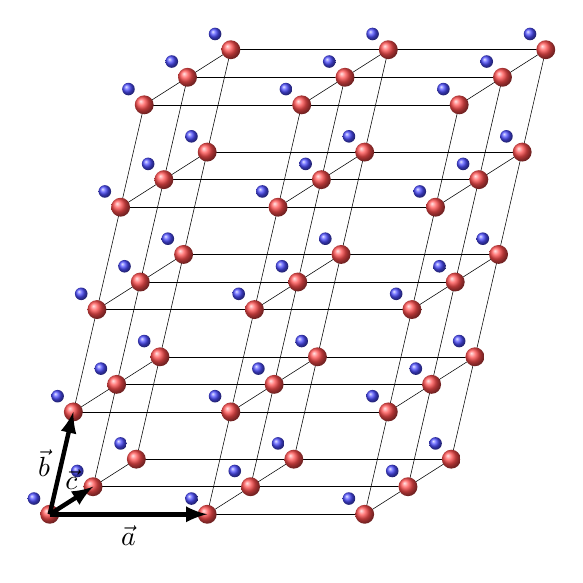
\begin{tikzpicture}[x  = {(1cm,0cm)},
  y  = {(0cm,1cm)},
  z  = {(0.35cm,0.35cm)},
  scale = 1]

  % angle
  % \filldraw[fill=red!35,draw=red!45,opacity=0.5]
  % (3,0.5) -- (1,0.5) arc (180:147:2) -- cycle;
  % \draw (1.75,0.6) node[above] {$\theta$};

  % grid
  % \draw[style=help lines,color=red!45][step=0.5cm] (-0.4,0.1) grid (6.4,2.4);
  % \draw[color=red!70, thick] (-0.4,0.5) -- (6.4,0.5);
  % \draw[->, >=latex, color=red!70, thick] (3,0.1) -- (3,3) node[left] {$\bf h$};

  \def\dax{2}
  \def\day{0.3}
  \def\daz{0.2}
  \def\dby{1.3}

  % grid
  \foreach \y in {0,1,...,4}
  \foreach \z in {0,1,...,2}
  \draw[style=help lines,color=black] (\dax*0+\day*\y+\daz*\z,\dby*\y,\z)
  -- (\dax*2+\day*\y+\daz*\z,\dby*\y,\z);

  \foreach \x in {0,1,...,2}
  \foreach \z in {0,1,...,2}
  \draw[style=help lines,color=black] (\dax*\x+\day*0+\daz*\z,\dby*0,\z)
  -- (\dax*\x+\day*4+\daz*\z,\dby*4,\z);

  \foreach \x in {0,1,...,2}
  \foreach \y in {0,1,...,4}
  \draw[style=help lines,color=black] (\dax*\x+\day*\y+\daz*0,\dby*\y,0)
  -- (\dax*\x+\day*\y+\daz*2,\dby*\y,2);

  % path to vector h
  % \draw[->, >=latex, ultra thick, color=green, style=dashed] (0,0,0) ->
  % +(\dax*3,0,0) -> +(\dax*3+\daz*1,0,1) -> (\dax*3+\day*2+\daz*1,\dby*2,1);

  % atoms
  \foreach \x in {0,1,...,2}
  \foreach \y in {0,1,...,4}
  \foreach \z in {0,1,...,2}
  {
  \shade[ball color=red!70] (\dax*\x+\day*\y+\daz*\z,\dby*\y,\z) circle (.12cm);
  \shade[ball color=blue!70] (\dax*\x+\day*\y+\daz*\z-0.2,\dby*\y+0.2,\z) circle (.08cm);
  }

  % unit cell
  \draw[->, >=latex, ultra thick] (0,0,0) -> node[left] {$\vec{b}$}
  (\day,\dby,0);
  \draw[->, >=latex, ultra thick, color=black]
  (0,0,0) -> node[below] {$\vec{a}$} (\dax,0,0);
  \draw[->, >=latex, ultra thick, color=black]
  (0,0,0) -> node[above] {$\vec{c}$} (\daz,0,1);

  % vector
  % \draw[->, >=latex, thick] (0,0,0) -> node[above] {$\vec h$}
  % (\dax*3+\day*2+\daz*1,\dby*2,1);
\end{tikzpicture}

%%% Local Variables:
%%% mode: latex
%%% TeX-master: "ChapterOne"
%%% End:

          \begin{lattice}{3}{6}{2}
            \begin{onlyenv}<2>
              \unitCell{0}
            \end{onlyenv}
          \end{lattice}
        \end{center}
      \end{overlayarea}

    \end{column}
  \end{columns}
\end{frame}

\begin{frame}[fragile]
  \frametitle{The Unit Cell}

  \begin{columns}
    \begin{column}{0.52\textwidth}
      \begin{overlayarea}{\textwidth}{\textheight}
      \begin{itemize}
      \item is the parallelepiped spanned by $\vec a$, $\vec b$,
        $\vec c$.
      \item is the smallest region that constitutes a repeating pattern.
      \item is characterized by the length and angles
        \begin{align*}
          a &= |\vec a|,\;  b = |\vec b|, \;c = |\vec c|\\
          \alpha &= \angle(\vec b,\vec c), \;
          \beta = \angle(\vec a,\vec c),\;
          \gamma = \angle(\vec b,\vec a).
        \end{align*}
      \end{itemize}

      \vspace{-0.3cm}
\begin{lstlisting}[style=input]
abc = [5.2, 5.2, 5.3]
abg = [90 99.25 90] * degree;
cs = crystalSymmetry('1',abc,abg)
\end{lstlisting}
      \vspace{-0.3cm}
\begin{lstlisting}[style=output]
ans = /+crystalSymmetry+/
  symmetry          : 1
  a, b, c           : 5.2, 5.2, 5.3
  alpha, beta, gamma: 90, 99.25, 90
\end{lstlisting}
    \end{overlayarea}
  \end{column}
  \begin{column}{0.45\textwidth}
    \begin{overlayarea}{\textwidth}{\textheight}

      \begin{center}
        \begin{lattice}{3}{6}{2}
          \unitCell{0}
        \end{lattice}
      \end{center}
    \end{overlayarea}
  \end{column}
  \end{columns}
\end{frame}


\begin{frame}[fragile]
  \frametitle{The Crystal Coordinate Systems}


  \begin{columns}
    \begin{column}{0.52\textwidth}
      \begin{overlayarea}{\textwidth}{\textheight}
        The vectors $\vec a$, $\vec b$, $\vec c$ constitute a right handed but
        non orthogonal coordinate system.

        \medskip

        \structure{Lattice points} are given by coordinates
        $u, v, w$:
        \begin{equation*}
          \structure{\cdot uvw\cdot} = \vec d = u \vec a + v \vec b + w \vec c.
        \end{equation*}
        \structure{Usage:} slip systems, dislocation systems
\begin{lstlisting}[style=input]
d = Miller(1,1,0,cs,'uvw')
\end{lstlisting}
        \begin{onlyenv}<1|handout:0> \vspace{-0.3cm}
\begin{lstlisting}[style=output]
d = /+Miller+/ (/+1+/)
  u  v  w
  1  1  0
\end{lstlisting}
          Smaller integers $u$, $v$, $w$ indicate higher density of lattice
          points on the line.
        \end{onlyenv}

        \medskip

        \begin{onlyenv}<2-> \structure{Lattice directions $[uvw]$:} all vectors
          parallel to $\vec d$

\begin{lstlisting}[style=input]
d == [2*d, -d]
\end{lstlisting}
        \end{onlyenv}
        \begin{onlyenv}<2|handout:0> \vspace{-0.3cm}
\begin{lstlisting}[style=output]
ans =

   1   0
\end{lstlisting}
          \end{onlyenv}
          \begin{onlyenv}<3->
            \vspace{-0.3cm}
\begin{lstlisting}[style=input]
[abs(d), norm(2*d)]
\end{lstlisting}
          \end{onlyenv}
          \begin{onlyenv}<3|handout:0> \vspace{-0.3cm}
\begin{lstlisting}[style=output]
ans =

    1.4142    2.8284
\end{lstlisting}
          \end{onlyenv}
          \begin{onlyenv}<4->
            \medskip
            \structure{Examples:} $[1 0 0]$,
          $[1 \overline 1 0] = [2 \overline 2 0] \ne [\overline 1 1 0]$
        \end{onlyenv}

      \end{overlayarea}
    \end{column}
    \begin{column}{0.45\textwidth}
      \begin{overlayarea}{\textwidth}{\textheight}
        \begin{onlyenv}<1->
          \begin{center}
            \begin{lattice}{3}{6}{2}
              \unitCell{0}
              \latticeVector{2}{3}{1}
            \end{lattice}
          \end{center}
        \end{onlyenv}
          \end{overlayarea}
        \end{column}
  \end{columns}
\end{frame}


\begin{frame}[fragile]
  \frametitle{The Reciprocal Coordinate System}

  \begin{columns}
    \begin{column}{0.52\textwidth}
      \begin{overlayarea}{\textwidth}{0.8\textheight}
        The reciprocal axes are orthogonal to $\vec a, \vec b, \vec c$,
        \begin{equation*}
          \vec a^{*} = \frac{\vec b \times \vec c}{V}, \;
          \vec b^{*} = \frac{\vec c \times \vec a}{V}, \;
          \vec c^{*} = \frac{\vec a \times \vec b}{V}
        \end{equation*}



        %\medskip

        %\structure{Properties:}

        \begin{itemize}
         \item $V = \vec a \cdot (\vec b \times \vec c)$ is the volume of the unit
          cell
        \item $\vec a \cdot \vec a^{*} = 1$, $\vec b \cdot \vec b^{*} = 1$, $\vec c \cdot \vec c^{*} = 1$
        \item units of $\vec a^{*}$, $\vec b^{*}$, $\vec c^{*}$ are reciprocal
          to $\vec a, \vec b, \vec c$
        \item for cubic lattices $\vec a || \vec a^{*}$, $\vec b || \vec b^{*}$, $\vec c || \vec c^{*}$,
        \end{itemize}

        \medskip

        Directions with respect to the $\vec a^{*}, \vec b^{*}, \vec c^{*}$ are given
        by integers coordinates $h$, $k$, $\ell$

  \begin{equation*}
    \vec n = h \vec a^{*} + k \vec b^{*} + \ell c^{*}
  \end{equation*}

% \begin{lstlisting}[style=input]
% n = Miller(1,1,0,cs,'hkl')
% \end{lstlisting}
%   \vspace{-0.3cm}
% \begin{lstlisting}[style=output]
% d = /+Miller+/
%  symmetry: 1
%   h 1
%   k 1
%   l 0
% \end{lstlisting}
\end{overlayarea}

\end{column}
\begin{column}{0.45\textwidth}
  \begin{overlayarea}{\textwidth}{\textheight}
    \begin{center}
      \begin{lattice}{3}{6}{2}
        \unitCell{0}

        \draw[->, >=latex, ultra thick] \latticePoint{0}{2}{0} -> +
        \reciprocalVector{3}{0}{0} node[right] {$\vec{a}^{*}$};
        \draw[->, >=latex, ultra thick] \latticePoint{0}{2}{0} ->
        + \reciprocalVector{0}{3}{0} node[above] {$\vec{b}^{*}$};
        \draw[->, >=latex, ultra thick] \latticePoint{0}{2}{0} ->
        + \reciprocalVector{0}{0}{3} node[right] {$\vec{c}^{*}$};

      \end{lattice}
    \end{center}
  \end{overlayarea}
\end{column}
\end{columns}
\end{frame}


\begin{frame}[fragile]
  \frametitle{The Reciprocal Coordinate System}

  \begin{columns}
    \begin{column}{0.52\textwidth}
      \begin{overlayarea}{\textwidth}{0.8\textheight}
\begin{lstlisting}[style=input]
n = Miller(1,1,0,cs,'hkl')
\end{lstlisting}
        \vspace{-0.3cm}
        \begin{onlyenv}<1|handout:0>
\begin{lstlisting}[style=output]
d = /+Miller+/ (/+1+/)
  h  k  l
  1  1  0
\end{lstlisting}
        \end{onlyenv}
        \begin{onlyenv}<2->
\begin{lstlisting}[style=input]
Miller({1,1,0},{0,1,1},cs,'hkl')
\end{lstlisting}
        \end{onlyenv}
        \vspace{-0.3cm}
        \begin{onlyenv}<2|handout:0>
\begin{lstlisting}[style=output]
ans = /+Miller+/ (/+1+/)
  h  k  l
  1  1  0
\end{lstlisting}
        \end{onlyenv}
        \begin{onlyenv}<3->
\begin{lstlisting}[style=input]
rec = [cs.aAxisRec,cs.bAxisRec,...
       cs.cAxisRec]
\end{lstlisting}
        \end{onlyenv}
        \begin{onlyenv}<4->
\begin{lstlisting}[style=input]
dot(rec,cs.aAxis)
\end{lstlisting}
        \end{onlyenv}
        \begin{onlyenv}<4|handout:0>
          \vspace{-0.3cm}
\begin{lstlisting}[style=output]
ans =

     1     0     0
\end{lstlisting}
        \end{onlyenv}
        \begin{onlyenv}<5->
\begin{lstlisting}[style=input]
cross(cs.aAxisRec,cs.bAxisRec)
\end{lstlisting}
        \end{onlyenv}
        \begin{onlyenv}<5|handout:0>
          \vspace{-0.3cm}
\begin{lstlisting}[style=output]
ans = /+Miller+/ (/+1+/)
  u  v  w
  0  0  1
\end{lstlisting}
        \end{onlyenv}

\end{overlayarea}

\end{column}
\begin{column}{0.45\textwidth}
  \begin{overlayarea}{\textwidth}{\textheight}
    \begin{center}
      \begin{lattice}{3}{6}{2}
        \unitCell{0}

        \draw[->, >=latex, ultra thick] \latticePoint{0}{2}{0} -> +
        \reciprocalVector{3}{0}{0} node[right] {$\vec{a}^{*}$};
        \draw[->, >=latex, ultra thick] \latticePoint{0}{2}{0} ->
        + \reciprocalVector{0}{3}{0} node[above] {$\vec{b}^{*}$};
        \draw[->, >=latex, ultra thick] \latticePoint{0}{2}{0} ->
        + \reciprocalVector{0}{0}{3} node[right] {$\vec{c}^{*}$};

      \end{lattice}
    \end{center}
  \end{overlayarea}
\end{column}
\end{columns}
\end{frame}

\begin{frame}
  \frametitle{Crystal Lattice Planes}

  \begin{columns}
    \begin{column}{0.52\textwidth}
      \begin{overlayarea}{\textwidth}{0.95\textheight}
        \begin{onlyenv}<1-> The plane $P$ normal to
          $\vec n = h \vec a^{*} + k \vec b^{*} + \ell c^{*}$ is
          \begin{equation*}
            P = \{\vec x \mid \vec x \cdot \vec n = d \} = \structure{(hk\ell)}.
          \end{equation*}
          It intersects the $\vec a$-axis in $\cdot u00 \cdot$ if
          \begin{equation*}
            d = u \vec a \cdot n
            = u \vec a \cdot (h \vec a^{*} + k \vec b^{*} + \ell c^{*}) = u h.
          \end{equation*}
        \end{onlyenv}%
        \begin{onlyenv}<2-> Hence, $(hk\ell)$ intersects $\vec a$, $\vec b$ and
          $\vec c$ in \structure{$\frac{d}{h},\, \frac{d}{k},\, \frac{d}{\ell}.$}
        \end{onlyenv}

        \bigskip

        \begin{onlyenv}<3-> Given axes intersections $m, n, p \in \mathbb
          N$. The corresponding normal vector is
          \begin{equation*}
            \vec n = \tfrac{d}{m} \vec a^{*} +  \tfrac{d}{n}  \vec b^{*} + \tfrac{d}{p}  \vec c^{*}
          \end{equation*}
          with $d = \mathrm{LCM}(m, n, p)$.
        \end{onlyenv}

        \medskip

        \begin{onlyenv}<4->
          $k = 0 \iff \frac{1}{0} = \infty \iff (hkl)$ is parallel to $\vec b$
        \end{onlyenv}


      \end{overlayarea}

    \end{column}
    \begin{column}{0.45\textwidth}
        \begin{overlayarea}{\textwidth}{\textheight}
          \begin{center}
            \begin{lattice}{3}{6}{2}

              \begin{onlyenv}<1-3>
                \draw[->, >=latex, ultra thick] \latticePoint{0}{0}{0} -> +
                \reciprocalVector{4}{2}{6} node[right, fill=white] {$\vec{n}=(213)$};

                \filldraw[fill=red!20,draw=red!40!black,opacity=0.5]
                \latticePoint{3}{0}{0} -- \latticePoint{0}{0}{2} --
                \latticePoint{0}{6}{0} -- cycle;

                \draw[-, ultra thick] \latticePoint{0}{0}{0} -> +
                \reciprocalVector{2}{1}{3};
              \end{onlyenv}

              \begin{onlyenv}<4|handout:0>

                \draw[->, >=latex, ultra thick] \latticePoint{0}{2}{0} -> +
                \reciprocalVector{2}{0}{0} node[right, fill=white]
                {$\vec{n}=(100)$};

                \filldraw[fill=red!20,draw=red!40!black,opacity=0.5]
                \latticePoint{1}{0}{0} -- \latticePoint{1}{0}{2} --
                \latticePoint{1}{6}{2} --
                \latticePoint{1}{6}{0} -- cycle;

              \end{onlyenv}

              \begin{onlyenv}<5|handout:0>

                \draw[->, >=latex, ultra thick] \latticePoint{0}{0}{0} -> +
                \reciprocalVector{0}{2}{0} node[above, fill=white]
                {$\vec{n}=(010)$};

                \filldraw[fill=red!20,draw=red!40!black,opacity=0.5]
                \latticePoint{0}{1}{0} -- \latticePoint{3}{1}{0} --
                \latticePoint{3}{1}{2} --
                \latticePoint{0}{1}{2} -- cycle;

              \end{onlyenv}



              % \filldraw[fill=red!20,draw=red!40!black,opacity=0.5] (\dax*3,0,0) --
              % (\daz*2,0,2) -- (\day*6,\dby*6,0) -- cycle;

            \end{lattice}
          \end{center}
        \end{overlayarea}
      \end{column}
    \end{columns}
\end{frame}



\begin{frame}
  \frametitle{Miller Indices}
%  \left<hk\ell\right>

    \begin{columns}
    \begin{column}{0.52\textwidth}
      \begin{overlayarea}{\textwidth}{0.95\textheight}
          The lattice plane $(123)$ perpendicular to
  $\vec n = \vec a^{*} + 2 \vec b^{*} + 3 \vec c^{*}$ which intersects the
  direct lattice axes $\vec{a}$, $\vec{b}$ and $\vec{c}$ at $1$, $\tfrac12$ and
  $\tfrac13$.

  \begin{itemize}
  \item The coordinates $h$, $k$, $\ell$ are the \structure{Miller indices} of the plane $P$.
  \item planes $(hk\ell)$ parallel to $\vec a$ have interception point
    $\frac{1}{\infty}$ and hence $h=0$
  \item planes $(h 0 0)$ perpendicular to $\vec a^{*}$ have interception
    points $(\frac{d}{h},\frac{1}{\infty},\frac{1}{\infty})$
  \end{itemize}

      \end{overlayarea}
    \end{column}
    \begin{column}{0.45\textwidth}
        \begin{overlayarea}{\textwidth}{\textheight}
          \begin{center}
            \begin{lattice}{3}{6}{2}

              % \filldraw[fill=red!20,draw=red!40!black,opacity=0.5] (\dax*3,0,0) --
              % (\daz*2,0,2) -- (\day*6,\dby*6,0) -- cycle;

            \end{lattice}
          \end{center}
        \end{overlayarea}
    \end{column}
  \end{columns}

\end{frame}


\begin{frame}[fragile]
  \frametitle{The Zone Equation}

  \begin{columns}
    \begin{column}{0.52\textwidth}
      \begin{overlayarea}{\textwidth}{0.9\textheight}
        \begin{onlyenv}<1-> A direction $[uvw]$ is parallel to a plane
          $(hk\ell)$ if
          \begin{equation*}
            h u + k v + \ell w = 0.
          \end{equation*}
        \end{onlyenv}

        \medskip

        \begin{onlyenv}<3-> The plane $(hkl)$ spanned by the directions
          $[u_{1}v_{1}w_{1}]$ and $[u_{2}v_{2}w_{2}]$:
          \begin{equation*}
            (hkl) = [u_{1}v_{1}w_{1}] \times [u_{2}v_{2}w_{2}]
          \end{equation*}
        \end{onlyenv}
        \medskip

        \begin{onlyenv}<4-> The common direction $[uvw]$ of two planes
          $(h_{1}k_{1}\ell_{1})$ and $(h_{2}k_{2}\ell_{2})$
          \begin{equation*}
            [uvw] = (h_{1}k_{1}\ell_{1}) \times (h_{2}k_{2}\ell_{2})
          \end{equation*}
        \end{onlyenv}

      \end{overlayarea}

    \end{column}
    \begin{column}{0.45\textwidth}
      \begin{overlayarea}{\textwidth}{0.95\textheight}
        \begin{onlyenv}<1->
\begin{lstlisting}[style=input]
d1 = Miller(1,-1,2,cs,'uvw')
n1 = Miller(1,1,0,cs,'hkl')
dot(d1,n1)
\end{lstlisting}
        \end{onlyenv}
        \vspace{-0.3cm}
        \begin{onlyenv}<1|handout:0>
\begin{lstlisting}[style=output]
ans =

   7.7716e-16
\end{lstlisting}
        \end{onlyenv}
        \begin{onlyenv}<2->
\begin{lstlisting}[style=input]
angle(n1,d2) ./ degree
\end{lstlisting}
        \end{onlyenv}
        \begin{onlyenv}<2|handout:0>
\begin{lstlisting}[style=output]
ans =

   90.0000
\end{lstlisting}
        \end{onlyenv}

        \begin{onlyenv}<3->
\begin{lstlisting}[style=input]
d2 = Miller(1,0,0,cs,'uvw')
cross(d1,d2)
\end{lstlisting}
        \end{onlyenv}
        \begin{onlyenv}<3|handout:0>
          \vspace{-0.3cm}
\begin{lstlisting}[style=output]
ans = /+Miller+/ (/+1+/)
  h  k  l
  0  2  1
\end{lstlisting}
        \end{onlyenv}
        \begin{onlyenv}<4->
\begin{lstlisting}[style=input]
n2 = Miller(1,0,0,cs,'hkl')
cross(n1,n2)
\end{lstlisting}
          \vspace{-0.3cm}
\begin{lstlisting}[style=output]
ans = /+Miller+/ (/+1+/)
 u  v  w
 0  0 -1
\end{lstlisting}
        \end{onlyenv}
      \end{overlayarea}



\end{column}
\end{columns}
\end{frame}


\begin{frame}[fragile]
  \frametitle{Morphology}

  Crystals are formed by crystallization from a solution or a melt.

  the two steps of crystallization:    nucleation and growth

  \pause

  \begin{columns}
    \begin{column}{0.6\textwidth}

      \begin{itemize}
      \item<+-> the grow rate is an anisotropic property
      \item<+-> lattice planes with high grow rate get smaller
      \item<+-> lattice planes with low grow rate become larger
      \item<+-> lattice planes $(hk\ell)$ with small Miller indices usually have high
        density and grow slowly
      \item<+-> the shape of a crystal is formed by its low index lattice planes
      \item<+-> law of constant dihedral angles
      \end{itemize}

      \begin{lstlisting}[style=input]
cs = crystalSymmetry.load('quartz.cif')
cS = crystalShape.quartz;
plot(cS,'colored')
      \end{lstlisting}

      
    \end{column}
    \begin{column}{0.3\textwidth}

      \begin{center}
        \begin{onlyenv}<1-6>
          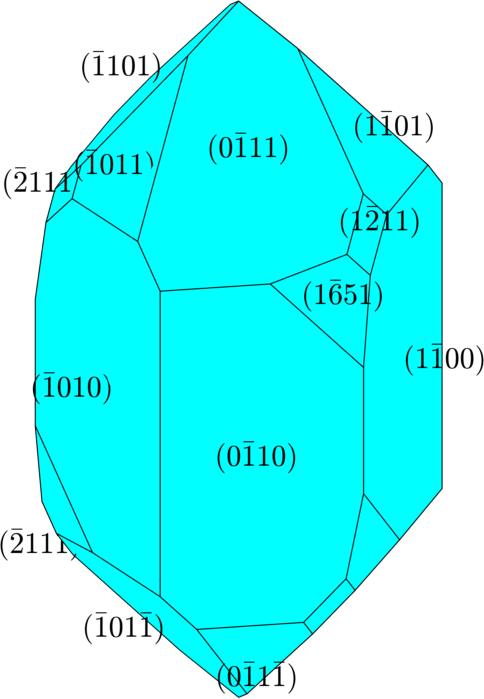
\includegraphics[width=\textwidth]{pic/quartzMiller}
        \end{onlyenv}
        \begin{onlyenv}<7-|handout:0>
          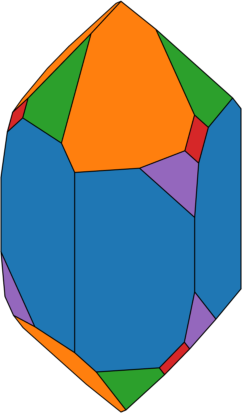
\includegraphics[width=0.85\textwidth]{pic/quartzMillerColor}
        \end{onlyenv}
      \end{center}

    \end{column}
  \end{columns}

\end{frame}


% \begin{frame}[fragile]
%   \frametitle{Crystal Shapes in MTEX}

%   \begin{overlayarea}{\textwidth}{0.8\textheight}
% \begin{lstlisting}[style=input]
% cs = crystalSymmetry.load('Mg-Magnesium.cif')
% \end{lstlisting}

%     \begin{only}<1>
% \begin{lstlisting}[style=output]
% cs = crystalSymmetry (show methods, plot)

%   mineral        : Mg
%   symmetry       : 6/mmm
%   elements       : 24
%   a, b, c        : 3.2, 3.2, 26
%   reference frame: X||a*, Y||b, Z||c*
% \end{lstlisting}
%     \end{only}

% \begin{lstlisting}[style=input]
% cS = crystalShape.hex(cs)
% \end{lstlisting}
% \begin{lstlisting}[style=output]
% cS = crystalShape (show methods, plot)
%  mineral: Mg (6/mmm, X||a*, Y||b, Z||c*)
%  vertices: 12
%  faces: 8
% \end{lstlisting}

%   \end{overlayarea}
% \end{frame}


\begin{frame}
  \frametitle{The Crystal Planes of Quartz  in a Stereographic Projection}

  \begin{columns}
    \begin{column}{0.5\textwidth}
      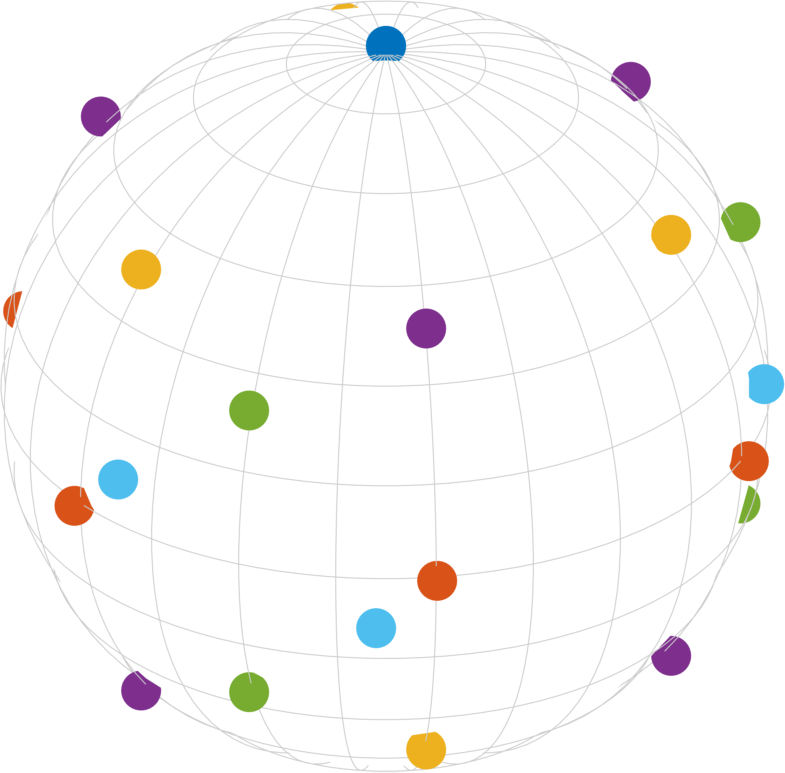
\includegraphics[width=\textwidth]{pic/proj3d.png}
    \end{column}
    \begin{column}{0.3\textwidth}
      \begin{itemize}
      \item[\textcolor{Matlab1}{c}] \structure{c-axis:} \\
        $(0001)$, $(000\overline{1})$
      \item[\textcolor{Matlab6}{m}] \structure{hexagonal prism:} \\
        $(10\overline{1}0)$, $(01\overline{1}0)$,$(1\overline{1}00)$\\
        $(\overline{1}010)$, $(0\overline{1}10)$,$(\overline{1}100)$\\
      \item[\textcolor{Matlab2}{r}] \structure{positive rhomboedron:}
        $(10\overline{1}1$, $(\overline{1}101)$, $(0\overline{1}11)$
      \item[\textcolor{Matlab3}{z}] \structure{negative rhombodron:}
        $(1\overline{1}01)$,$(01\overline{1}1)$,$(\overline{1}011)$
      \item[\textcolor{Matlab4}{s}] \structure{trigonal bipyramid:}
        $(11\overline{2}1)$, $(1\overline{2}11)$, $(\overline{2}111)$
      \item[\textcolor{Matlab5}{x}] \structure{positive trapezohedron:}
        $(51\overline{6}1)$, $(\overline{6}511)$, $(1\overline{6}51)$
      \end{itemize}
    \end{column}
  \end{columns}
\end{frame}



% \begin{frame}
%   \frametitle{Crystals Structure}

%   \begin{center}
%     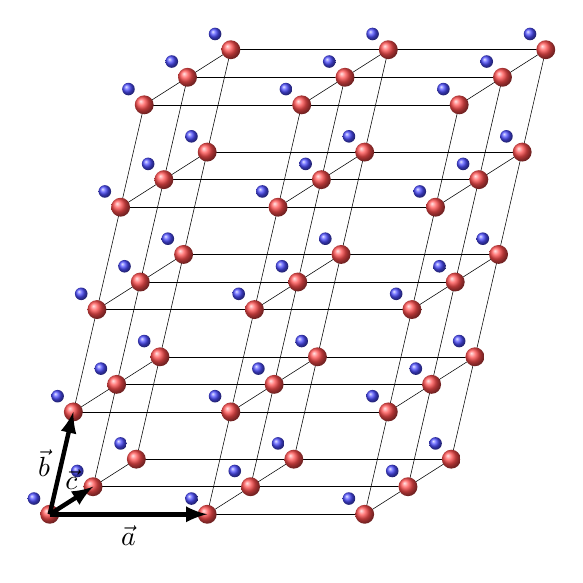
\begin{tikzpicture}[x  = {(1cm,0cm)},
  y  = {(0cm,1cm)},
  z  = {(0.35cm,0.35cm)},
  scale = 1]

  % angle
  % \filldraw[fill=red!35,draw=red!45,opacity=0.5]
  % (3,0.5) -- (1,0.5) arc (180:147:2) -- cycle;
  % \draw (1.75,0.6) node[above] {$\theta$};

  % grid
  % \draw[style=help lines,color=red!45][step=0.5cm] (-0.4,0.1) grid (6.4,2.4);
  % \draw[color=red!70, thick] (-0.4,0.5) -- (6.4,0.5);
  % \draw[->, >=latex, color=red!70, thick] (3,0.1) -- (3,3) node[left] {$\bf h$};

  \def\dax{2}
  \def\day{0.3}
  \def\daz{0.2}
  \def\dby{1.3}

  % grid
  \foreach \y in {0,1,...,4}
  \foreach \z in {0,1,...,2}
  \draw[style=help lines,color=black] (\dax*0+\day*\y+\daz*\z,\dby*\y,\z)
  -- (\dax*2+\day*\y+\daz*\z,\dby*\y,\z);

  \foreach \x in {0,1,...,2}
  \foreach \z in {0,1,...,2}
  \draw[style=help lines,color=black] (\dax*\x+\day*0+\daz*\z,\dby*0,\z)
  -- (\dax*\x+\day*4+\daz*\z,\dby*4,\z);

  \foreach \x in {0,1,...,2}
  \foreach \y in {0,1,...,4}
  \draw[style=help lines,color=black] (\dax*\x+\day*\y+\daz*0,\dby*\y,0)
  -- (\dax*\x+\day*\y+\daz*2,\dby*\y,2);

  % path to vector h
  % \draw[->, >=latex, ultra thick, color=green, style=dashed] (0,0,0) ->
  % +(\dax*3,0,0) -> +(\dax*3+\daz*1,0,1) -> (\dax*3+\day*2+\daz*1,\dby*2,1);

  % atoms
  \foreach \x in {0,1,...,2}
  \foreach \y in {0,1,...,4}
  \foreach \z in {0,1,...,2}
  {
  \shade[ball color=red!70] (\dax*\x+\day*\y+\daz*\z,\dby*\y,\z) circle (.12cm);
  \shade[ball color=blue!70] (\dax*\x+\day*\y+\daz*\z-0.2,\dby*\y+0.2,\z) circle (.08cm);
  }

  % unit cell
  \draw[->, >=latex, ultra thick] (0,0,0) -> node[left] {$\vec{b}$}
  (\day,\dby,0);
  \draw[->, >=latex, ultra thick, color=black]
  (0,0,0) -> node[below] {$\vec{a}$} (\dax,0,0);
  \draw[->, >=latex, ultra thick, color=black]
  (0,0,0) -> node[above] {$\vec{c}$} (\daz,0,1);

  % vector
  % \draw[->, >=latex, thick] (0,0,0) -> node[above] {$\vec h$}
  % (\dax*3+\day*2+\daz*1,\dby*2,1);
\end{tikzpicture}

%%% Local Variables:
%%% mode: latex
%%% TeX-master: "ChapterOne"
%%% End:

%   \end{center}

%   \begin{center}
%     crystals structure = basis + lattice
%   \end{center}

% \end{frame}


% \begin{frame}
%   \frametitle{Crystals Structure}

%   \begin{center}
%     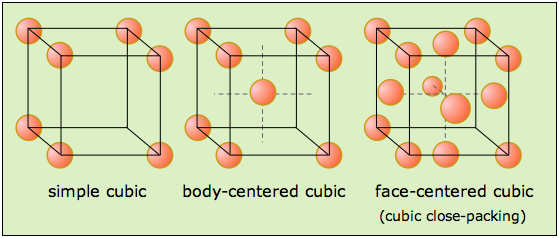
\includegraphics[width=\textwidth]{pic/fccbcc.png}
%   \end{center}

%   \begin{center}
%     crystals structure = basis + lattice
%   \end{center}

% \end{frame}


% \def\radius{6}
% \def\Alpha{20}
% \def\Beta{20}
% \def\Gamma{20}

% \tdplotsetmaincoords{70}{150}

% \tikzset{% Some styles. More could be done.
%     axis/.style={very thick, fill=white, -*, shorten >=-3pt},
%     axis'/.style={thick, -},
%     axis''/.style={thick, -},
%     Axis/.style={very thick, fill=black, -*, shorten >=-3pt},
%     behind lines/.style={loosely dashed}
% }

% \begin{tikzpicture}[tdplot_main_coords]

% \begin{scope}[scale=\radius, every path/.style={tdplot_rotated_coords}]

% % Back half of the white circle.
% \tdplotsetrotatedcoords{\Alpha}{0}{0}
% \draw  [fill=white]
%     plot    [domain=90:270, samples=100] (cos \x, sin \x) -- cycle;

% % The light gray circle
% \tdplotsetrotatedcoords{\Alpha}{\Beta}{\Gamma}
% \draw  [fill=gray!20]
%     plot    [domain=0:360, samples=100] (cos \x, sin \x);

% % The dashed edge of the back half of the white circle
% \begin{scope}
% \tdplotsetrotatedcoords{\Alpha}{\Beta}{\Gamma}
% \path  [clip]
%     plot    [domain=0:360, samples=100] (cos \x, sin \x);

% \tdplotsetrotatedcoords{\Alpha}{0}{0}
% \draw  [behind lines]
%     plot    [domain=90:270, samples=100] (cos \x, sin \x);
% \end{scope}

% % The upper (unfilled) semi circles
% \tdplotsetrotatedcoords{\Alpha}{90}{0}
% \draw [domain=90:270, samples=100] plot (cos \x, sin \x);
% \tdplotsetrotatedcoords{\Alpha+90}{90}{0}
% \draw [domain=90+\Beta:270+\Beta, samples=100] plot (cos \x, sin \x);


% % The dark gray sector
% \tdplotsetrotatedcoords{\Alpha-90}{-90}{90}
% \draw [fill=gray, thick, domain=0:\Beta]
%     (0,0) -- plot (cos \x, sin \x) -- cycle;

% % The X axis
% \tdplotsetrotatedcoords{\Alpha}{\Beta}{\Gamma}
% \draw[Axis] (0,0,0) -- (1,0,0) node [below left] {$X$};

% % The x'' axis
% \tdplotsetrotatedcoords{\Alpha}{\Beta}{0}
% \draw[axis'] (0,0,0) -- (1,0,0) node [below left] {$x''$};

% % The front half of the white circle
% \tdplotsetrotatedcoords{\Alpha}{0}{0}
% \draw  [fill=white]
%     plot [domain=-90:0, samples=100] (cos \x, sin \x)
%     .. controls (0.125*cos 22.5, 0.125*sin 22.5) ..
%     (cos 45, sin 45) -- plot    [domain=45:90, samples=100] (cos \x, sin \x)
%     -- cycle;

% % The dashed lines in the front half of the white circle
% \begin{scope}
% \tdplotsetrotatedcoords{\Alpha}{0}{0}
% \path  [clip]
%     plot [domain=-90:0, samples=100] (cos \x, sin \x)
%     .. controls (0.125*cos 22.5, 0.125*sin 22.5) ..
%     (cos 45, sin 45) -- plot    [domain=45:90, samples=100] (cos \x, sin \x)
%     -- cycle;

% \tdplotsetrotatedcoords{\Alpha-90}{-90}{90}
% \draw [behind lines] (0,0) -- (cos \Beta, sin \Beta);

% \tdplotsetrotatedcoords{\Alpha}{\Beta}{\Gamma}
% \draw [behind lines] (0,0,0) -- (1,0,0);

% \end{scope}


% % Axes x, y, z
% \tdplotsetrotatedcoords{0}{0}{0}
% \draw[axis] (0,0,0) -- (1,0,0) node [below left]  {$x$};
% \draw[axis] (0,0,0) -- (0,1,0) node [below right] {$y$};
% \draw[axis] (0,0,0) -- (0,0,1) node [above=0.1cm] {$z=z'$};

% % Axis x'
% \tdplotsetrotatedcoords{\Alpha}{0}{0}
% \draw[axis] (0,0,0) -- (1,0,0) node [below left] {$x'$};

% % Axes Y
% \tdplotsetrotatedcoords{\Alpha}{\Beta}{\Gamma}
% \draw[Axis] (0,0,0) -- (0,1,0) node [right] {$Y$};
% % Axes z' and Z
% \draw[Axis] (0,0,0) -- (0,0,1) node [left=0.1cm] {$z''=Z$};

% % Axes y' and y''
% \tdplotsetrotatedcoords{\Alpha}{\Beta}{0}
% \draw[axis'] (0,0,0) -- (0,1,0) node [below right] {$y'=y''$};

% % Arrows
% \tdplotsetrotatedcoords{0}{0}{0}
% \tdplotdrawarc[-latex]{(0,0,0)}{0.8}{0}{\Alpha}{below left=0cm}{$\alpha$}
% \tdplotsetrotatedcoords{\Alpha+90}{90}{0}
% \tdplotdrawarc[-latex]{(0,0,0)}{0.8}{-90}{-90+\Beta}{left}{$\beta$}
% \tdplotsetrotatedcoords{\Alpha}{\Beta}{\Gamma}
% \tdplotdrawarc[-latex]{(0,0,0)}{0.8}{-\Gamma}{0}{below}{$\gamma$}

% \tdplotsetrotatedcoords{0}{0}{0}
% \tdplotdrawarc[-latex]{(0,0,0)}{0.8}{90}{90+\Alpha}{above left=0cm}{$\alpha$}
% \tdplotsetrotatedcoords{\Alpha+90}{90}{0}
% \tdplotdrawarc[-latex]{(0,0,0)}{0.8}{-180}{-180+\Beta}{above}{$\beta$}
% \tdplotsetrotatedcoords{\Alpha}{\Beta}{\Gamma}
% \tdplotdrawarc[-latex]{(0,0,0)}{0.8}{90-\Gamma}{90}{left}{$\gamma$}

% \end{scope}

% \end{tikzpicture}


\begin{frame}
  \frametitle{Active vs. Passive Rotations}

  \begin{columns}[T,onlytextwidth]
    \begin{column}{0.6\textwidth}
      \begin{block}{Active Rotations}
        An active rotation is a mapping of the Euclidean space onto itself
        that keeps at least one point and all distances invariant and
        preserves orientation.
      \end{block}

  \begin{block}{Passive Rotations}
    A passive rotation is a coordinate transform from one right handed, orthonormal
    coordinate system into another one.
  \end{block}

  \begin{block}{Improper Rotations}
    An improper rotation is a rotation that switches between left handed and
    right handed coordinate systems.
  \end{block}

\end{column}
\begin{column}{0.35\textwidth}

  the matrix $\mat M =
  \begin{pmatrix}
    | & | & | \\
    \vec v_{1} & \vec v_{2} & \vec v_{3}\\
    | & | & |
  \end{pmatrix}$ rotates \\
  $\vec e_{1} \mapsto \vec v_{1}$, $\vec e_{2} \mapsto \vec v_{2}$,
  $\vec e_{3} \mapsto \vec v_{3}$ \\


  \vspace{0.5cm}

  $\mat M$ transforms coordinates from
  the reference frame $(\vec v_{1}, \vec v_{2}, \vec v_{3})$ into the
  reference frame $(\vec e_{1}, \vec e_{2}, \vec e_{3})$

  \vspace{0.5cm}

  $\tilde{\mat M} = -\mat M$ additionally mirrors all vectors at the origin

  \vspace{1cm}

\end{column}
\end{columns}

\end{frame}



% \begin{frame}
%   \frametitle{Rotation Matrices}

%   A matrix $\mat R \in \mathbb R^{3 \times 3}$ is called
%   \begin{itemize}
%   \item \structure{orthogonal} if $ \mat R^{-1} = \mat R^{T}$
%   \item \structure{(proper) rotation} if it is orthogonal and $\det \mat R
%     = 1$
%   \item \structure{improper rotation} if it is orthogonal and $\det \mat R
%     = -1$
%   \end{itemize}

%   \pause
%   \bigskip

%   Let $\vec X_{1}, \vec Y_{1}, \vec Z_{1}$ be right handed orthonormal
%   coordinate system. Then
%   \begin{itemize}
%   \item $\mat R \vec X_{1}, \mat R \vec Y_{1}, \mat R \vec Z_{1}$ is
%     again an orthonormal coordinate system
%   \item if $\mat R$ is proper, then $\mat R \vec X_{1}, \mat R \vec
%     Y_{1}, \mat R \vec Z_{1}$ is again right handed
%   \item if $\mat R$ is improper, then $\mat R \vec X_{1}, \mat R \vec
%     Y_{1}, \mat R \vec Z_{1}$ is left handed
%   \end{itemize}

%   \pause
%   \bigskip

%   \structure{Active rotation:} Given two orthonormal bases
%   $(\vec X_{1}, \vec Y_{1}, \vec Z_{1})$ and
%   $(\vec X_{2}, \vec Y_{2}, \vec Z_{2})$ the \emph{active rotation}
%   $\mat R$ such that $\vec X_{2} = \mat{R} \vec X_{1}$, $\vec Y_{2} =
%   \mat{R} \vec Y_{1}$ and $\vec Z_{2} = \mat{R} \vec Z_{1}$ is given by

%   \begin{equation*}
%     \mat R =
%     (\vec X_{2}, \vec Y_{2}, \vec Z_{2}) \cdot
%     (\vec X_{1}, \vec Y_{1}, \vec Z_{1})^{t}
%     =
%     \begin{pmatrix}
%       | & | & | \\
%       \vec X_{2} & \vec Y_{2} & \vec Z_{2}\\
%       | & | & |
%     \end{pmatrix}
%     \begin{pmatrix}
%       \text{---}\; X_{1}^{t}\;\text{---}\\
%       \text{---}\;\vec Y_{1}^{t}\;\text{---}\\
%       \text{---}\;\vec Z_{1}^{t}\;\text{---}
%     \end{pmatrix}
%   \end{equation*}
% \end{frame}


\begin{frame}[fragile]
  \frametitle{Defining Active Rotations}

  \begin{columns}[T,onlytextwidth]
    \begin{column}{0.49\textwidth}
      \begin{overlayarea}{\textwidth}{0.85\textheight}

    by axis angle \vspace{-0.2cm}
\begin{lstlisting}[style=input]
v = vector3d(1,0,0)
w = 90*degree
r = rotation.byAxisAngle(v,w)
\end{lstlisting}
    \begin{onlyenv}<1> \vspace{-0.4cm}
      \begin{lstlisting}[style=output]
r = /+rotation+/

  Bunge Euler angles in degree
  phi1  Phi  phi2  Inv.
     0   90     0    0
\end{lstlisting}
    \end{onlyenv}

    \begin{onlyenv}<2->
      by Euler angles\vspace{-0.2cm}
      \begin{lstlisting}[style=input]
r = rotation.byEuler(0,0,pi/2)
\end{lstlisting}
    \end{onlyenv}
    \begin{onlyenv}<2>\vspace{-0.4cm}
      \begin{lstlisting}[style=output]
r = /+rotation+/

  Bunge Euler angles in degree
  phi1  Phi  phi2  Inv.
    90    0     0    0
      \end{lstlisting}
    \end{onlyenv}

    \begin{onlyenv}<3->
      by a rotation matrix\vspace{-0.2cm}
\begin{lstlisting}[style=input]
M = [1 0 0; 0 0 -1; 0 1 0]
r = rotation.byMatrix(M)
\end{lstlisting}
    \end{onlyenv}
    \begin{onlyenv}<3> \vspace{-0.4cm}
      \begin{lstlisting}[style=output]
r = /+rotation+/

  Bunge Euler angles in degree
  phi1  Phi  phi2  Inv.
     0   90     0    0
      \end{lstlisting}
    \end{onlyenv}

    \begin{onlyenv}<4->
      by pairs of vectors\vspace{-0.2cm}
      \begin{lstlisting}[style=input]
u1 = vector3d.Z; v1 = u1
u2 = vector3d.X; v2 = vector3d.Y
r  = rotation.map(u1,v1,u2,v2)
\end{lstlisting}
    \end{onlyenv}

    \begin{onlyenv}<5->
      \begin{lstlisting}[style=input]
r  = rotation.fit(u, v)
\end{lstlisting}
    \end{onlyenv}

  \end{overlayarea}
    \end{column}

    \begin{column}{0.485\textwidth}
  \begin{overlayarea}{\textwidth}{0.85\textheight}

    \begin{onlyenv}<6-> import rotations\vspace{-0.2cm}
      \begin{lstlisting}[style=input]
r = rotation.load('file.txt',...
  'ColumnNames',...
  {'phi1','Phi','phi2'})
      \end{lstlisting}
    \end{onlyenv}
    \begin{onlyenv}<6>\vspace{-0.4cm}
      \begin{lstlisting}[style=output]
r = /+rotation+/
  size: 1 x 100
      \end{lstlisting}
    \end{onlyenv}

    \begin{onlyenv}<7-> random rotations\vspace{-0.2cm}
      \begin{lstlisting}[style=input]
r = rotation.rand(100)
      \end{lstlisting}
    \end{onlyenv}
    \begin{onlyenv}<7>\vspace{-0.4cm}
      \begin{lstlisting}[style=output]
r = /+rotation+/
  size: 1 x 100
      \end{lstlisting}
    \end{onlyenv}


    \begin{onlyenv}<8-> identity and inversion \vspace{-0.2cm}
      \begin{lstlisting}[style=input]
r = rotation.id
r = rotation.inversion
      \end{lstlisting}
    \end{onlyenv}
    \begin{onlyenv}<8>\vspace{-0.4cm}
      \begin{lstlisting}[style=output]
r = /+rotation+/

  Bunge Euler angles in degree
  phi1  Phi phi2 Inv.
     0    0    0    0
     0    0    0    1
      \end{lstlisting}
    \end{onlyenv}

    \begin{onlyenv}<9-> a reflextion\vspace{-0.2cm}
      \begin{lstlisting}[style=input]
r = reflection(vector3d.X)
      \end{lstlisting}
    \end{onlyenv}
    \begin{onlyenv}<9>\vspace{-0.4cm}
      \begin{lstlisting}[style=output]
r = /+rotation+/

  Bunge Euler angles in degree
  phi1  Phi phi2 Inv.
     0  180    0    1
      \end{lstlisting}
    \end{onlyenv}

  \end{overlayarea}
\end{column}

  \end{columns}

\end{frame}


\begin{frame}[fragile]
  \frametitle{Euler Angles}

  \begin{Definition}[Euler angles]
    Let $\varphi_{1},\varphi_{2} \in [0,2\pi]$ and $\Phi \in [0,\pi]$. Then
    $\varphi_{1},\Phi,\varphi_{2}$ are called the \structure{Euler angles} of
    the rotation
    \begin{equation*}
      \mat R(\varphi_{1},\Phi,\varphi_{2})
      = \mat R_{\vec Z,\varphi_{1}} \mat R_{\vec X,\Phi}  \mat R_{\vec Z,\varphi_{2}}.
    \end{equation*}
  \end{Definition}

\begin{lstlisting}[style=input]
rot = rotation.byEuler(10*degree,20*degree,30*degree)
\end{lstlisting}



  \begin{itemize}
  \item<+-> For every rotation $\mat R$ there are Euler angles
    $\varphi_{1},\Phi,\varphi_{2}$ such that
    $\mat R = \mat R(\varphi_{1},\Phi,\varphi_{2})$.
  \item For specific rotations $\rot R$ the Euler angles are not unique, e.g.
    \begin{equation*}
      \mat R_{\vec z,\omega} = \mat R(\varphi_{1},0,\omega-\varphi_{1})
    \end{equation*}
  \item Euler angles are the most common way to specify and visualize rotations in texture
    analysis.
  \item The ambiguity makes visualization with respect to Euler angles hard to interpret.
  \end{itemize}

\end{frame}


\begin{frame}[fragile,fragile]
  \frametitle{Operations with Rotations}

  \vspace{-0.5cm}

  \begin{columns}[t]
    \begin{column}{0.47\textwidth}

      vector rotation \vspace{-0.2cm}
\begin{lstlisting}[style=input]
v = rot .* u
\end{lstlisting}

      concatenation \vspace{-0.2cm}
\begin{lstlisting}[style=input]
rot = rot1 .* rot2
v = rot .* u
v = rot1 * (rot2 * u)
\end{lstlisting}

     inverse of a rotation / misrotation \vspace{-0.2cm}
\begin{lstlisting}[style=input]
inv(rot1)
inv(rot1) .* rot2
\end{lstlisting}

basic statistics \vspace{-0.2cm}
\begin{lstlisting}[style=input]
mean(rot)
mean(rot,'weights',w)
std(rot)

unique(rot)
\end{lstlisting}



    \end{column}

  \begin{column}{0.47\textwidth}

convert to Euler angles \vspace{-0.2cm}
\begin{lstlisting}[style=input]
[phi1,Phi,phi2] = Euler(rot)
\end{lstlisting}

axis / angle \vspace{-0.2cm}
\begin{lstlisting}[style=input]
rot.axis, rot.angle
angle(rot1,rot2)
\end{lstlisting}

convert to matrix \vspace{-0.2cm}
\begin{lstlisting}[style=input]
rot.matrix
\end{lstlisting}

convert to quaternion \vspace{-0.2cm}
\begin{lstlisting}[style=input]
[a,b,c,d] = double(rot)
quaternion(rot)
\end{lstlisting}

convert to rotation vectors \vspace{-0.2cm}
\begin{lstlisting}[style=input]
rot.Rodrigues
rot.homochoric
rot.cubochoric
\end{lstlisting}

  \end{column}

  \end{columns}
\end{frame}



% \begin{frame}
%   \frametitle{Rodrigues Frank Space}

%   \begin{Definition}[Rodrigues Frank Vector]
%     \begin{equation*}
%       \vec r = \tan \frac{\omega}2 \vec v
%     \end{equation*}
%   \end{Definition}


%   Properties:
%   \begin{itemize}
%   \item rotations fill entire $\R^{3}$
%   \item identical rotation is mapped to $(0,0,0)$
%   \item rotations with rotational angle $\pi$ are mapped to infinity
%   \item rotations $\omega \mapsto \mat R_{\vec v,\omega}$ about a fixed axis
%     become straight lines
%   \item rotations with the same distance to two given rotations $\mat R_{1}$,
%     $\mat R_{2}$ become a plane
%   \end{itemize}

% \end{frame}

% \begin{frame}
%   \frametitle{Axis Angle Space}


%   \begin{Definition}[Rotation Vector]
%     \begin{equation*}
%       \vec r = \omega \vec v
%     \end{equation*}
%   \end{Definition}


%     Properties:
%   \begin{itemize}
%   \item rotations fill the ball $\mathbb B^{3} = \{\vec x \in \R^{3}\mid
%     \norm{\vec x} = \pi\} $
%   \item identical rotation is mapped to $(0,0,0)$
%   \item rotations with rotational angle $\pi$ are mapped to the boundary
%   \item antipodal boundary points describe the same rotation, i.e., $\vec r =
%     -\vec r$ for $\norm{\vec v}=\pi$
%   \item Euclidean distance to the origin $(0,0,0)$ is rotational angle
%   \item Euclidean distance between two arbitrary rotations is slightly
%     different then their rotational angle
%   \end{itemize}

% \end{frame}

\begin{frame}[fragile]
  \frametitle{Visualizing Rotations}


  \begin{columns}[T,onlytextwidth]
    \begin{column}{0.425\textwidth}

      Euler angle space
      \vspace{-0.2cm}
      \begin{lstlisting}[style=input]
rot = rotation.rand
plot(rot)
\end{lstlisting}

\pause
\medskip

axis angle space \vspace{-0.2cm}
      \begin{lstlisting}[style=input]
plot(rot,'axisAngle')
\end{lstlisting}

%       \begin{lstlisting}[style=input]
% plot(rot,'Rodrigues')
% \end{lstlisting}

\pause
\medskip

Euler angle $\varphi_{2}$ sections
\vspace{-0.2cm}
      \begin{lstlisting}[style=input]
plotSection(rot,'phi2')
\end{lstlisting}

\pause
\medskip

axis angle sections
\vspace{-0.2cm}
      \begin{lstlisting}[style=input]
plotSection(rot,'axisAngle')
\end{lstlisting}

    \end{column}


    \begin{column}{0.55\textwidth}

      \begin{overlayarea}{\textwidth}{0.8\textheight}

        \centering

        \only<1>{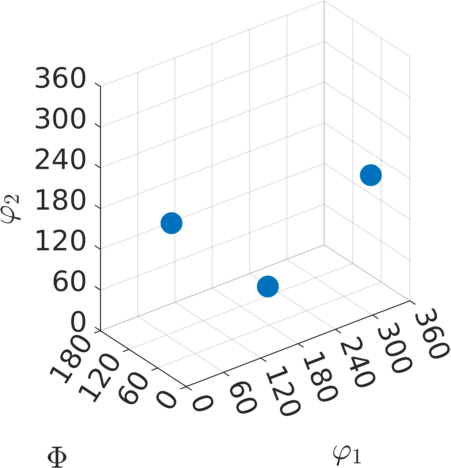
\includegraphics[width=0.8\textwidth]{pic/rotEuler}}

        \only<2>{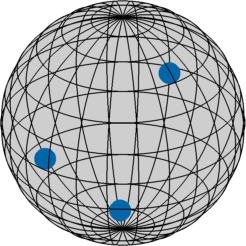
\includegraphics[width=0.8\textwidth]{pic/rotAxisAngle}}

        \only<3>{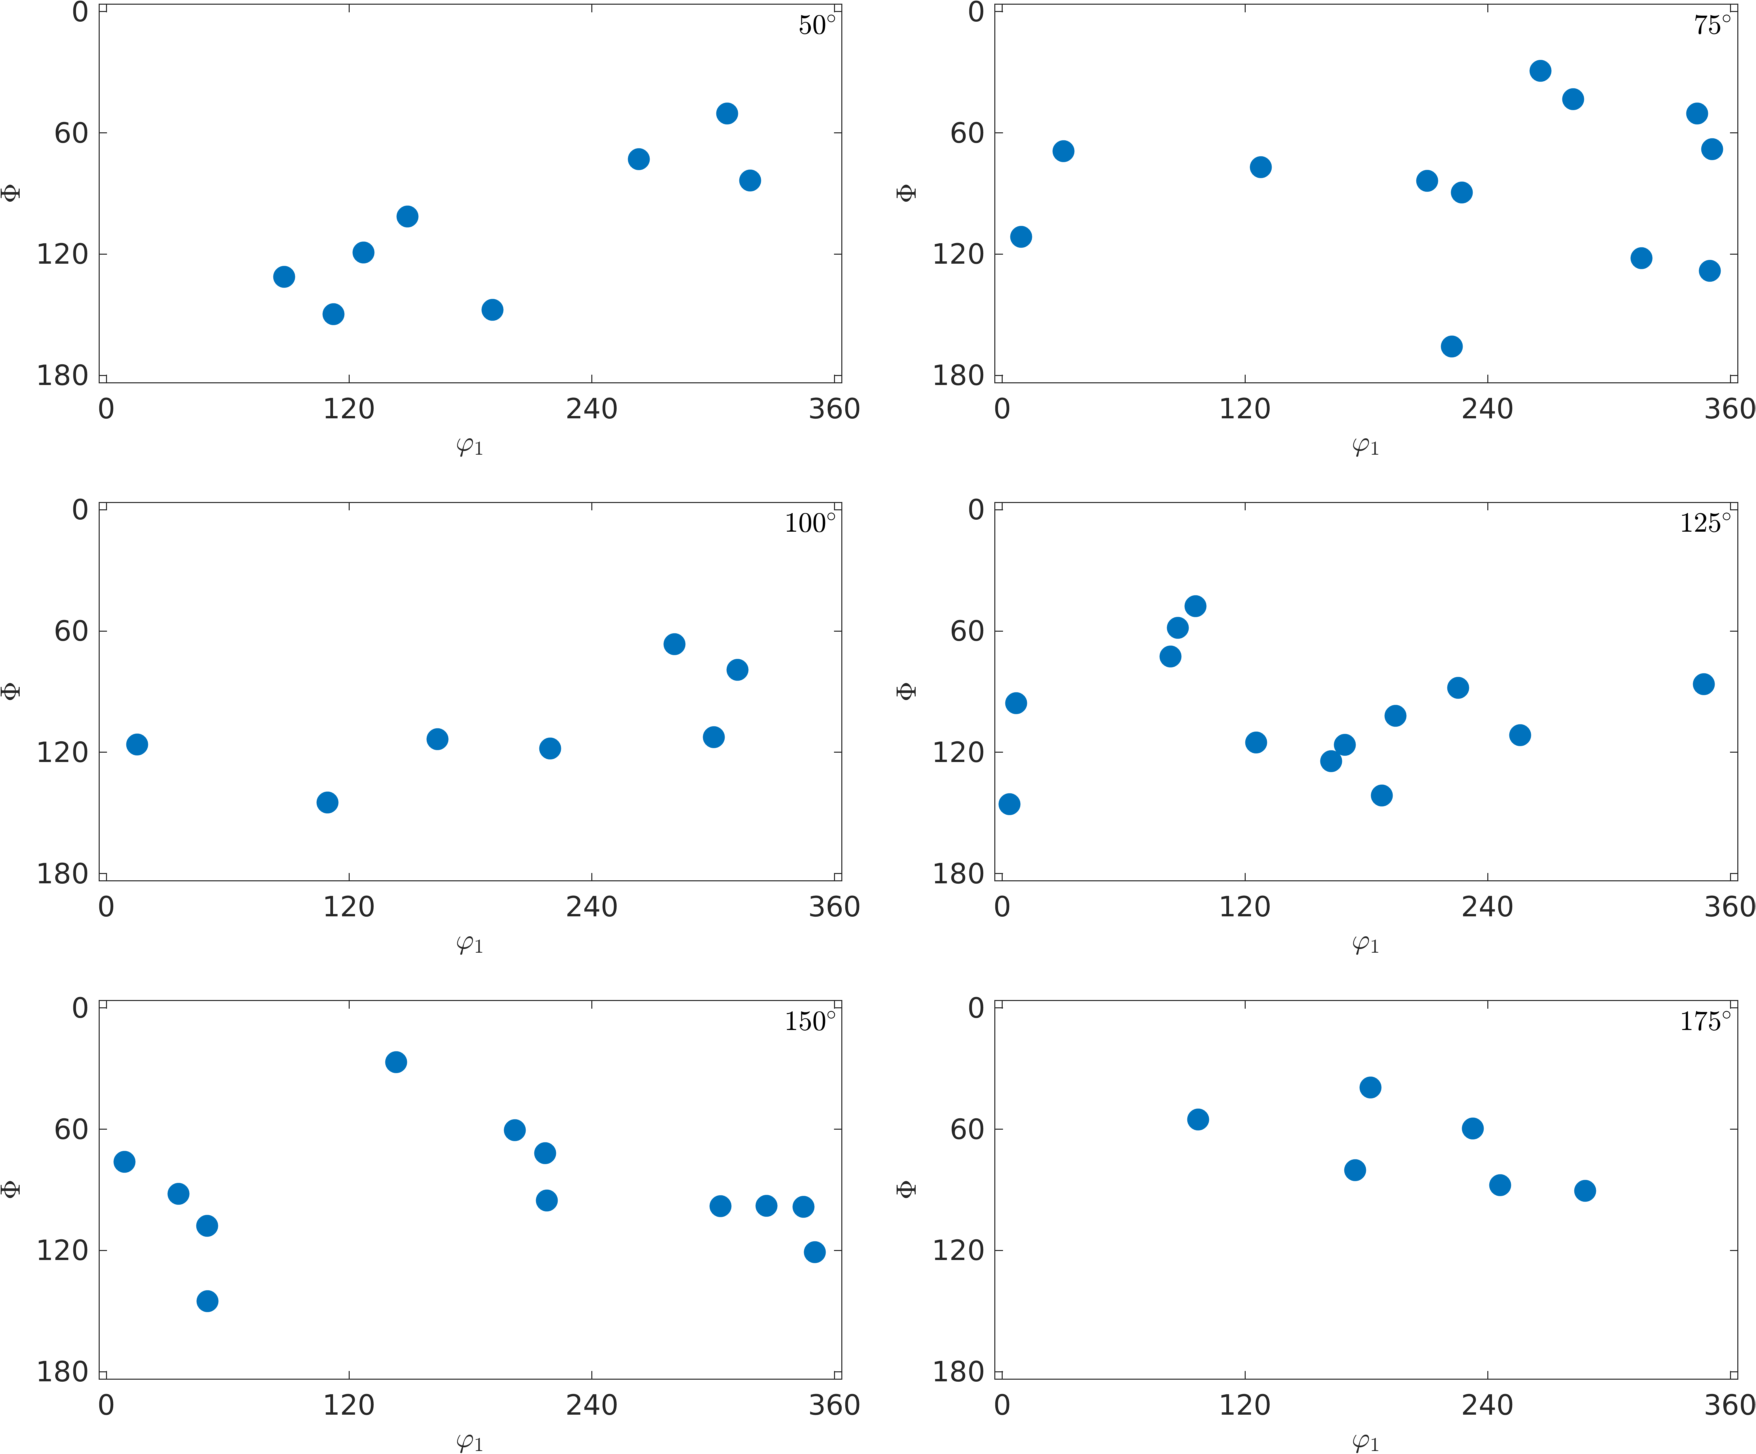
\includegraphics[width=\textwidth]{pic/rotEulerSec}}

        \only<4>{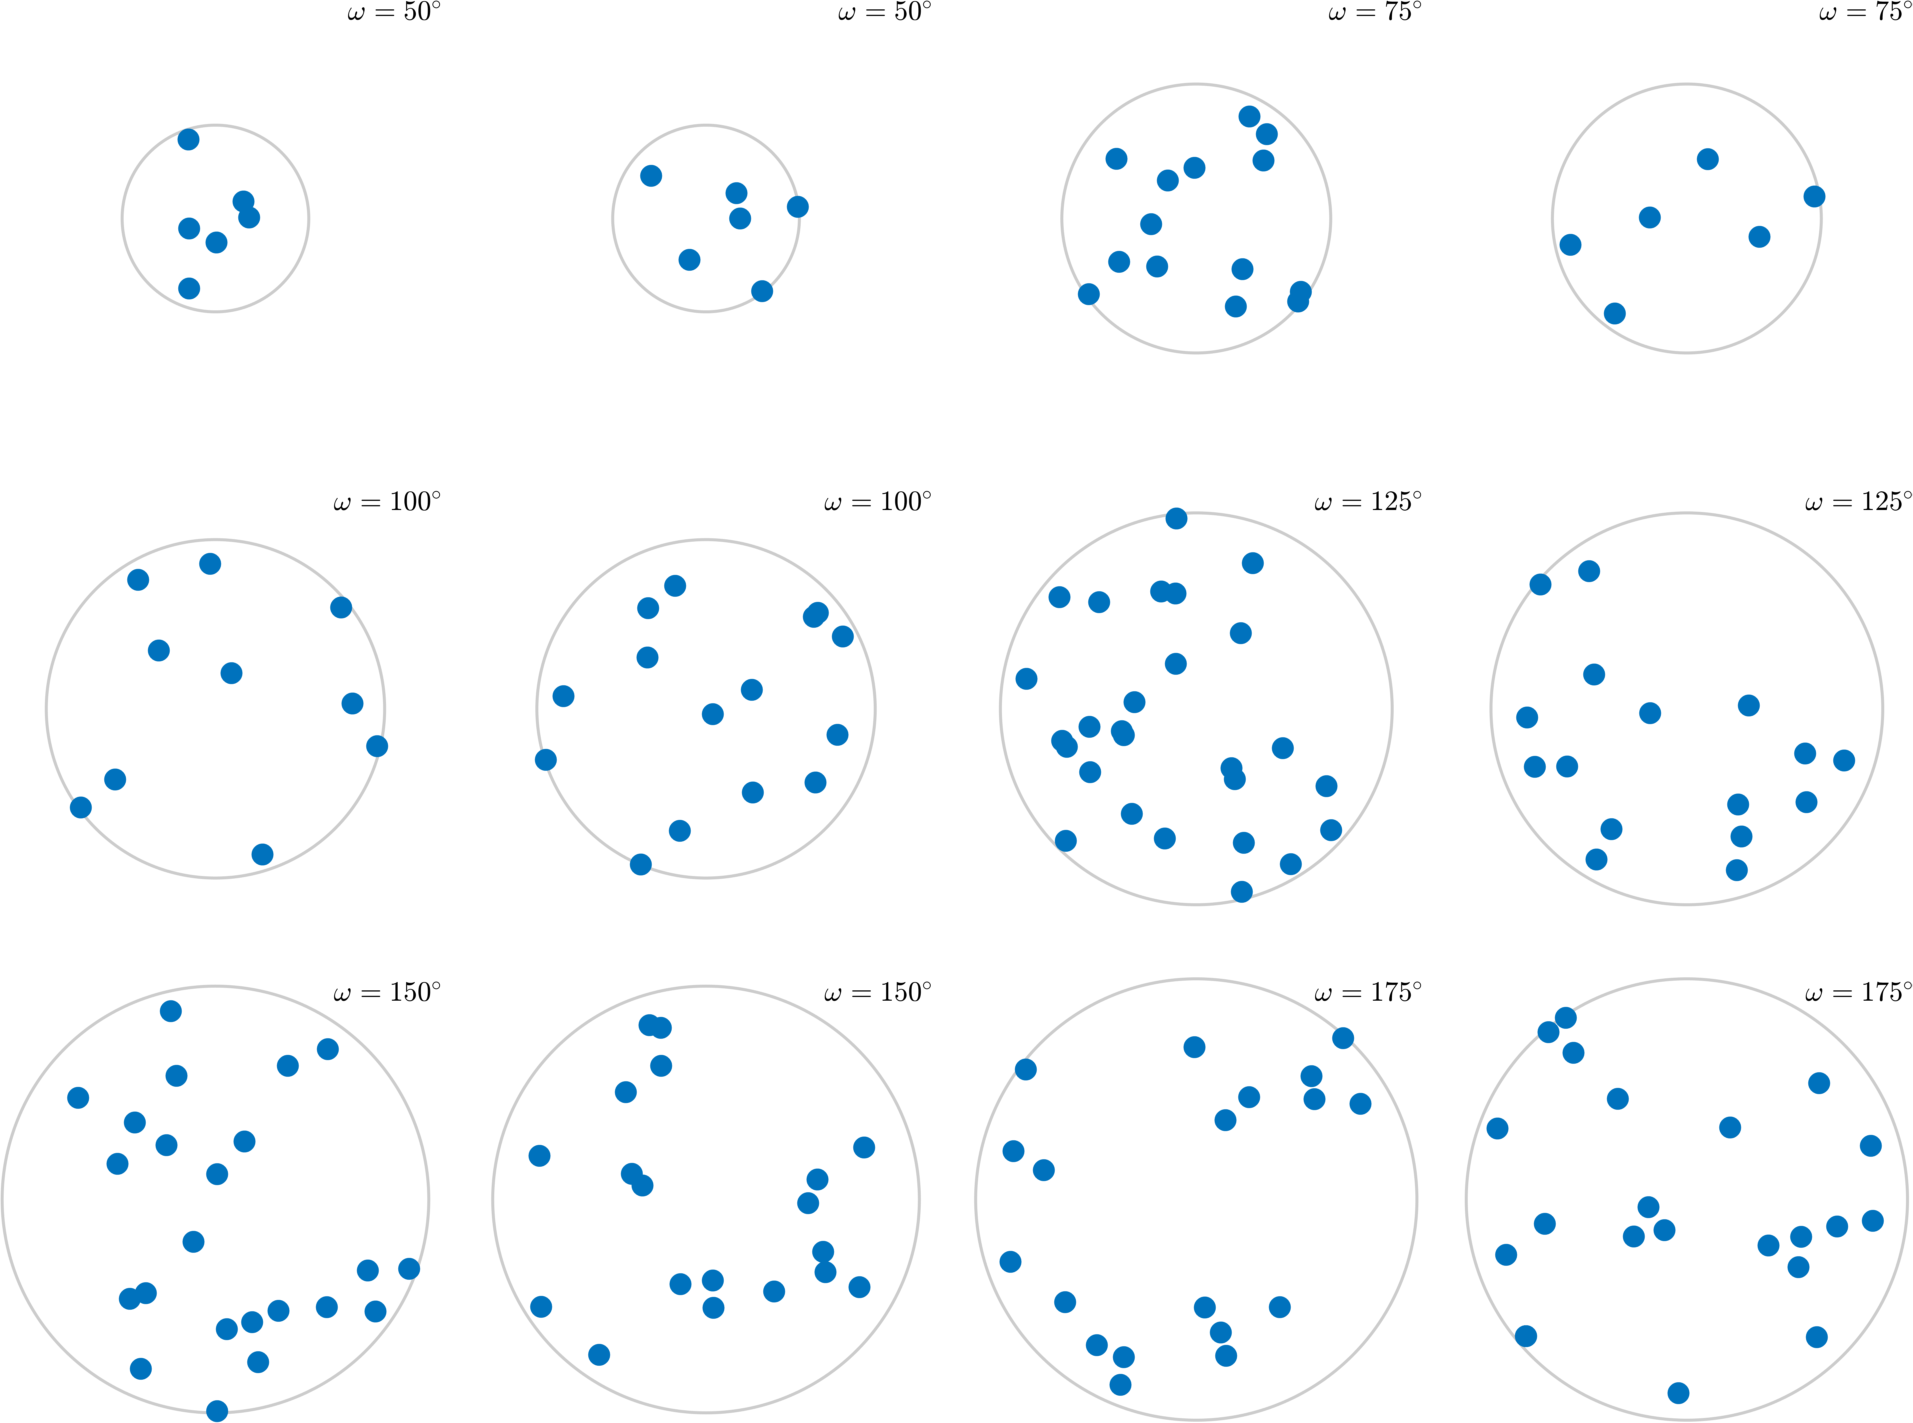
\includegraphics[width=\textwidth]{pic/rotAxisAngleSec}}


      \end{overlayarea}


    \end{column}

  \end{columns}


\end{frame}


\begin{frame}
  \frametitle{Summary of Rotation Representations}

      \begin{table}
  \centering
  \begin{tabular}{>{\centering\bfseries}m{1.5in} >{\centering}m{1in}  >{\centering}m{1.5in} >{\centering\arraybackslash}m{0.7in}}
    \toprule
    name
    & \textbf{notation}
    & \textbf{space}
    & \textbf{dimension}  \\
    \midrule
    matrix
    & $\mat R$
    & $\R^{3 \times 3}$
    & 9 \\[2ex]
    Euler angles
    & $(\varphi_{1},\Phi,\varphi_{2})$
    &$[0,2\pi]\times[0,\pi]\times[0,2\pi]$
    &  3 \\[2ex]
    quaternion
    & $(q_{1},q_{2},q_{3},q_{4})$
    & $\S^{4}$
    & 4 \\[2ex]
    Rodrigues - Frank
    & $\tan \tfrac{\omega}2 \vec v$
    & $\R^{3}$  & 3\\[2ex]
    axis angle & $\omega \vec v$  & $\mathbb B^3$ & 3 \\[2ex]
    Miller-Bravais Indices
    & $(hkl)[uvw]$
    & $\S^{2} \times \S^{2}$ & 6\\[2ex]
    \bottomrule
  \end{tabular}
\end{table}

\end{frame}


\begin{frame}[fragile]
  \frametitle{Symmetries}

  \begin{columns}[T,onlytextwidth]
    \begin{column}{0.66\textwidth}
      \vspace{-1cm}
      \begin{overlayarea}{\textwidth}{0.85\textheight}

        \begin{Definition}
          \begin{itemize}
          \item A crystal symmetry is a transformation (translation + \\rotation) that keeps the crystal
            lattice invariant.
          \item The group of all crystal symmetries is called \structure{space
              group}.
          \item Their rotational parts form the \structure{point group}.
          \end{itemize}
        \end{Definition}

        \medskip
  
        The symmetry elements in a point group are generated by
        \begin{itemize}
        \item rotations about 180, 120, 90 or 60 degrees
        \item reflections
        \item the inversion
        \end{itemize}
        \begin{onlyenv}<1>
        \begin{lstlisting}[style=input]
Z   = vector3d.Z
rot = rotation.byAxisAngle(Z,120*degree)
cs  = crystalSymmetry.byElements(rot)
\end{lstlisting}
\end{onlyenv}
\begin{onlyenv}<2->
\begin{lstlisting}[style=input]
Z   = vector3d.Z
rot = rotation.byAxisAngle(Z,120*degree)
m   = reflection(vector3d.X)
cs  = crystalSymmetry.byElements([rot, m])
\end{lstlisting}
\end{onlyenv}
\begin{onlyenv}<3->
  \begin{lstlisting}[style=input]
cs  = cs.add(rotation.inversion)
\end{lstlisting}
\end{onlyenv}
    

      \end{overlayarea}      
    \end{column}
    \begin{column}{0.29\textwidth}
      \vspace{-0.5cm}
      \begin{overlayarea}{\textwidth}{0.85\textheight}
        \centering
        \begin{onlyenv}<1> 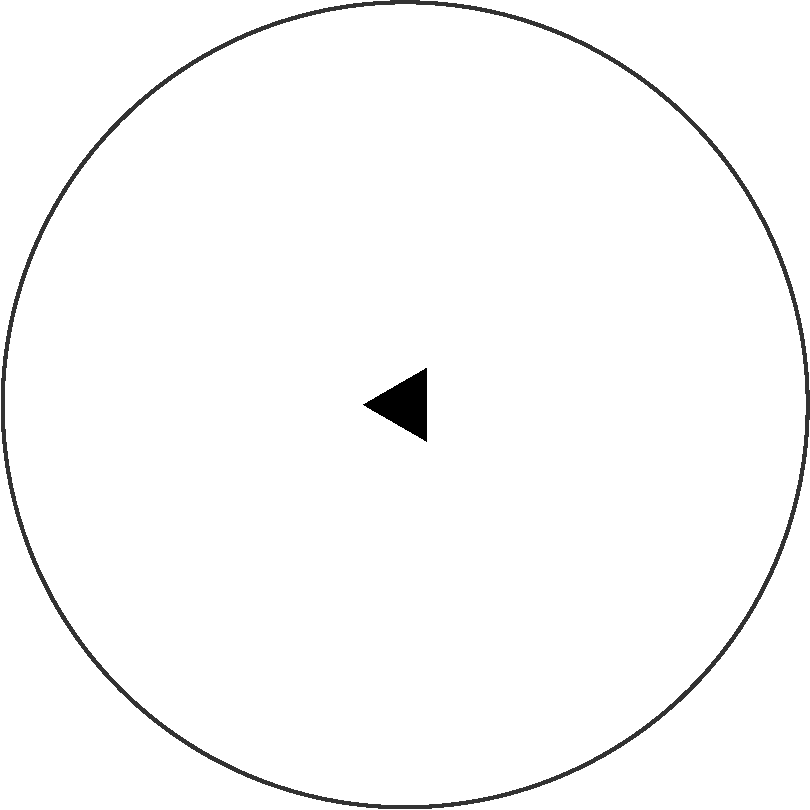
\includegraphics[width=\textwidth]{pic/Sym3}
        \end{onlyenv}
        \begin{onlyenv}<2> 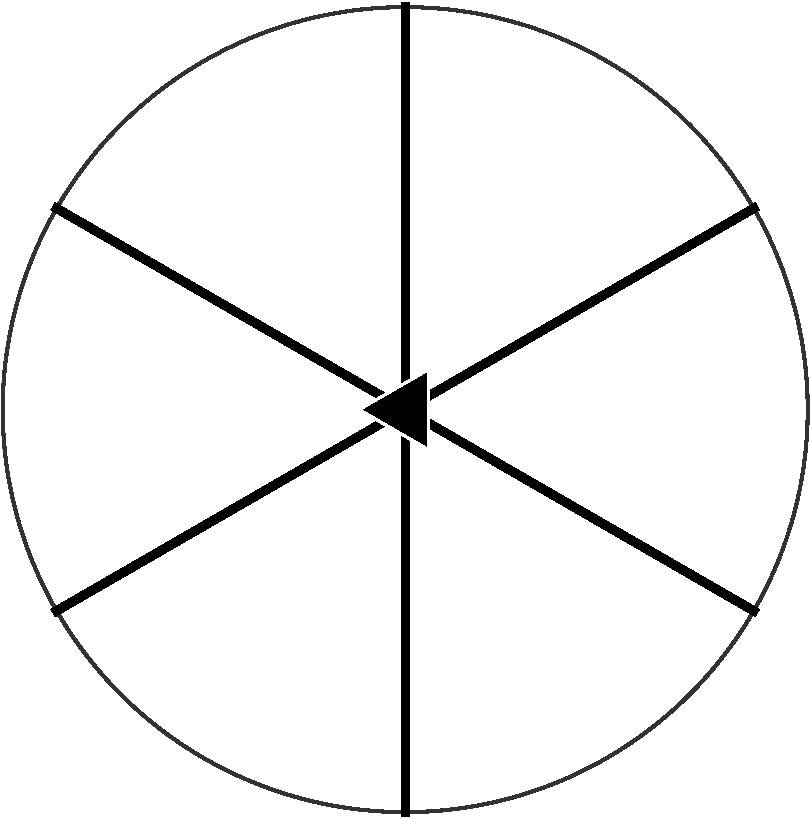
\includegraphics[width=\textwidth]{pic/Sym321}
        \end{onlyenv}
        \begin{onlyenv}<3-> 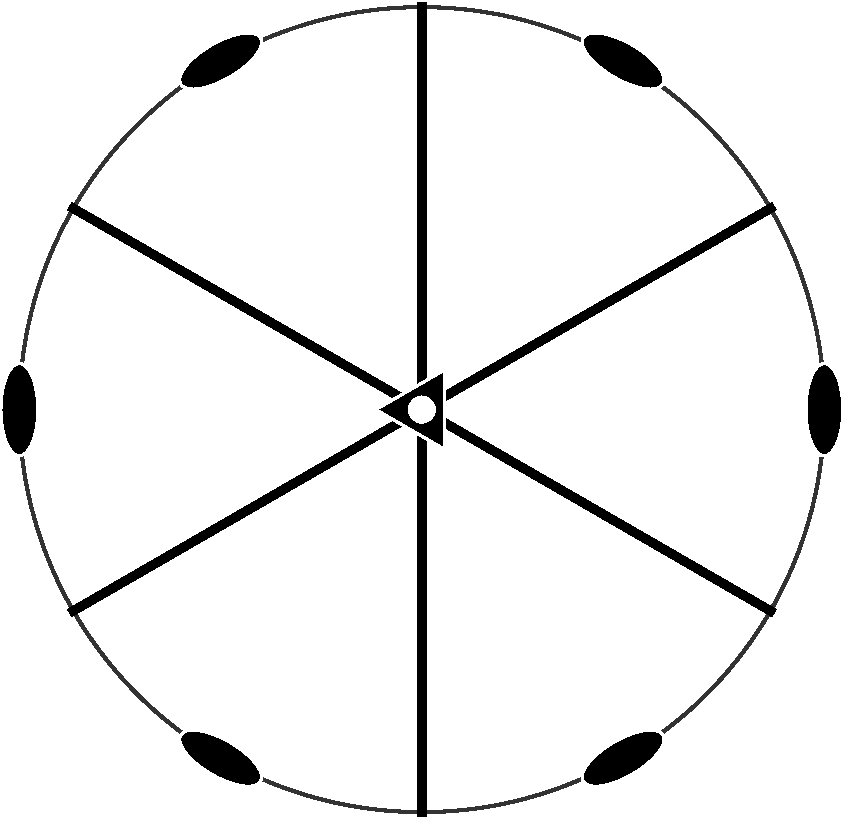
\includegraphics[width=\textwidth]{pic/Sym-3m}
        \end{onlyenv}
        \begin{onlyenv}<4> 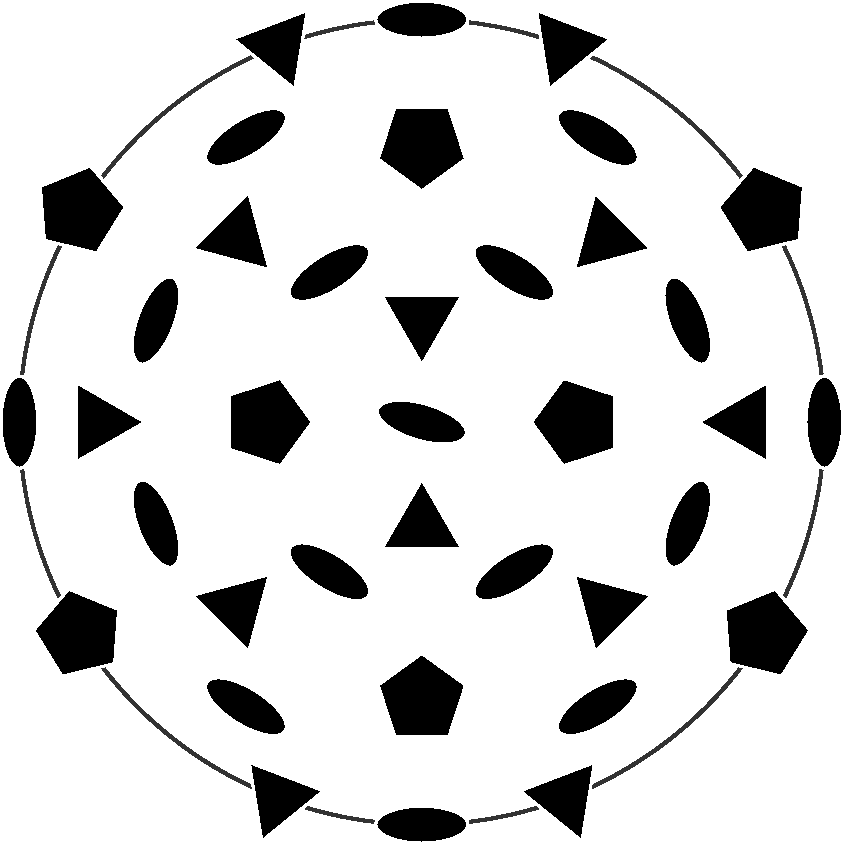
\includegraphics[width=\textwidth]{pic/Sym532}
        \end{onlyenv}
     \end{overlayarea}

    \end{column}
  \end{columns}

\end{frame}

% \begin{frame}
%   \frametitle{Affine Transformations}

%   \begin{Definition}
%     \structure{Affine transformations} are transformations
%     \begin{equation*}
%       \mat S(\vec x) = \mat R \vec x + \vec t
%     \end{equation*}
%     that are compositions of a rotation $\mat R \in O(3)$ and a translation
%     $\vec t \in \R^{3}$.

%     \medskip

%     The set of all affine transformations in the three dimensional space is
%     called \structure{Euclidean motion group} and is denoted by
%     \structure{$\mathrm{SE} (3)$}.
%   \end{Definition}

%   \bigskip
%   \pause

%   Let $\mat S_{1}(\vec x) = \mat R_{1} \vec x + \vec t_{1}$ and $\mat
%   S_{1}(\vec x) = \mat R_{1} \vec x + \vec t_{1}$ be two affine
%   transformations. Then their composition
%   \begin{equation*}
%     \mat S_{2} \circ \mat S_{1} (\vec x)
%     = \mat S_{2}(\mat S_{1}(\vec x))
%     = \mat R_{2} \mat R_{1} \vec x + \mat R_{2} \vec t_{1} + \vec t_{2}
%   \end{equation*}
%   is again an affine transformation.

% \end{frame}


% \begin{frame}
%   \frametitle{The Eucledean Motion Group}

%   The affine transformations, together with the composition operation $\circ$,
%   define a group, i.e., the satisfy the following conditions:
%   \begin{enumerate}
%   \item For any three affine transformations $\mat S_{1}, \mat S_{2}, \mat
%     S_{3} \in SE(3)$ it holds
%     \begin{equation*}
%       (\mat S_{1} \circ \mat S_{2}) \circ \mat S_{3}
%       =  (\mat S_{1} \circ \mat S_{2} \circ \mat S_{3})
%     \end{equation*}
%   \item There is an identical affine transformation $\mat S_{id}(\vec x) = \vec x$ such that
%     \begin{equation*}
%       \mat S_{id} \circ \mat S = \mat S \circ \mat S_{id} = \mat S.
%     \end{equation*}
%   \item For every affine transformation $\mat S(\vec x) = \mat R \vec x + \vec
%     t$ there is an inverse transformation
%     \begin{equation*}
%       \mat S^{-1}(\vec x) = \mat R^{-1} \vec x - \mat R^{-1} \vec t
%     \end{equation*}
%     such that
%     \begin{equation*}
%       \mat S^{-1} \circ \mat S = \mat S \circ \mat S^{-1} = \mat S_{id}.
%     \end{equation*}
%   \end{enumerate}


% \end{frame}

% \begin{frame}
%   \frametitle{Crystal Symmetries}

%   \begin{Definition}
%     The subset $\mathcal E \subset \mathrm{SE}(3)$ off all affine transformations that
%     keep the atom lattice invariant is called \structure{space group} of the
%     crystal.
%   \end{Definition}

%   The space group $\mathcal S$ together with the composition $\circ$ is a
%   group, since for any two symmetries $\mat S_{1}, \mat S_{2} \in \mathcal E$
%   we have $\mat S_{1} \circ \mat S_{2} \in \mathcal E$.

%   \pause

%   \begin{Definition}
%     Let $\mat S_{1}, \ldots, \mat S_{n} \in SE(3)$ arbitrary affine
%     transformations. Then we denote by
%     \structure{$\left<\mat S_{1}, \ldots, \mat S_{n}\right>$} the smallest
%     subgroup of $SE(3)$ that contains the transformations
%     $\mat S_{1}, \ldots, \mat S_{n}$ and call it the \structure{group
%       generated by $\mat S_{1}, \ldots, \mat S_{n}$}.
%   \end{Definition}

%   \begin{exampleblock}{Example}
%     The group generated by the rotation $\mat R_{\vec z,120^{\circ}}$ about
%     $120^{\circ}$ about the z-axis is
%     \begin{equation*}
%       \left< \mat R_{\vec z,120^{\circ}} \right>
%       = \{ \mat R_{\vec z,120^{\circ}},
%       \mat R_{\vec z,120^{\circ}}^{2}, \mat R_{\vec z,120^{\circ}}^{3} \}
%       = \{ \mat R_{\vec z,0^{\circ}},
%       \mat R_{\vec z,120^{\circ}}, \mat R_{\vec z,240^{\circ}} \}
%     \end{equation*}
%   \end{exampleblock}
% \end{frame}

% \begin{frame}[fragile]
%   \frametitle{Generate Point Groups in MTEX}

%   \begin{columns}[T,onlytextwidth]
%     \begin{column}{0.63\textwidth}
%       \vspace{-1cm}
%       \begin{overlayarea}{\textwidth}{0.85\textheight}
%       \begin{lstlisting}[style=input]
% Z   = vector3d.Z
% rot = rotation.byAxisAngle(Z,120*degree)
% cs  = crystalSymmetry.byElements(rot)
% \end{lstlisting}
% \begin{onlyenv}<1>
%   \vspace{-0.4cm}
%   \begin{lstlisting}[style=output]
% cs.rot = /+rotation+/
%   size: 3 x 1

%   Bunge Euler angles in degree
%   phi1  Phi phi2 Inv.
%    240    0    0    0
%    120    0    0    0
%      0    0    0    0
%   \end{lstlisting}
% \end{onlyenv}

% \medskip
% \begin{onlyenv}<2->
%       add some mirroring \vspace{-0.2cm}
%       \begin{lstlisting}[style=input]
% m  = reflection(vector3d.X)
% cs = crystalSymmetry.byElements([rot, m])
% \end{lstlisting}
% \end{onlyenv}
% \begin{onlyenv}<2>
%   \vspace{-0.4cm}
%   \begin{lstlisting}[style=output]
% cs.rot = /+rotation+/
%   size: 6 x 1

%   Bunge Euler angles in degree
%   phi1  Phi phi2 Inv.
%    240  180    0    1
%      0  180  240    1
%    120  180  120    1
%    240    0    0    0
%    120    0    0    0
%      0    0    0    0
%   \end{lstlisting}
% \end{onlyenv}

%       \medskip

% \begin{onlyenv}<3->
%       add the inversion \vspace{-0.2cm}
%       \begin{lstlisting}[style=input]
% cs = cs.add(rotation.inversion)
%       \end{lstlisting}
%     \end{onlyenv}
% \begin{onlyenv}<3>
%   \vspace{-0.4cm}
%   \begin{lstlisting}[style=output]
% cs = /+crystalSymmetry+/

%   symmetry       : -3m1
%   elements       : 12
%   a, b, c        : 1, 1, 1
%   reference frame: X||a, Y||b, Z||c
% \end{lstlisting}
% \end{onlyenv}

% \medskip

% \begin{onlyenv}<4->
%       some quasi symmetry \vspace{-0.2cm}
% \begin{lstlisting}[style=input]
% r2 = rotation.byAxisAngle(Z, 180*degree)
% a5 = vector3d.byPolar(31.7171*degree, 0)
% r5 = rotation.byAxisAngle(a5, 72*degree)
% cs = crystalSymmetry.byElements([r2, r5])
% \end{lstlisting}
% \end{onlyenv}
% \end{overlayarea}
% \end{column}
%     \begin{column}{0.34\textwidth}

% %      \begin{overlayarea}{\textwidth}{0.85\textheight}
%         \centering
%         \begin{onlyenv}<1> 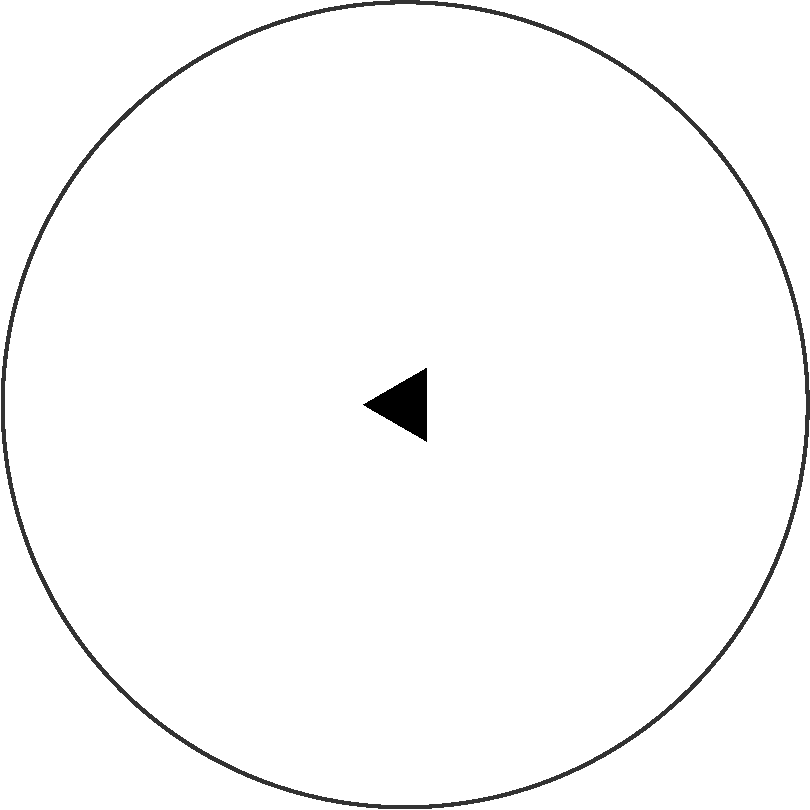
\includegraphics[width=\textwidth]{pic/Sym3}
%         \end{onlyenv}
%         \begin{onlyenv}<2> 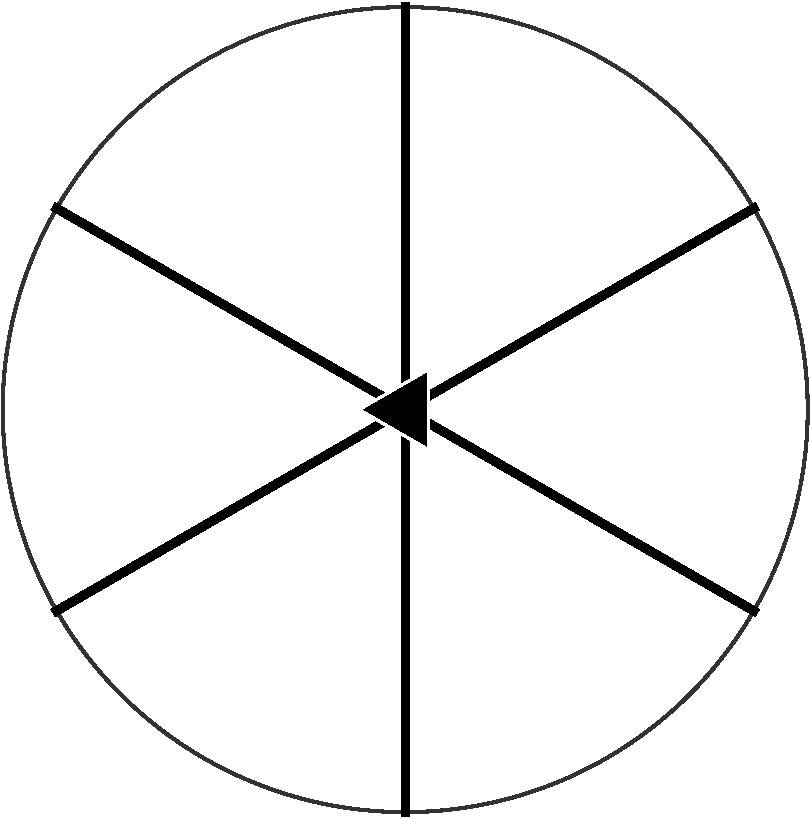
\includegraphics[width=\textwidth]{pic/Sym321}
%         \end{onlyenv}
%         \begin{onlyenv}<3> 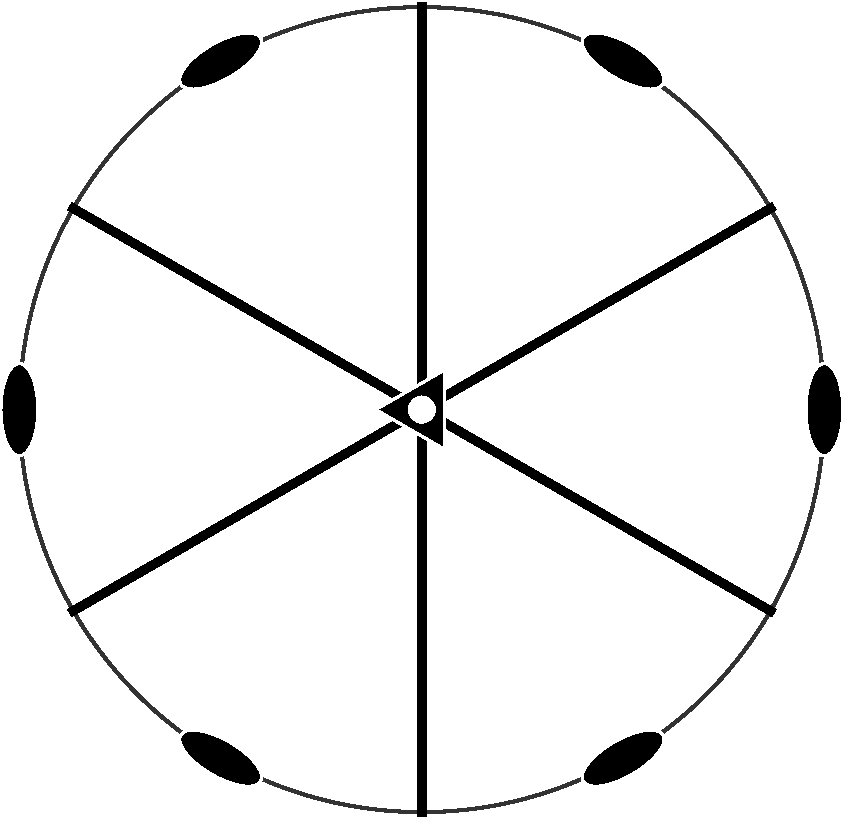
\includegraphics[width=\textwidth]{pic/Sym-3m}
%         \end{onlyenv}
%         \begin{onlyenv}<4> 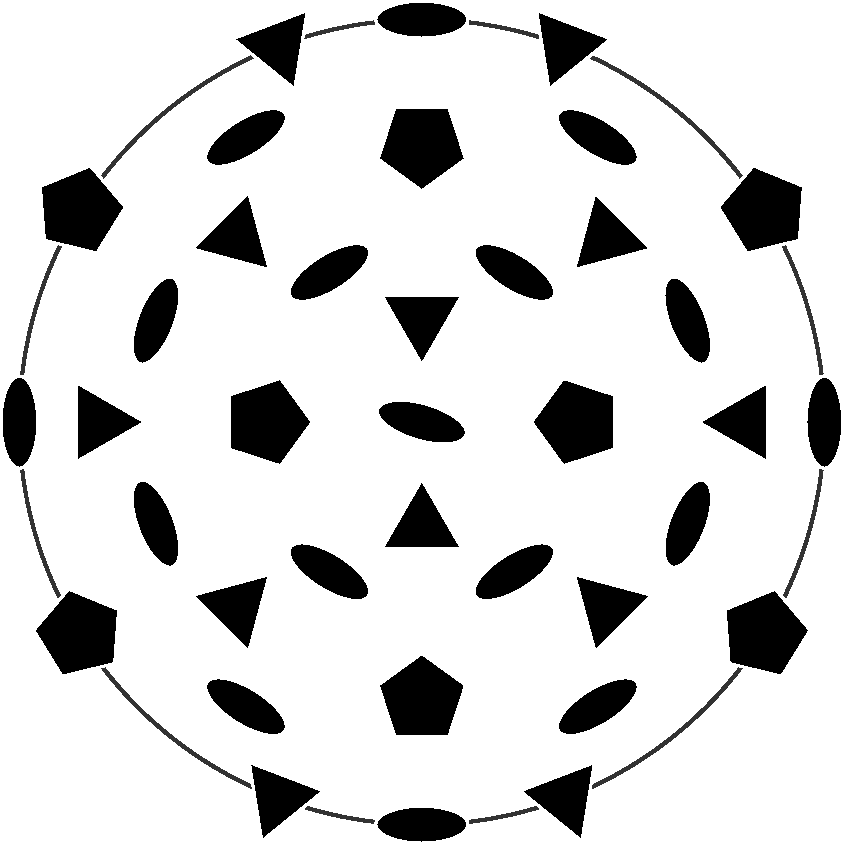
\includegraphics[width=\textwidth]{pic/Sym532}
%         \end{onlyenv}
%  %     \end{overlayarea}

%     \end{column}
%   \end{columns}
% \end{frame}


% \begin{frame}
%   \frametitle{Point Groups}

%   \begin{Definition}
%     Let
%     $\mathcal E = \{(\mat R_{1},\vec t_{1}),(\mat R_{2},\vec t_{2}),\ldots \}$
%     be the space group of a crystal structure. Then
%     $\mathcal P = \{\mat R_{1}, \mat R_{2},\ldots\}$ is a subgroup of $O(3)$
%     and called the \structure{point group} of the crystal structure.
%   \end{Definition}

%   \begin{itemize}
%   \item The space group describes the symmetries of an infinite periodic crystal
%     lattice.
%   \item The point group describes the symmetries of the finite unit cell.
%   \end{itemize}

%   \pause

%   \begin{block}{Goal:}
%     Characterize and describe all possible space groups $\mathcal E$ and all
%     possible point groups $\mathcal P$.
%   \end{block}


%   \pause

%   \begin{alertblock}{Result:}
%     There are exactly 230 different space groups and 32 different point groups.
%   \end{alertblock}


% \end{frame}


% \begin{frame}
%   \frametitle{Symmetry Operations}


%   \begin{table}
%   \begin{center}
%     \begin{tabular}{lrrr}
%       \toprule
%       name
%       & \makecell[tr]{affine\\transformation}
%       & \makecell[tr]{Hermann–Mauguin\\symbol}
%       & \makecell[tr]{graphical\\symbol}\\
%       \midrule
%       rotational axis
%       & $\mat R_{\vec d,\frac{360^{\circ}}n}$
%       & $2$, $3$, $4$ ,$6$
%       & \tikz \fill[black] (0,0) ellipse[x radius=2pt, y radius=5pt,
%         fill=black];
%         \tikz \node[draw=black,fill=black,isosceles
%         triangle,isosceles triangle stretches,shape border rotate=90,minimum
%         width=10pt,minimum height=10pt,inner sep=0pt] at (0,0) {};
%         \tikz \node[draw=black,fill=black,rectangle,shape border rotate=90,minimum
%         width=10pt,minimum height=10pt,inner sep=0pt] at (0,0) {};
%         \tikz \node[draw=black,fill=black,regular polygon, regular polygon sides=6,
%         minimum width=12pt,minimum height=12pt,inner sep=0pt] at (0,0) {};\\
%       inversion
%       & $-\mat I$
%       & $\overline{1}$
%       & \tikz \draw[very thick] (0,0) circle[radius = 2pt];\\
%       mirror plane
%       & $-\mat R_{\vec n,180}$
%       & $m=\overline{2}$
%       & \tikz \draw[thick] (0,0) -- (0,10pt);\\
%       rotoinversion axis
%       & $-\mat R_{\vec d,\frac{360^{\circ}}n}$
%       & $\overline{3}$, $\overline{4}$, $\overline{6}$
%       & \tikz{ \node[draw=black,fill=black,isosceles
%         triangle,isosceles triangle stretches,shape border rotate=90,minimum
%         width=10pt,minimum height=10pt,inner sep=0pt] at (0,0) {};
%         \draw[black,fill=white] (0,0) circle[radius=2pt];}
%         \tikz{\node[very thick,draw=black,rectangle,shape border rotate=90,minimum
%         width=10pt,minimum height=10pt] at (0,0) {};
%         \draw[rotate=45, fill=black,scale=1.1] (0,0) ellipse[x radius=2pt, y radius=5pt];
%         }
%         \tikz{\node[very thick,draw=black,regular polygon, regular polygon sides=6,
%         ,shape border rotate=90,minimum width=12pt,minimum height=12pt,inner sep=0pt] at (0,0) {};
%         \node[draw=black,fill=black,isosceles
%         triangle,isosceles triangle stretches,shape border rotate=90,minimum
%         width=8pt,minimum height=8pt,inner sep=0pt] at (0,-0.5pt) {};
%         }\\
%       translation
%       & $\vec t$ \\
%       screw axis
%       & $\mat R_{\vec d,\frac{360^{\circ}}n} + \vec d$
%       &  \makecell[tr]{$2_{1}$, $3_{1}$,  $3_{2}$, $4_{1}$,$4_{2}$,$4_{3}$\\
%       $6_{1}$,$6_{2}$,$6_{3}$,$6_{4}$,$6_{5}$}\\
%       glide plane
%       & $-\mat R_{\vec d,\frac{180^{\circ}}n} + \vec d$
%       & $a$, $b$, $c$, $n$, $d$
%       &\\
%       \bottomrule
%     \end{tabular}
%   \end{center}
% \end{table}
% \end{frame}


% \begin{frame}
%   \frametitle{Cyclic Groups}

%   \begin{itemize}
%  \item $\mat S \in \mathcal P$ $\implies$
%     $\mat S^{n} \in \mathcal P$, for all $n \in \mathbb Z$
%   \item $\mat R_{\vec d, \frac{1}{m} 360^{\circ}} \in \mathcal P$ $\implies$
%     $\mat R_{\vec d, \frac{n}{m} 360^{\circ}} \in \mathcal P$, $n =
%     0,\ldots,m-1$.
%   \item Only rotational axes of order $2$, $3$, $4$, $6$ are compatible with
%     periodic lattices
%   \end{itemize}

%   \bigskip

%   \setlength{\tabcolsep}{2pt}
%   \begin{tabular}{ccccc}
%      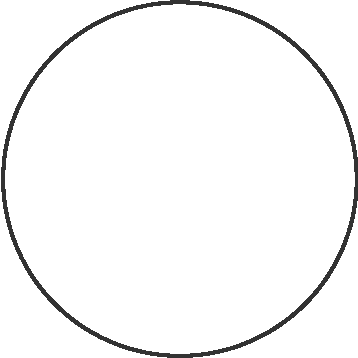
\includegraphics[width=0.19\textwidth]{symmetries/1.pdf}
%      &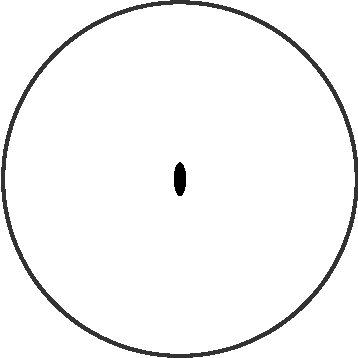
\includegraphics[width=0.19\textwidth]{symmetries/9.pdf}
%      &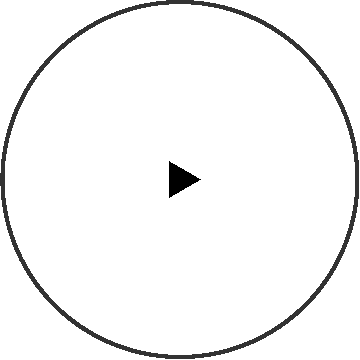
\includegraphics[width=0.19\textwidth]{symmetries/17.pdf}
%      &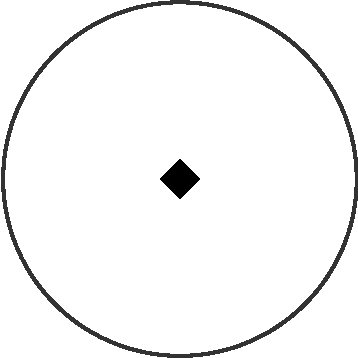
\includegraphics[width=0.19\textwidth]{symmetries/25.pdf}
%      &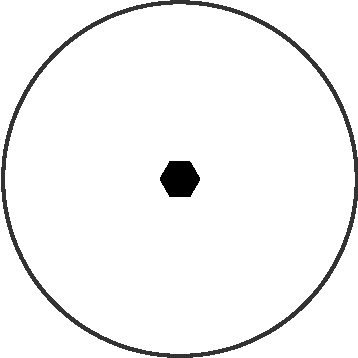
\includegraphics[width=0.19\textwidth]{symmetries/33.pdf}\\
%      1 & 2 & 3 & 4 & 6\\
%      $C_{1}$ &    $C_{2}$ &    $C_{3}$ &    $C_{4}$ &    $C_{6}$
%    \end{tabular}
% \end{frame}


% \begin{frame}
%   \frametitle{Dieder Groups}

%   Two two fold symmetry axis $\vec a$, $\vec b$ at an angle generate a
%   perpendicular symmetry axis

%   \begin{itemize}
%   \item $\mat R_{\vec a, \pi}, \mat R_{\vec b, \pi} \in \mathcal P$,
%     $\angle(\vec a,\vec b) = \frac{\pi}{n}$
%     $\implies$ $\mat R_{\vec a \times \vec b, \frac{2\pi}n} \in \mathcal P$
%   \end{itemize}

%   \setlength{\tabcolsep}{2pt}
%   \begin{tabular}{ccccc}
%     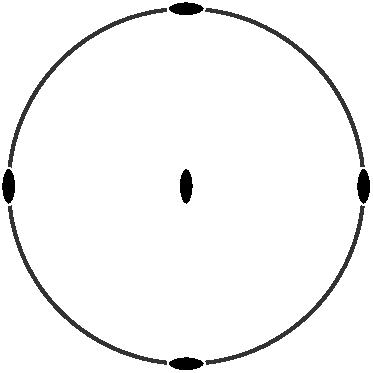
\includegraphics[width=0.19\textwidth]{symmetries/12.pdf}
%     &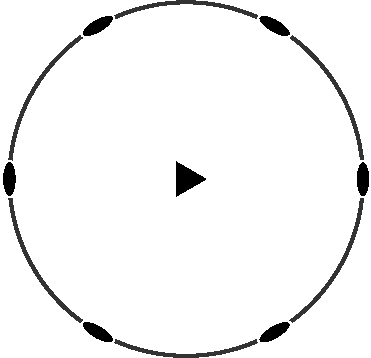
\includegraphics[width=0.19\textwidth]{symmetries/19.pdf}
%     &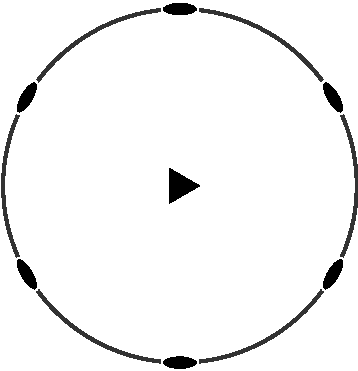
\includegraphics[width=0.19\textwidth]{symmetries/22.pdf}
%     &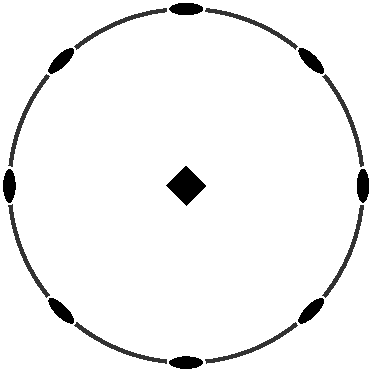
\includegraphics[width=0.19\textwidth]{symmetries/28.pdf}
%     &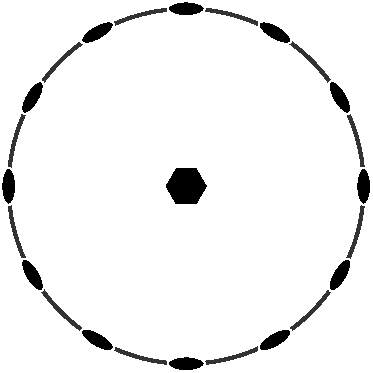
\includegraphics[width=0.19\textwidth]{symmetries/36.pdf}\\
%     222 & 321 & 312 & 422 & 622\\
%     $D_{2}$ &    $D_{3}$ & $D_3$ &   $D_{4}$ &    $D_{6}$
%   \end{tabular}

% \end{frame}


% \begin{frame}
%   \frametitle{Tetragonal and Cubic Symmetry}


%   \begin{columns}
%     \begin{column}{0.8\textwidth}
%       \begin{itemize}
%       \item $\vec a$ - $m$-fold symmetry axis, $m>2$
%       \item $\vec b$ - $n$-fold symmetry axis
%       \item $\implies$ $\mat R_{\vec a,\frac{k}{m}2\pi} \vec b$,
%         $k=1,\ldots,m$ are $n$-fold symmetry axes
%       \item $\implies$ $\mat R_{\vec b,\frac{k}{n}2\pi} \vec a$,
%         $k=1,\ldots,n$ are $m$-fold symmetry axes
%       \item $\implies$ $\mat R_{\vec b,\frac{2k+1}{2n}2\pi} \vec a$,
%         $k=0,\ldots,n$ are $2$-fold symmetry axes
%       \item assume $\vec a$, $\vec b$ have  minimum angle in $\mathcal P$
%       \item $\implies$ $\mat R_{\vec a,\frac{k}{m}2\pi} \vec b$,
%         $k=1,\ldots,m$ form a regular spherical polygon
%         $P_{\vec a}$
%         % \item $\implies$ $\mat R_{\vec b,\frac{k}{n}2\pi} \vec b$,
%         %   $k=1,\ldots,n$
%         %   are the vertices of a a regular spherical polygon $P_{\vec b}$
%       \item applying all symmetry operations of $\mathcal P$ to $P_{\vec a}$
%         will cover the whole sphere by disjoint copies of $P_{\vec a}$
%       \item $\implies$ the copies of $P_{\vec a}$ form a Platonic solid
%       \item $\implies$ only tetrahedron and cube (octahedron) are relevant
%       \end{itemize}
%     \end{column}
%     \begin{column}{0.2\textwidth}

%       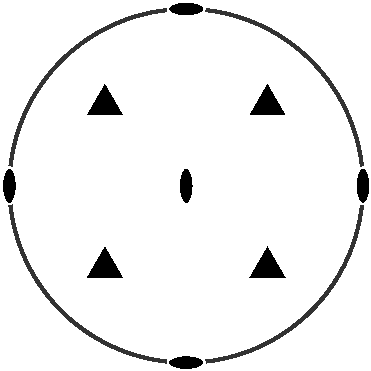
\includegraphics[width=\textwidth]{symmetries/41.pdf}
%       \vspace{-0.7cm}
%       \begin{center}
%         23 ($T$)\\
%       \end{center}
%       \medskip
%       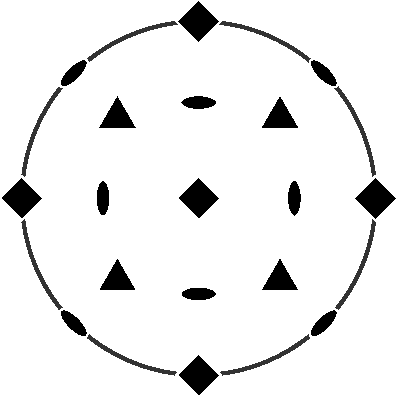
\includegraphics[width=\textwidth]{symmetries/43.pdf}
%       \vspace{-0.7cm}
%       \begin{center}
%         432 $(O)$
%       \end{center}

%     \end{column}
%   \end{columns}

% \end{frame}


\begin{frame}
  \frametitle{All 11 Enantiomorphic Symmetry Groups}

  \begin{center}
    \setlength{\tabcolsep}{2pt}
    \begin{tabular}{c|c|c|c|c|c|}
      \hline
      \multicolumn{1}{|c|}{triclinic}
      & monoclinic
      & trigonal
      & tetragonal
      & hexagonal
      & cubic\\
      \multicolumn{1}{|c|}{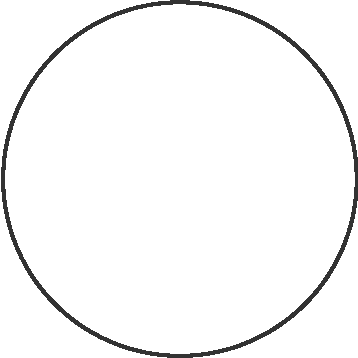
\includegraphics[width=0.155\textwidth]{symmetries/1.pdf}}
      &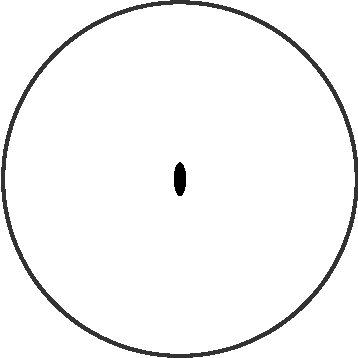
\includegraphics[width=0.155\textwidth]{symmetries/9.pdf}
      &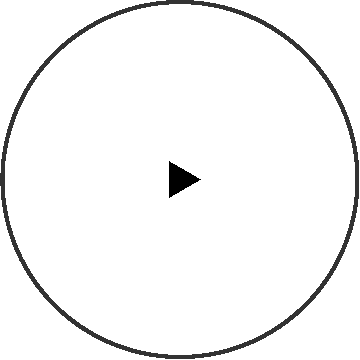
\includegraphics[width=0.155\textwidth]{symmetries/17.pdf}
      &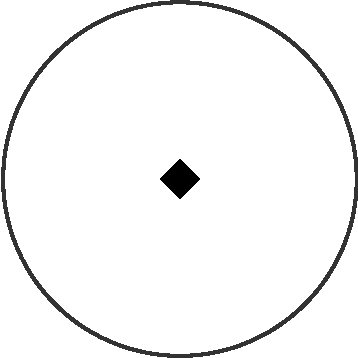
\includegraphics[width=0.155\textwidth]{symmetries/25.pdf}
      &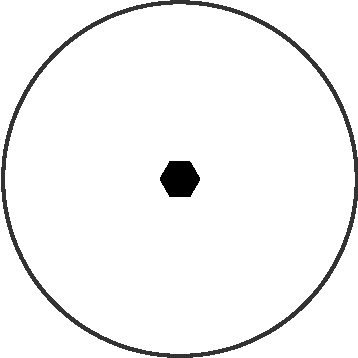
\includegraphics[width=0.155\textwidth]{symmetries/33.pdf}
      &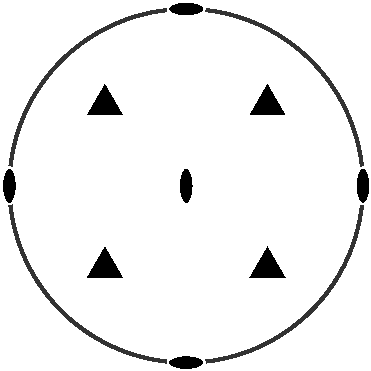
\includegraphics[width=0.155\textwidth]{symmetries/41.pdf}\\
      \multicolumn{1}{|c|}{1 $(\mathrm C_{1})$}
      & 2 $(\mathrm C_{2})$
      & 3 $(\mathrm C_{3})$
      & 4 $(\mathrm C_{4})$
      & 6 $(\mathrm C_{6})$
      & 23 $(\mathrm T)$ \\[1ex]
      \cline{1-2} %& 1 & 1 & & &\\
      &  orthorhombic & & & &\\
      &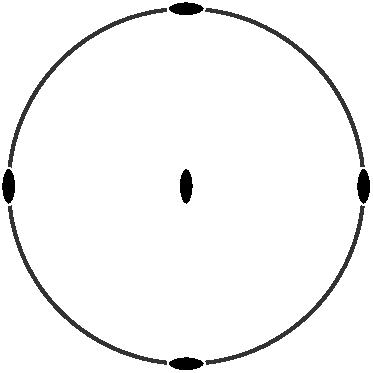
\includegraphics[width=0.155\textwidth]{symmetries/12.pdf}
      &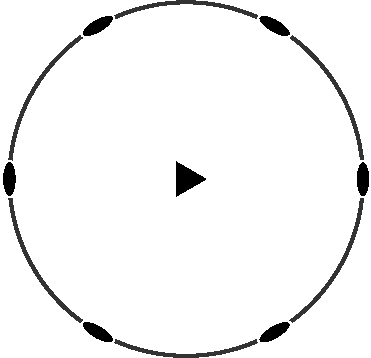
\includegraphics[width=0.155\textwidth]{symmetries/19.pdf}
      &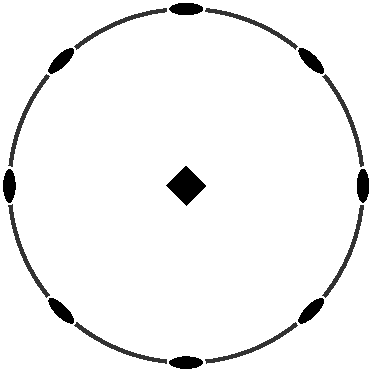
\includegraphics[width=0.155\textwidth]{symmetries/28.pdf}
      &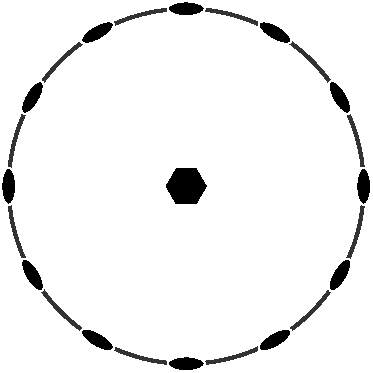
\includegraphics[width=0.155\textwidth]{symmetries/36.pdf}
      &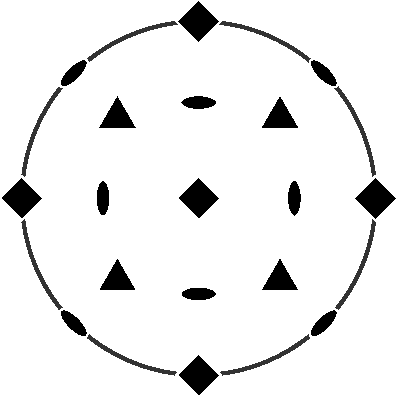
\includegraphics[width=0.155\textwidth]{symmetries/43.pdf}\\
      & 222 $(\mathrm D_{2})$
      & 321 $(\mathrm D_{3})$
      & 422 $(\mathrm D_{4})$
      & 622 $(\mathrm D_{6})$
      & 432 $(\mathrm O)$\\
      \cline{2-6}
    \end{tabular}
  \end{center}
\end{frame}


\begin{frame}
  \frametitle{All 11 Laue Symmetry Groups}

  \begin{center}
    \setlength{\tabcolsep}{2pt}
    \begin{tabular}{c|c|c|c|c|c|}
      \hline
      \multicolumn{1}{|c|}{triclinic}
      & monoclinic
      & trigonal
      & tetragonal
      & hexagonal
      & cubic\\
      \multicolumn{1}{|c|}{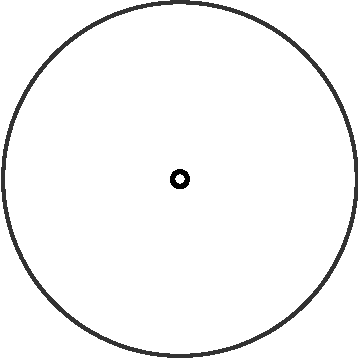
\includegraphics[width=0.155\textwidth]{symmetries/2.pdf}}
      &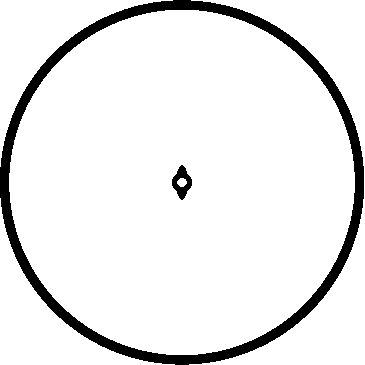
\includegraphics[width=0.155\textwidth]{symmetries/11.pdf}
      &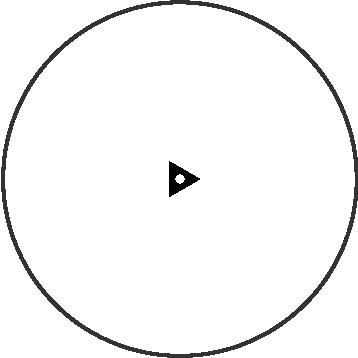
\includegraphics[width=0.155\textwidth]{symmetries/18.pdf}
      &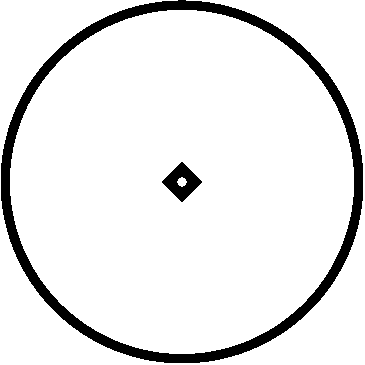
\includegraphics[width=0.155\textwidth]{symmetries/27.pdf}
      &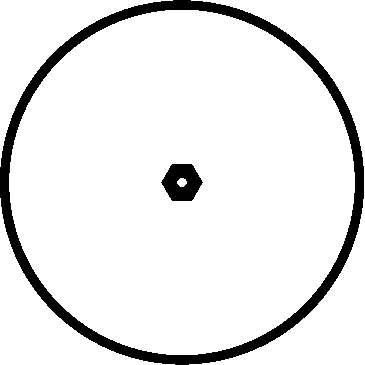
\includegraphics[width=0.155\textwidth]{symmetries/35.pdf}
      &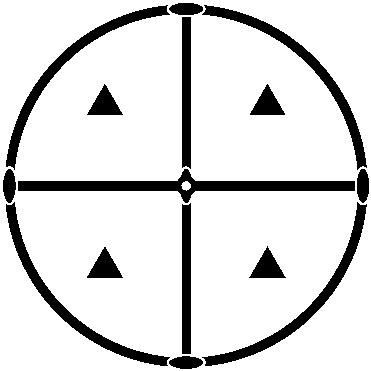
\includegraphics[width=0.155\textwidth]{symmetries/42.pdf}\\
      \multicolumn{1}{|c|}{$\overline{1}$ $(\mathrm C_{\mathrm i})$}
      & $\frac{2}{\mathrm m}$ $(\mathrm C_{2\mathrm h})$
      & $\overline{3}$ $(\mathrm C_{3\mathrm i})$
      & $\frac{4}{\mathrm m}$ $(\mathrm C_{4\mathrm h})$
      & $\frac{6}{\mathrm m}$ $(\mathrm C_{6\mathrm h})$
      & $\mathrm m\overline{3}=\frac{2}{\mathrm m}\overline{3}$ $(\mathrm T_{\mathrm h})$ \\[1ex]
      \cline{1-2} %& 1 & 1 & & &\\
      &  orthorhombic & & & &\\
      &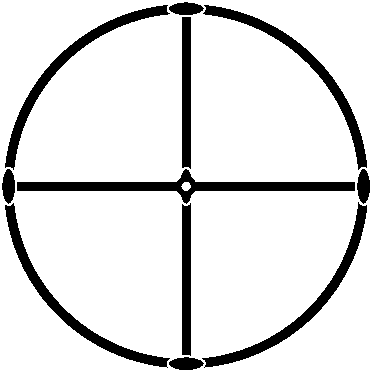
\includegraphics[width=0.155\textwidth]{symmetries/16.pdf}
      &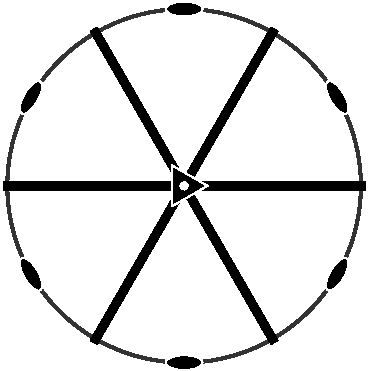
\includegraphics[width=0.155\textwidth]{symmetries/24.pdf}
      &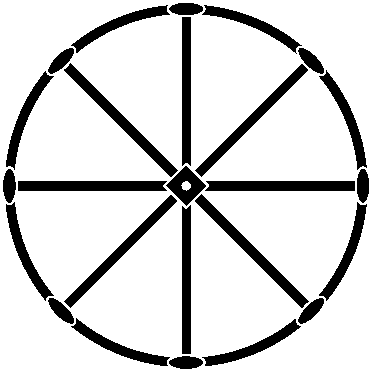
\includegraphics[width=0.155\textwidth]{symmetries/32.pdf}
      &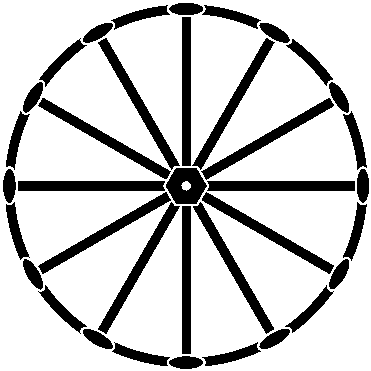
\includegraphics[width=0.155\textwidth]{symmetries/40.pdf}
      &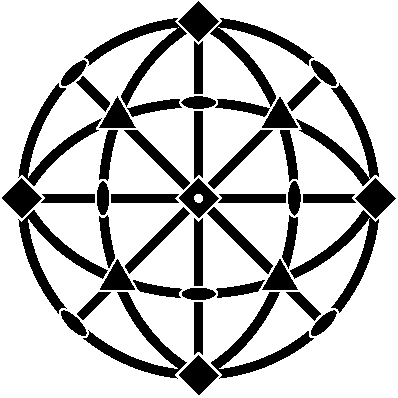
\includegraphics[width=0.155\textwidth]{symmetries/45.pdf}\\
      & mmm $(\mathrm D_{2\mathrm h})$
      & $\overline{3}\mathrm m=\overline{3}\frac{2}{\mathrm m}$ $(\mathrm D_{3\mathrm d})$
      & 4/mmm $(\mathrm D_{2\mathrm h})$
      & 6/mmm $(\mathrm D_{6\mathrm h})$
      & m$\overline{3}$m $(\mathrm O_{\mathrm h})$\\
      \cline{2-6}
    \end{tabular}
  \end{center}
\end{frame}


\begin{frame}
  \frametitle{10 mixed groups}

\begin{center}
    \setlength{\tabcolsep}{2pt}
    \begin{tabular}{cccccc}
      \hline
      \multicolumn{1}{|c}{monoclinic}
      & \multicolumn{1}{|c}{orthorhombic}
      & \multicolumn{1}{|c}{trigonal}
      & \multicolumn{1}{|c}{tetragonal}
      & \multicolumn{1}{|c}{hexagonal}
      & \multicolumn{1}{|c|}{cubic}\\
      \multicolumn{1}{|c}{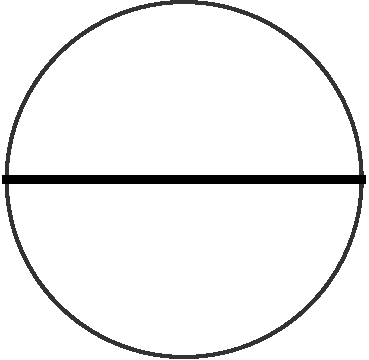
\includegraphics[width=0.155\textwidth]{symmetries/7.pdf}}
      &\multicolumn{1}{|c}{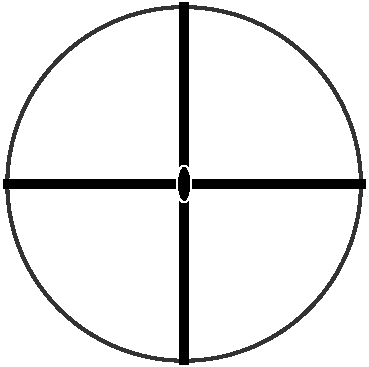
\includegraphics[width=0.155\textwidth]{symmetries/15.pdf}}
      &\multicolumn{1}{|c}{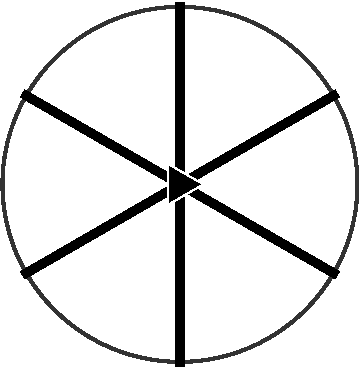
\includegraphics[width=0.155\textwidth]{symmetries/20.pdf}}
      &\multicolumn{1}{|c}{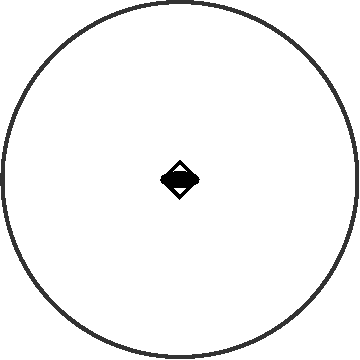
\includegraphics[width=0.155\textwidth]{symmetries/26.pdf}}
      &\multicolumn{1}{|c}{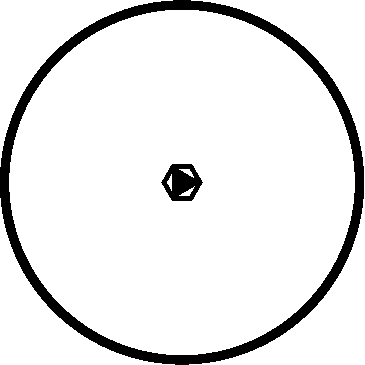
\includegraphics[width=0.155\textwidth]{symmetries/34.pdf}}
      &\multicolumn{1}{|c|}{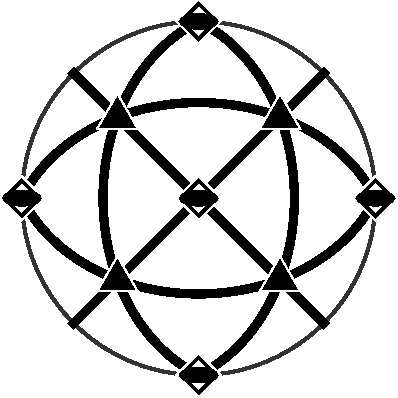
\includegraphics[width=0.155\textwidth]{symmetries/44.pdf}}\\
      \multicolumn{1}{|c}{$\overline{2}=\mathrm m$ $(\mathrm C_{\mathrm s})$}
      & \multicolumn{1}{|c}{$\mathrm m \mathrm m 2$ $(\mathrm C_{2\mathrm v})$}
      & \multicolumn{1}{|c}{$3 \mathrm m$ $(\mathrm C_{3\mathrm v})$}
      & \multicolumn{1}{|c}{$\overline{4}$ $(\mathrm S_{4})$}
      &  \multicolumn{1}{|c}{$\overline{6}$ $(\mathrm C_{3\mathrm h})$}
      &  \multicolumn{1}{|c|}{$\overline{4}3\mathrm m$ $(\mathrm
        T_{\mathrm d})$} \\[1ex]
      \cline{1-3}\cline{6-6}
      & &
      \multicolumn{1}{|c}{} & & \multicolumn{1}{|c}{} & \multicolumn{1}{c|}{}\\
      &
      & \multicolumn{1}{|c}{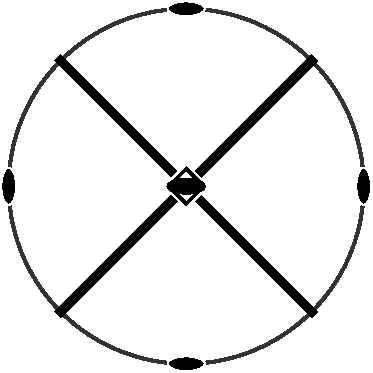
\includegraphics[width=0.155\textwidth]{symmetries/30.pdf}}
      & 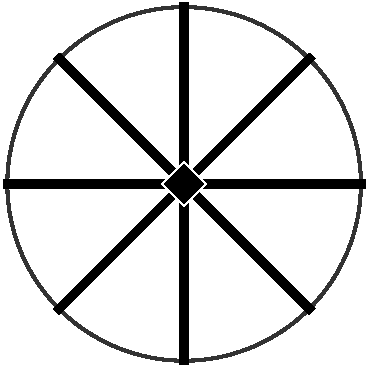
\includegraphics[width=0.155\textwidth]{symmetries/29.pdf}
      & \multicolumn{1}{|c}{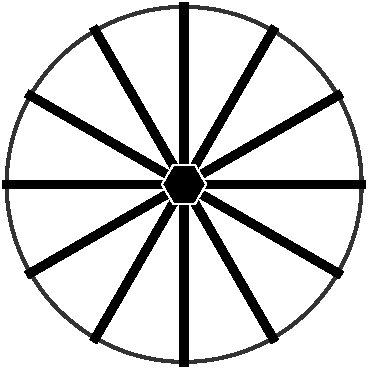
\includegraphics[width=0.155\textwidth]{symmetries/37.pdf}}
      & \multicolumn{1}{c|}{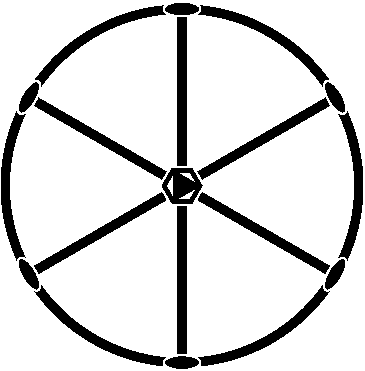
\includegraphics[width=0.155\textwidth]{symmetries/39.pdf}}\\
      &
      & \multicolumn{1}{|c}{$\overline{4}2\mathrm m$ $(\mathrm D_{2\mathrm d})$}
      & 4mm $(\mathrm C_{4\mathrm v})$
      & \multicolumn{1}{|c}{6mm $(\mathrm C_{6\mathrm v})$}
      & \multicolumn{1}{c|}{$\overline{6}$m2 $(\mathrm D_{3\mathrm h})$}\\
      \cline{3-6}
    \end{tabular}
  \end{center}

\end{frame}

% \begin{frame}
%   \frametitle{Mixed Groups}

%   \begin{tabular}{cllll}
%     & $\mat R_{\vec z,0}$ & $\alert{-}\mat R_{\vec z,90}$
%     & $\mat R_{\vec z,180}$ & $\alert{-}\mat R_{\vec z,270}$\\
%     \midrule
%     $\mat R_{\vec x,0}$
%     & $\mat R_{\vec z,0}$ & $\alert{-}\mat R_{\vec z,90}$
%     & $\mat R_{\vec z,180}$ & $\alert{-}\mat R_{\vec z,270}$\\
%     $\structure{\mathbf{-}}\mat R_{\vec x,180}$
%     & $\mat R_{\vec x,180}$ & $\alert{-}\mat R_{\vec x + \vec y,180}$
%     & $\mat R_{\vec y,180}$ & $\alert{-}\mat R_{\vec x - \vec x,180}$\\
%   \end{tabular}


% \end{frame}

% \begin{frame}
%   \frametitle{Summary Symmetry Groups}

%   \begin{itemize}
%   \item<+-> 11 purely rotational (enatiomorphic) groups:
%     %{\tikz \draw[fill=blue] (0,0) circle[radius=1.5pt];}
%     \begin{itemize}
%     \item[\mycirc] used in most software,
%     \item[\mycirc]  only proper rotations are considered
%     \end{itemize}
%   \item<+-> 11 Laue groups (with inversion center, centrosymmetric groups):
%     \begin{itemize}
%     \item[\mycirc] correct models for most diffraction experiments, e.g. X-ray diffraction, EBSD
%     \item[\mycirc] only few physical properties are not centrosysmmetric e.g., piezoelectricity
%     \end{itemize}
%   \item<+-> 10 mixed groups
%     \begin{itemize}
%     \item[\mycirc] without inversion center
%     \item[\mycirc] each with equally many proper and improper symmetry elements
%     \end{itemize}
%   \item<+-> 32 different point groups
%     \begin{itemize}
%     \item[\mycirc] do \alert{not} represent actual symmetries of the atom
%       lattice - only modulu translation
%     \end{itemize}
%   \item<+-> 230 different point groups
%       \begin{itemize}
%       \item[\mycirc] The translation vectors always coincide with the screw
%         axes.
%       \item[\mycirc] completely described in \emph{International Tables for Crystallography}, 2016
%       \end{itemize}
%   \end{itemize}

% %   \begin{itemize}
% %   \item $-\mat R_{\vec a, \pi}, -\mat R_{\vec b, \pi} \in \mathcal P$,
% %     $\angle(\vec a,\vec b) \frac{\pi}{n}$
% %     $\implies$ $\mat R_{\vec a \times \vec b, \frac{2\pi}2} \in \mathcal P$
% %   \item $-\mat R_{\vec a, \pi}, \mat R_{\vec b, \pi} \in \mathcal P$,
% %     $\angle(\vec a,\vec b) \frac{\pi}{n}$
% %     $\implies$ $-\mat R_{\vec a \times \vec b, \frac{2\pi}2} \in \mathcal P$
% % \end{itemize}

% \end{frame}


% \begin{frame}
%   \frametitle{The 230 Space Groups}

%   \begin{Theorem}
%     In a screw axis the translation vector always coincides with the
%     rotational axis.
%   \end{Theorem}
%   \begin{proof}
%     \begin{itemize}
%     \item $\mat S = (\mat R,\vec t)$
%     \item
%     \end{itemize}

%   \end{proof}

% \end{frame}

\begin{frame}[fragile]
  \frametitle{Defining Crystal Symmetries in MTEX}

\begin{lstlisting}[style=input]
cs = crystalSymmetry('m-3m')  % by international symbol
cs = crystalSymmetry('Oh')    % by Schoenflies notation
cs = crystalSymmetry('Fm-3m') % by space group

% import CIF file
cs = crystalSymmetry.load('quartz.cif')

% download from Crystallography Open Database
cs = crystalSymmetry.load('5000036')
\end{lstlisting}




\begin{lstlisting}[style=input]
cs.properGroup
cs.Laue
cs.rot
\end{lstlisting}

\begin{lstlisting}[style=input]
cs.how2plot.east = cs.bAxis  
plot(cs)
\end{lstlisting}

\end{frame}


% \begin{frame}
%   \frametitle{The 14 Bravais lattices}

%   \structure{Question:} Which lattices are compatible with the symmetry groups?

%   \bigskip

%   \begin{overlayarea}{\textwidth}{6cm}

%     %\only<1|handout:0>{\centering 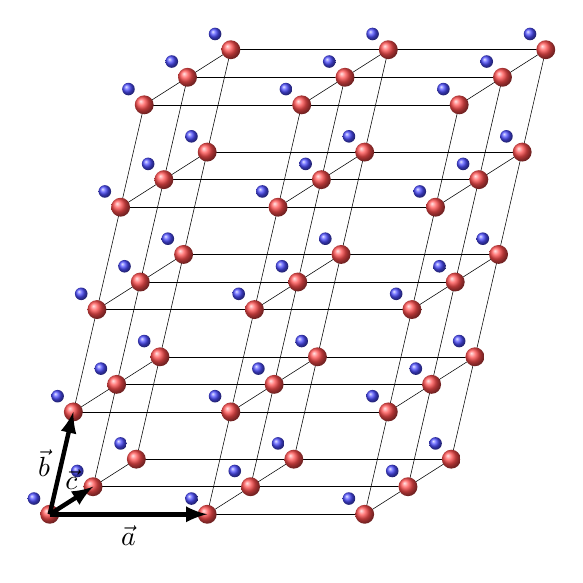
\begin{tikzpicture}[x  = {(1cm,0cm)},
  y  = {(0cm,1cm)},
  z  = {(0.35cm,0.35cm)},
  scale = 1]

  % angle
  % \filldraw[fill=red!35,draw=red!45,opacity=0.5]
  % (3,0.5) -- (1,0.5) arc (180:147:2) -- cycle;
  % \draw (1.75,0.6) node[above] {$\theta$};

  % grid
  % \draw[style=help lines,color=red!45][step=0.5cm] (-0.4,0.1) grid (6.4,2.4);
  % \draw[color=red!70, thick] (-0.4,0.5) -- (6.4,0.5);
  % \draw[->, >=latex, color=red!70, thick] (3,0.1) -- (3,3) node[left] {$\bf h$};

  \def\dax{2}
  \def\day{0.3}
  \def\daz{0.2}
  \def\dby{1.3}

  % grid
  \foreach \y in {0,1,...,4}
  \foreach \z in {0,1,...,2}
  \draw[style=help lines,color=black] (\dax*0+\day*\y+\daz*\z,\dby*\y,\z)
  -- (\dax*2+\day*\y+\daz*\z,\dby*\y,\z);

  \foreach \x in {0,1,...,2}
  \foreach \z in {0,1,...,2}
  \draw[style=help lines,color=black] (\dax*\x+\day*0+\daz*\z,\dby*0,\z)
  -- (\dax*\x+\day*4+\daz*\z,\dby*4,\z);

  \foreach \x in {0,1,...,2}
  \foreach \y in {0,1,...,4}
  \draw[style=help lines,color=black] (\dax*\x+\day*\y+\daz*0,\dby*\y,0)
  -- (\dax*\x+\day*\y+\daz*2,\dby*\y,2);

  % path to vector h
  % \draw[->, >=latex, ultra thick, color=green, style=dashed] (0,0,0) ->
  % +(\dax*3,0,0) -> +(\dax*3+\daz*1,0,1) -> (\dax*3+\day*2+\daz*1,\dby*2,1);

  % atoms
  \foreach \x in {0,1,...,2}
  \foreach \y in {0,1,...,4}
  \foreach \z in {0,1,...,2}
  {
  \shade[ball color=red!70] (\dax*\x+\day*\y+\daz*\z,\dby*\y,\z) circle (.12cm);
  \shade[ball color=blue!70] (\dax*\x+\day*\y+\daz*\z-0.2,\dby*\y+0.2,\z) circle (.08cm);
  }

  % unit cell
  \draw[->, >=latex, ultra thick] (0,0,0) -> node[left] {$\vec{b}$}
  (\day,\dby,0);
  \draw[->, >=latex, ultra thick, color=black]
  (0,0,0) -> node[below] {$\vec{a}$} (\dax,0,0);
  \draw[->, >=latex, ultra thick, color=black]
  (0,0,0) -> node[above] {$\vec{c}$} (\daz,0,1);

  % vector
  % \draw[->, >=latex, thick] (0,0,0) -> node[above] {$\vec h$}
  % (\dax*3+\day*2+\daz*1,\dby*2,1);
\end{tikzpicture}

%%% Local Variables:
%%% mode: latex
%%% TeX-master: "ChapterOne"
%%% End:
}

%     \begin{onlyenv}<2-3> Compatibility with the points groups leads to the
%       \structure{7 crystal systems:}

%       \begin{block}{}
%         \mycirc triclinic \mycirc monoclinic \mycirc orthorhombic \mycirc trigonal
%         \mycirc tetragonal \mycirc hexagonal \mycirc cubic
%       \end{block}
%     \end{onlyenv}

%     \bigskip

%     \begin{onlyenv}<3> Compatibility with the space groups leads to the
%       \structure{the 14 Bravais lattices} which additionally separates how the
%       atoms are aligned with the lattice points:
%       \begin{itemize}
%       \item \structure{primitive}
%       \item \structure{base centered}
%       \item \structure{body centered}
%       \item \structure{face centered}
%       \end{itemize}


%     \end{onlyenv}



% \end{overlayarea}


% \end{frame}

% \begin{frame}

%   \begin{table}
%     \centering

%     \begin{tabular}{>{\centering\bfseries}m{0.6in}
%       >{\centering\arraybackslash}m{1.1in}
%       >{\centering\arraybackslash}m{1.1in}
%       >{\centering\arraybackslash}m{1.1in}
%       >{\centering\arraybackslash}m{1.1in}}
%       \textbf{system}
%       & \textbf{P ({\footnotesize primitive})}
%       & \textbf{C ({\footnotesize base centered})}
%       & \textbf{I ({\footnotesize body centered})}
%       & \textbf{F ({\footnotesize face centered})}\\
%       \midrule
%       \makecell[bl]{\textbf{triclinic}\\ \footnotesize $a \ne  b \ne  c$,\\
%       \footnotesize $\alpha  \ne  \beta \ne \gamma$}
%       & 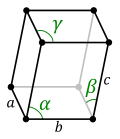
\includegraphics[height=2cm]{bravais/Triclinic.png}
%       &&\\
%       \makecell[bl]{\textbf{mononclinic}\\ \footnotesize $a \ne  b \ne  c$,\\
%       \footnotesize $\alpha  =  \gamma = 90\degree$\\
%       \footnotesize $\beta > 90 \degree$}
%       & 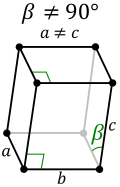
\includegraphics[height=2.5cm]{bravais/Monoclinic.png}
%       & 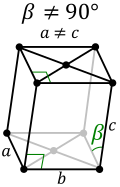
\includegraphics[height=2.5cm]{bravais/Monoclinic-base-centered.png}& \\
%       \makecell[bl]{\textbf{orthorhombic}\\ \footnotesize $a \ne  b \ne c$,\\
%       \footnotesize $\alpha  =  \beta = 90\degree$\\
%       \footnotesize $\gamma = 90\degree$}
%       & 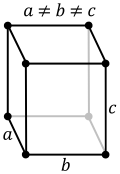
\includegraphics[height=2.3cm]{bravais/Orthorhombic.png}
%       & 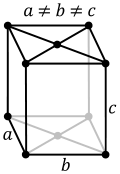
\includegraphics[height=2.3cm]{bravais/Orthorhombic-base-centered.png}
%       & 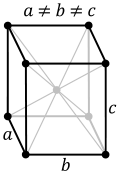
\includegraphics[height=2.3cm]{bravais/Orthorhombic-body-centered.png}
%       & 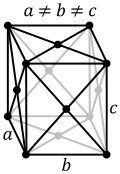
\includegraphics[height=2.3cm]{bravais/Orthorhombic-face-centered.png}
%     \end{tabular}
% \end{table}

% \end{frame}


% \begin{frame}

%   \begin{table}
%     \centering
%     \begin{tabular}{>{\centering\bfseries}m{0.6in}
%       >{\centering\arraybackslash}m{1.1in}
%       >{\centering\arraybackslash}m{1.1in}
%       >{\centering\arraybackslash}m{1.1in}
%       >{\centering\arraybackslash}m{1.1in}}
%       \textbf{system}
%       & \textbf{P ({\footnotesize primitive})}
%       & \textbf{C ({\footnotesize base centered})}
%       & \textbf{I ({\footnotesize body centered})}
%       & \textbf{F ({\footnotesize face centered})}\\
%       \midrule
%       \makecell[bl]{\textbf{tetragonal}\\ \footnotesize $a =  b \ne  c$,\\
%       \footnotesize $\alpha  =  \beta = 90\degree$\\
%       \footnotesize $\gamma = 90\degree$}
%       & 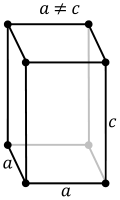
\includegraphics[height=1.7cm]{bravais/Tetragonal.png}
%       &
%       & 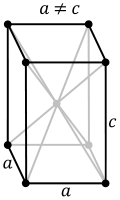
\includegraphics[height=1.7cm]{bravais/Tetragonal-body-centered.png}  \\[-2ex]
%       \makecell[bl]{\textbf{trigonal}\\ \footnotesize $a =  b \ne  c$,\\
%       \footnotesize $\alpha  =  \beta = 90\degree$\\
%       \footnotesize $\gamma = 120\degree$}
%       & 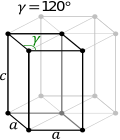
\includegraphics[height=1.7cm]{bravais/Hexagonal.png}
%       &
%       &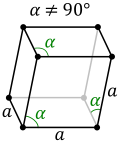
\includegraphics[height=1.7cm]{bravais/Rhombohedral.png}\\[-2ex]
%       \makecell[bl]{\textbf{hexagonal}\\ \footnotesize $a =  b \ne  c$,\\
%       \footnotesize $\alpha  =  \beta = 90\degree$\\
%       \footnotesize $\gamma = 120\degree$}
%       & 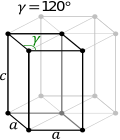
\includegraphics[height=1.7cm]{bravais/Hexagonal.png}
%       & & \\[-2ex]
%       \makecell[bl]{\textbf{cubic}\\ \footnotesize $a =  b = c$,\\
%       \footnotesize $\alpha  =  \beta = 90\degree$\\
%       \footnotesize $\gamma = 90\degree$}
%       & 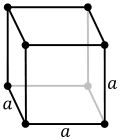
\includegraphics[height=1.7cm]{bravais/Cubic.png}
%         &
%       & 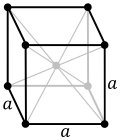
\includegraphics[height=1.7cm]{bravais/Cubic-body-centered.png}
%       & 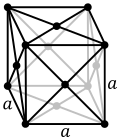
\includegraphics[height=1.7cm]{bravais/Cubic-face-centered.png}
%     \end{tabular}
% \end{table}

% \end{frame}


% \begin{frame}
%   \frametitle{A Practical Example}

%   \begin{itemize}
%   \item checkout \url{https://materialsproject.org/materials/mp-2657/\#}
%   \item download cif file
%   \end{itemize}



% \end{frame}


\begin{frame}
  \frametitle{The Ambiguity of the Crystal Coordinate System}

  \begin{overlayarea}{\textwidth}{7.5cm}
    the axes of the crystal coordinate system $\vec a$, $\vec b$, $\vec c$ are
    always chosen such that
    \begin{itemize}
    \item the translations $\mat T_{\vec a}$, $\mat T_{\vec b}$,
      $\mat T_{\vec c}$ are symmetry elements of the space group
    \item $\vec c$ is the axis of highest symmetry (except for monoclinic and
      $23$)
    \item $\vec a$ or $\vec b$ are aligned with the symmetry axes
      perpendicular to $\vec c$
    \end{itemize}

    \pause
    \medskip

    \begin{beamerboxesrounded}{critical symmetries}
      \begin{description}[orthorhombic:]
      \item[monoclinic]<+-> alignment of the two fold axis: $211$, $121$,
        $112$, $m11$, $1m1$, $11m$,
      \item[orthorhombic]<+-> alignment of the two fold axis: $2mm$, $m2m$,
        $mm2$
      \item[trigonal]<+-> alignment of the two fold axis: $321$, $312$
      \end{description}
    \end{beamerboxesrounded}

    \vspace{-0.2cm}

    \begin{onlyenv}<2>
      \begin{center}
        
\includegraphics[height=2.7cm]{symmetries/3}
        
\includegraphics[height=2.7cm]{symmetries/6}
        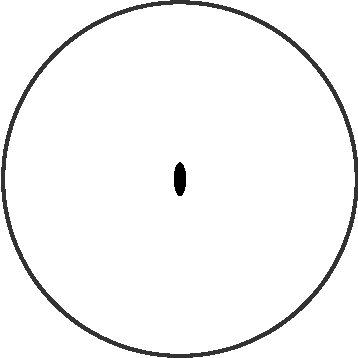
\includegraphics[height=2.7cm]{symmetries/9}
      \end{center}

    \end{onlyenv}

    \begin{onlyenv}<3|handout=0>
      \begin{center}
        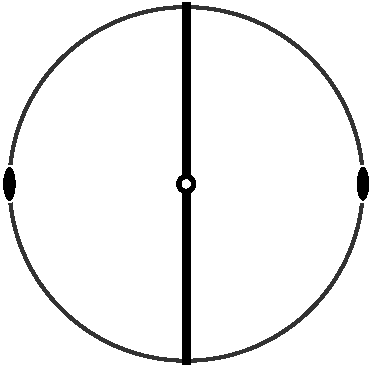
\includegraphics[height=2.7cm]{symmetries/5}
        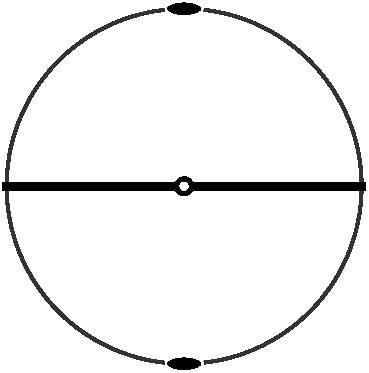
\includegraphics[height=2.7cm]{symmetries/8}
        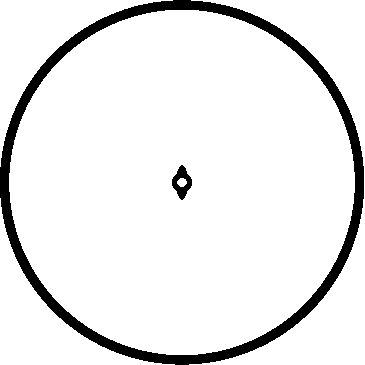
\includegraphics[height=2.7cm]{symmetries/11}
      \end{center}

    \end{onlyenv}

    \begin{onlyenv}<4|handout=0>
      \begin{center}
        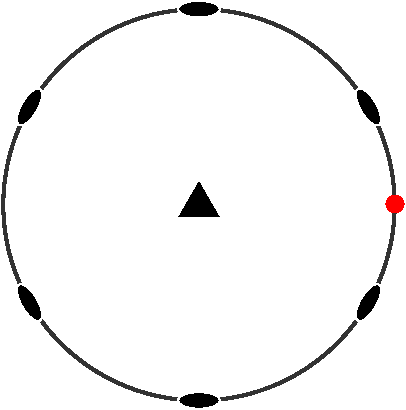
\includegraphics[height=2.7cm]{pic/sym312WithA}
        \includegraphics[height=2.7cm]{pic/sym321WithA}
        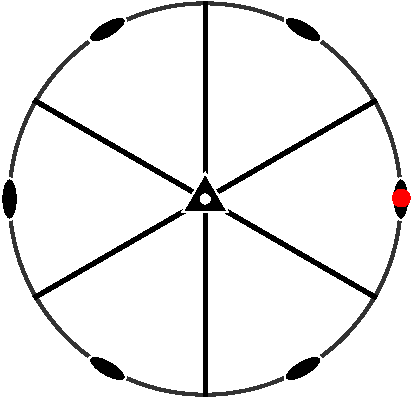
\includegraphics[height=2.7cm]{pic/sym-3m1WithA}
        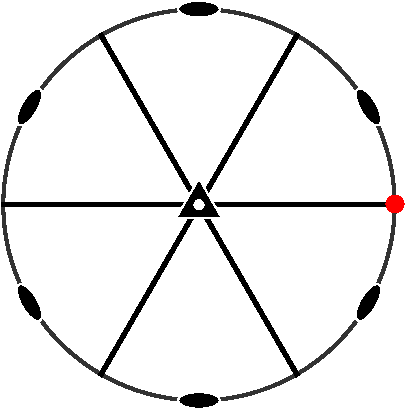
\includegraphics[height=2.7cm]{pic/sym-31mWithA}
      \end{center}
    \end{onlyenv}

  \end{overlayarea}
\end{frame}


\begin{frame}
  \frametitle{Symmetrically Equivalent Lattice Directions}

  The crystal axes $\vec a$, $\vec b$, $\vec c$ can be well defined modulo
  actions of the symmetry group $\mathcal S$.

  \begin{block}{}
    The axes $(\vec a, \vec b, \vec c)$ and $(\mat S \vec a, \mat S \vec
    b, \mat S \vec c)$ are physically indistinguishable for all $\mat S \in
    \mathcal S$
  \end{block}

  Two lattice directions
  \begin{align*}
    \vec d_{1}
    = u_{1} \vec a + v_{1} \vec b + w_{1} \vec c = [u_{1}v_{1}w_{1}]
       \text{ and }
    \vec d_{2}
    = u_{2} \vec a + v_{2} \vec b + w_{2} \vec c = [u_{2}v_{2}w_{2}]
  \end{align*}
  are called \structure{symmetrically equivalent} if there is a symmetry
  operation $\mat S \in \mathcal S$ such that
  \begin{equation*}
    \vec d_{2} = \mat S \vec d_{1}.
  \end{equation*}

    \begin{block}{}
    \begin{itemize}
    \item<+-> \structure{$\left< uvw \right>$} denotes the set of all lattice directions
      symmetrically equivalent to $\left[ uvw \right]$
    \item<+-> $\left< uvw \right>$ may contain at maximum $|\mathcal S|$
      different lattice directions
    \item<+-> rotational axes have fewer symmetrically equivalent crystal
      directions, e.g. $\left<001\right> = \left[001\right]$
    \item<+-> the quotient between the total number of symmetry elements
      $|\mathcal S|$ and the number of directions in $\left< uvw \right>$ is
      called \structure{multiplicity} of $\left< uvw \right>$
    \end{itemize}

  \end{block}

\end{frame}


\begin{frame}
  \frametitle{Symmetrically Equivalent Lattice Planes}

  For most symmetries the symmetrically equivalent directions comes as
  permutations of the Miller indices

    \begin{description}[orthorhombic:]
  \item[monoclinic:]<+-> $\left<uvw \right> = \left<\overline u v \overline w \right>$
  \item[orthorhombic:]<+-> $\left<uvw \right> = \left<\overline u v
      w \right> = \left< u \overline v w \right> = \left< u  v \overline w \right>$
  \item[tetragonal:]<+->  $\left<uvw \right> = \left<\overline v u
      w \right> = \left< \overline u \, \overline v w \right> = \left< v
      \overline u w \right>$
  \item[cubic:]<+->
    $\left< uvw \right> = \left< vwu \right> = \left< wuv \right> =
    \left< u\overline v \overline w \right> = \left< v\overline w \overline u
    \right> = \left< w\overline u \overline v \right> =$\\
    $\left< \overline uv\overline w \right> = \left< \overline vw\overline u \right> = \left< \overline wu\overline v \right>=
    \left<\overline  u\overline vw \right> = \left<\overline v\overline wu \right> = \left< \overline w\overline uv \right>$
  \end{description}

  \medskip

  \uncover<5>{ Analogously the class of symmetrically equivalent
    lattice planes $\{hk\ell\}$ is defined as the set of all lattice planes
    $(h_{2}k_{2}\ell_{2})$ such that there is a symmetry operation
    $\mat S \in \mathcal S$ with
    \begin{equation*}
      (h_{2}k_{2}\ell_{2})
      = h_{2} \vec a^{*} + k_{2} \vec b^{*} + \ell_{2} \vec c^{*}
      = \mat S(h \vec a^{*} + k \vec b^{*} + \ell \vec c^{*})
    \end{equation*}

    \begin{center}
      \begin{tabular}{lcc}
        \toprule
        reference system & single & symmetrically equivalent \\
        \midrule
        lattice point & $\cdot uvw \cdot$ & $:\!uvw\!:$ \\
        lattice direction & $[uvw]$  & $\left<uvw\right>$ \\
        lattice plane & $(hk\ell)$ & $\{hkl\}$ \\
        \bottomrule
      \end{tabular}
    \end{center}
  }
\end{frame}

\begin{frame}
  \frametitle{Miller Indices for Trigonal and Hexagonal Symmetries}

    \begin{columns}
      \begin{column}{0.5\textwidth}
        \begin{overlayarea}{\textwidth}{7.4cm}
          For trigonal and hexagonal symmetries symmetrically equivalent
          directions can \textbf{not} be determined by permuting the three digit Miller
          indies.

        \bigskip

        \begin{onlyenv}<2-> Solution: 4 digit Miller indices
          \begin{description}
          \item[$(HKIL)$] $H=h$, $K=k$, $i = -h-k$, $L=\ell$
          \item[${[}UVTW{]}$] $U = 2u-v$, $V = 2v-u$, $T=-u-v$, $W=3w$
          \end{description}
        \end{onlyenv}

        \bigskip

        \begin{onlyenv}<3-> symmetric planes:
          \begin{description}[hexagonal:]
          \item[trigonal:]<3-> $\{HKIL\} = \{KIHL\} = \{IHKL\}$
          \item[hexagonal:]<4->
            $\{HKIL\} = \{KIHL\} = \{IHKL\} = \{\overline{HKI}L\} =
            \{\overline{KIH}L\} = \{\overline{IHK}L\} $
          \end{description}
        \end{onlyenv}
  \end{overlayarea}

      \end{column}

      \begin{column}{0.5\textwidth}
        \centering
        \only<2->{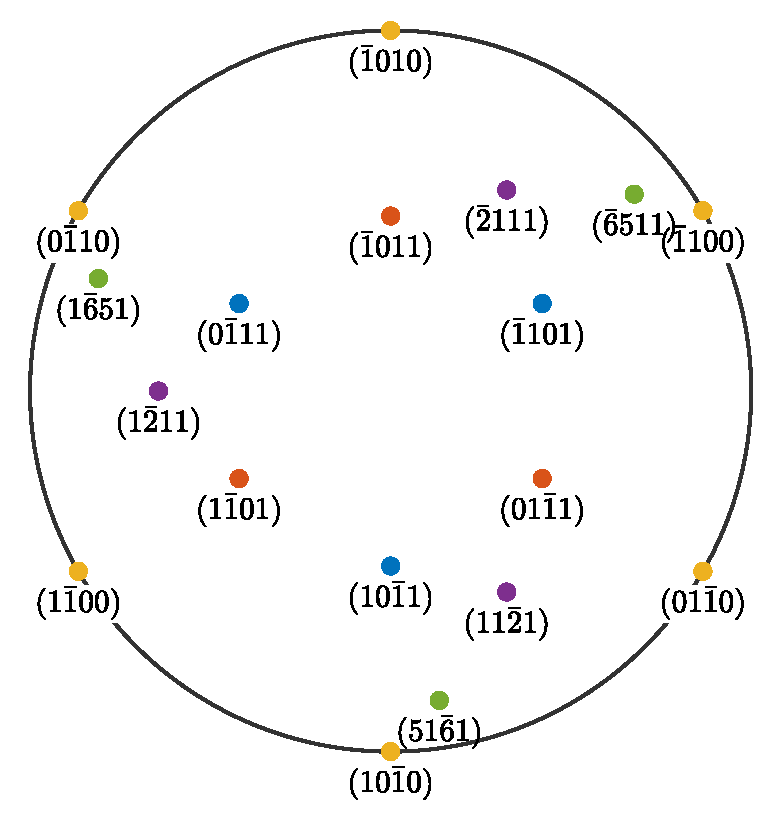
\includegraphics[width=\textwidth]{pic/quartzPlanes}}
      \end{column}
    \end{columns}


\end{frame}


\begin{frame}[fragile,fragile]
  \frametitle{MTEX}


\begin{lstlisting}[style=input]
% define some crystal direction
cs = crystalSymmetry('321',[4.9 4.9 5.4],'mineral','quartz')
h = Miller({1,0,-1,0},{0,0,0,1},cs,'UVTW')

% define some crystal plane
h = Miller({1,0,-1,0},{0,0,0,1},cs,'HKIL')

% find all symmetrically equivalent
hSym = h.symmetrise
unique(h.symmetrise,'noSymmetry')

h.multiplicity

angle(hSym(1),hSym(2))

angle(hSym(1),hSym(2),'noSymmetry')

\end{lstlisting}

\end{frame}

\begin{frame}
  \frametitle{The Fundamental Sector}

  \begin{Definition}
    The \structure{fundamental sector} is a spherical region which contains
    from each class of symmetrically equivalent vectors exactly one.
  \end{Definition}

  \begin{center}
    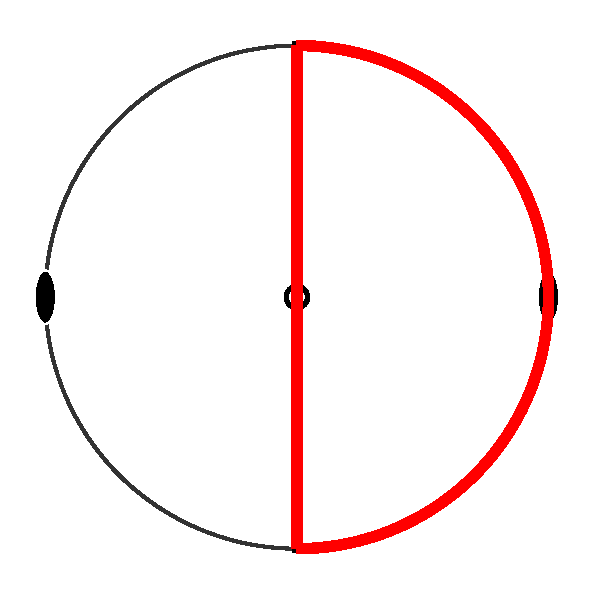
\includegraphics[scale=0.27]{pic/fundSector2_m.pdf}
    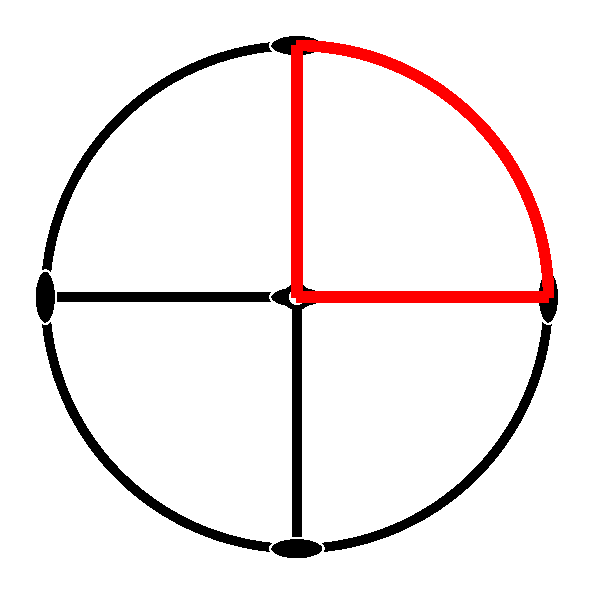
\includegraphics[scale=0.27]{pic/fundSectormmm.pdf}
    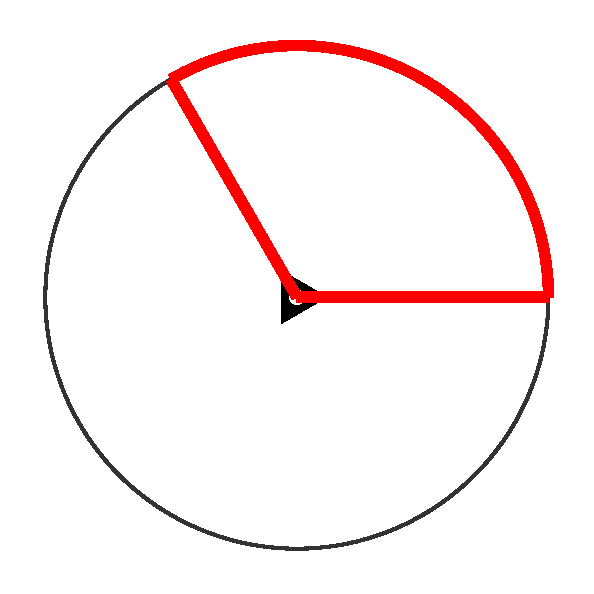
\includegraphics[scale=0.27]{pic/fundSector-3.pdf}
    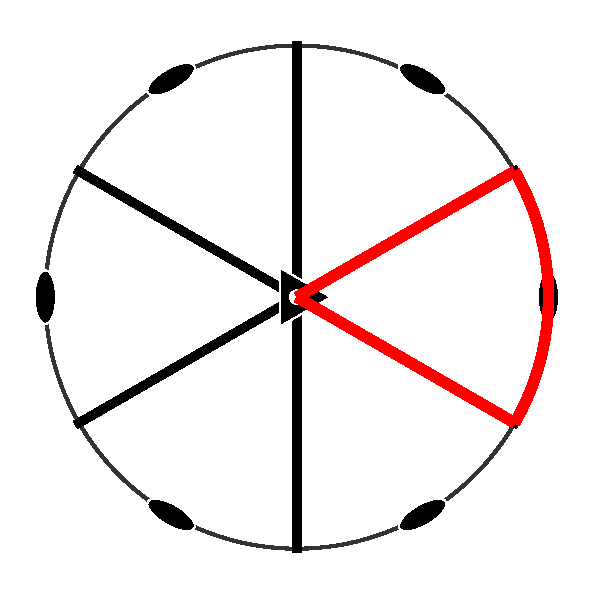
\includegraphics[scale=0.27]{pic/fundSector-3m1.pdf}
    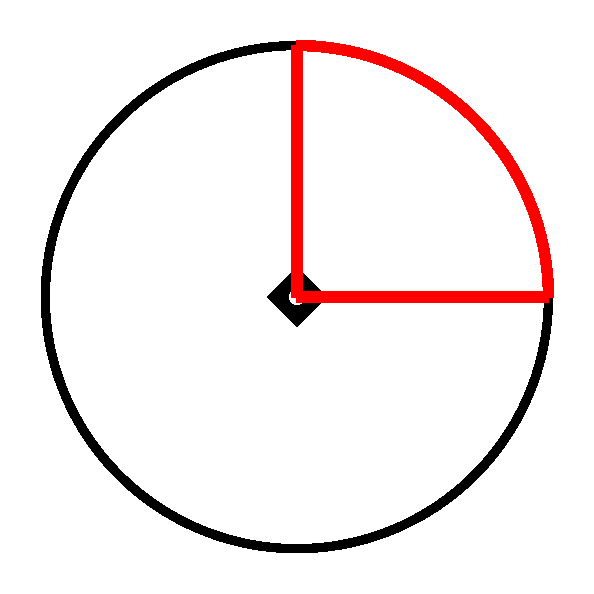
\includegraphics[scale=0.27]{pic/fundSector4_m.pdf}\\
    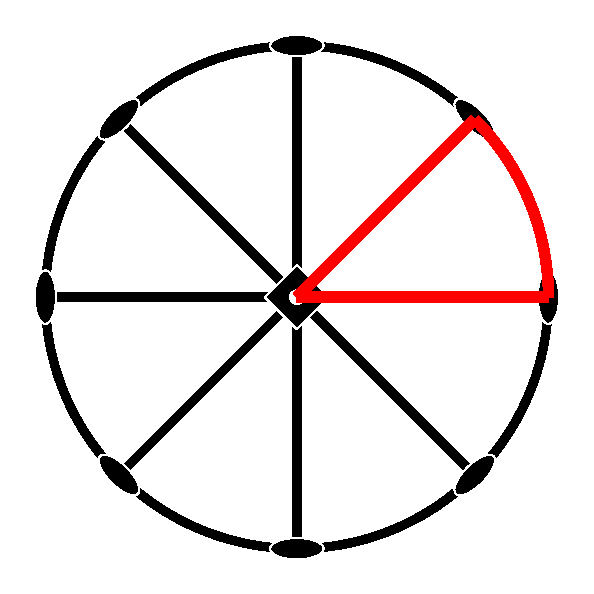
\includegraphics[scale=0.27]{pic/fundSector4_mmm.pdf}
    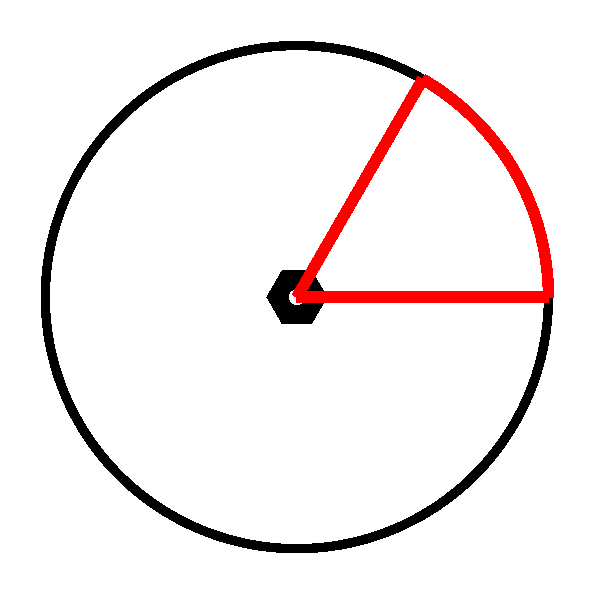
\includegraphics[scale=0.27]{pic/fundSector6_m.pdf}
    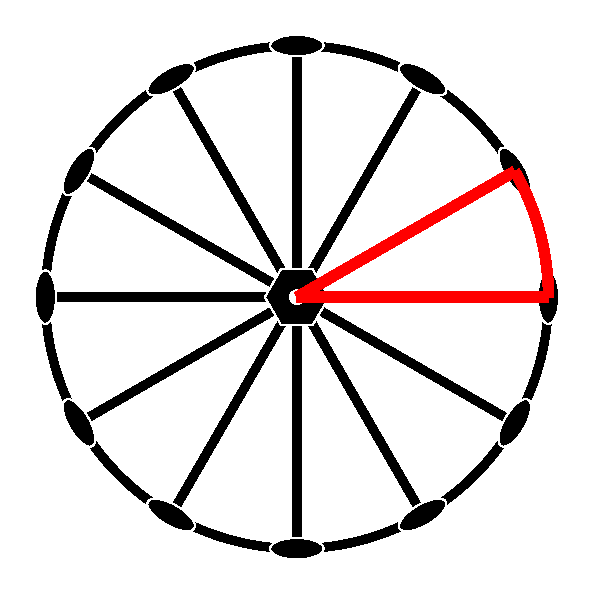
\includegraphics[scale=0.27]{pic/fundSector6_mmm.pdf}
    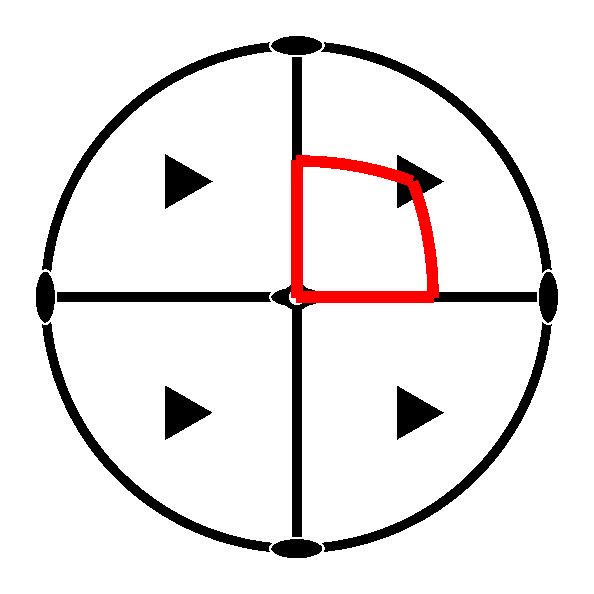
\includegraphics[scale=0.27]{pic/fundSectorm-3.pdf}
    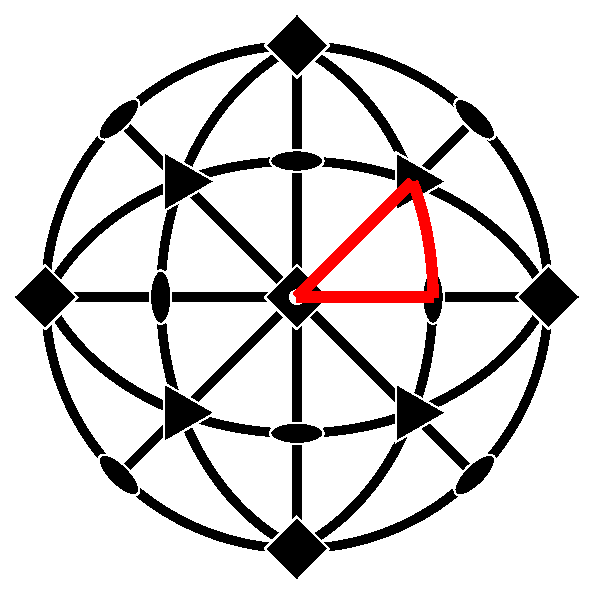
\includegraphics[scale=0.27]{pic/fundSectorm-3m.pdf}
  \end{center}

  % 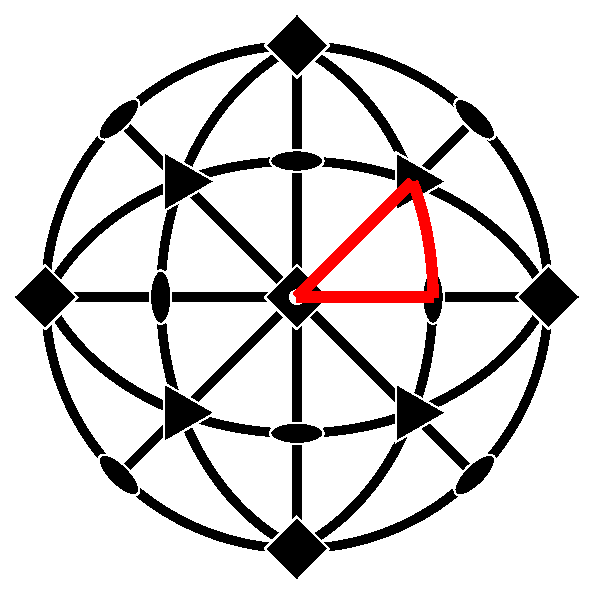
\includegraphics{pic/fundSectorm-3m.pdf}
  % 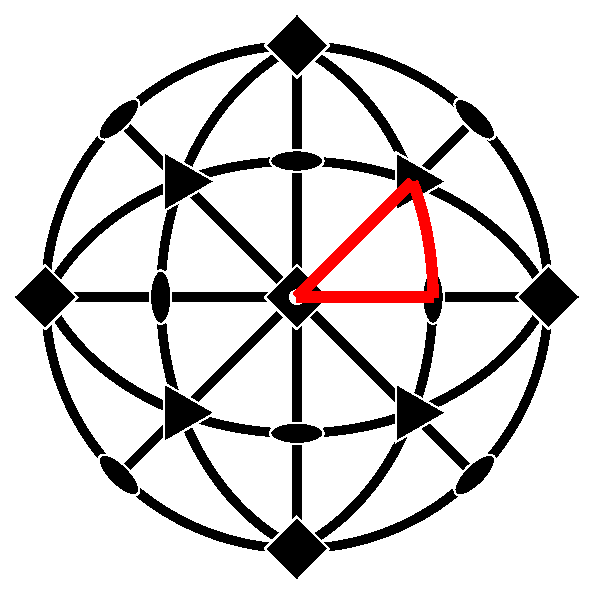
\includegraphics{pic/fundSectorm-3m.pdf}
  % 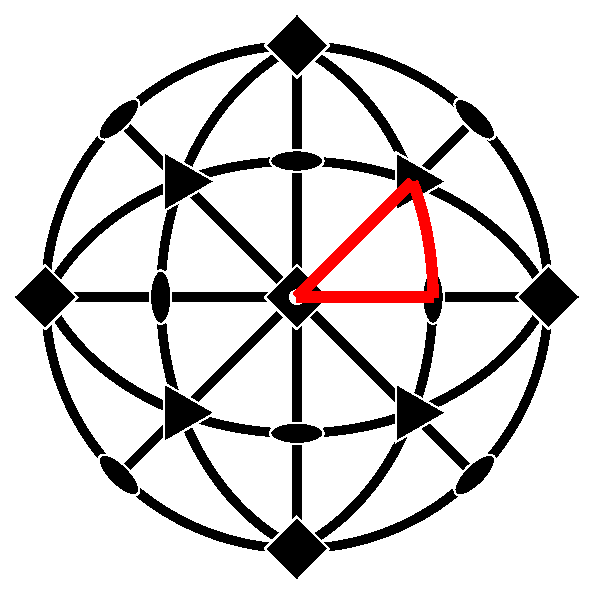
\includegraphics{pic/fundSectorm-3m.pdf}
  %   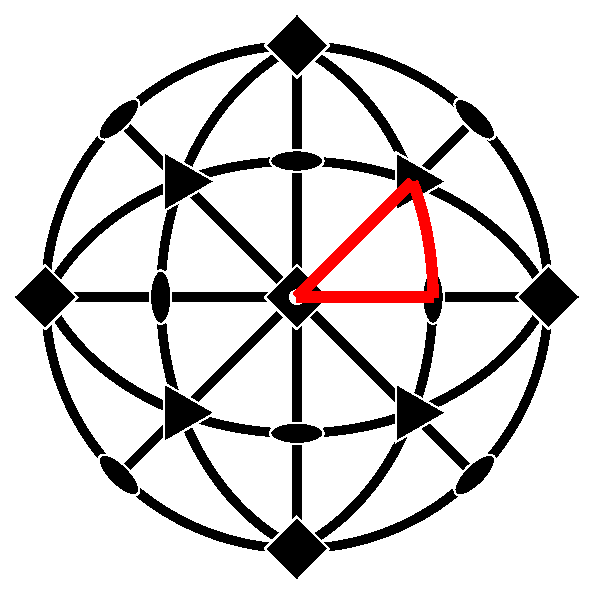
\includegraphics{pic/fundSectorm-3m.pdf}


\end{frame}

\begin{frame}[fragile,fragile]
  \frametitle{MTEX}

\begin{lstlisting}[style=input]
% the fundamental sector for a given symmetry
sR = cs.fundamentalSector
plot(sR)

% check whether we are inside the fundamental region
sR.checkInside(h)

% define some crystal plane
h = Miller({1,0,-1,0},{0,0,0,1},cs,'HKIL')
h = h.project2FundamentalRegion

% generate vectors within a spherical region
r = vector3d.rand(sR)
r = equispacedS2Grid(sR)
\end{lstlisting}

\end{frame}

% \begin{frame}
%   \frametitle{Crystals Structure}

%   \begin{center}
%     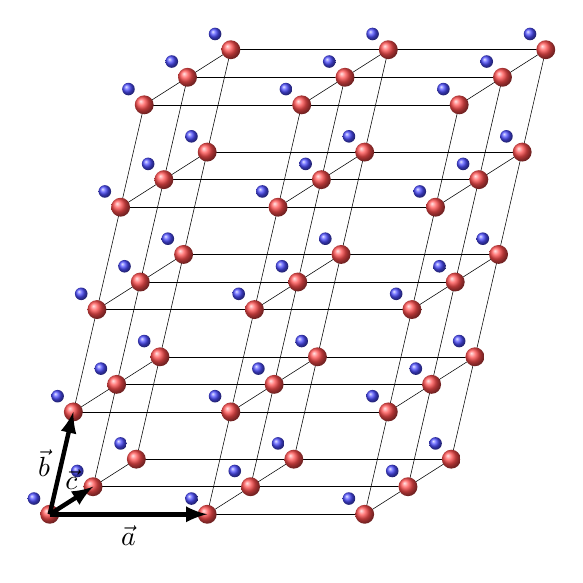
\begin{tikzpicture}[x  = {(1cm,0cm)},
  y  = {(0cm,1cm)},
  z  = {(0.35cm,0.35cm)},
  scale = 1]

  % angle
  % \filldraw[fill=red!35,draw=red!45,opacity=0.5]
  % (3,0.5) -- (1,0.5) arc (180:147:2) -- cycle;
  % \draw (1.75,0.6) node[above] {$\theta$};

  % grid
  % \draw[style=help lines,color=red!45][step=0.5cm] (-0.4,0.1) grid (6.4,2.4);
  % \draw[color=red!70, thick] (-0.4,0.5) -- (6.4,0.5);
  % \draw[->, >=latex, color=red!70, thick] (3,0.1) -- (3,3) node[left] {$\bf h$};

  \def\dax{2}
  \def\day{0.3}
  \def\daz{0.2}
  \def\dby{1.3}

  % grid
  \foreach \y in {0,1,...,4}
  \foreach \z in {0,1,...,2}
  \draw[style=help lines,color=black] (\dax*0+\day*\y+\daz*\z,\dby*\y,\z)
  -- (\dax*2+\day*\y+\daz*\z,\dby*\y,\z);

  \foreach \x in {0,1,...,2}
  \foreach \z in {0,1,...,2}
  \draw[style=help lines,color=black] (\dax*\x+\day*0+\daz*\z,\dby*0,\z)
  -- (\dax*\x+\day*4+\daz*\z,\dby*4,\z);

  \foreach \x in {0,1,...,2}
  \foreach \y in {0,1,...,4}
  \draw[style=help lines,color=black] (\dax*\x+\day*\y+\daz*0,\dby*\y,0)
  -- (\dax*\x+\day*\y+\daz*2,\dby*\y,2);

  % path to vector h
  % \draw[->, >=latex, ultra thick, color=green, style=dashed] (0,0,0) ->
  % +(\dax*3,0,0) -> +(\dax*3+\daz*1,0,1) -> (\dax*3+\day*2+\daz*1,\dby*2,1);

  % atoms
  \foreach \x in {0,1,...,2}
  \foreach \y in {0,1,...,4}
  \foreach \z in {0,1,...,2}
  {
  \shade[ball color=red!70] (\dax*\x+\day*\y+\daz*\z,\dby*\y,\z) circle (.12cm);
  \shade[ball color=blue!70] (\dax*\x+\day*\y+\daz*\z-0.2,\dby*\y+0.2,\z) circle (.08cm);
  }

  % unit cell
  \draw[->, >=latex, ultra thick] (0,0,0) -> node[left] {$\vec{b}$}
  (\day,\dby,0);
  \draw[->, >=latex, ultra thick, color=black]
  (0,0,0) -> node[below] {$\vec{a}$} (\dax,0,0);
  \draw[->, >=latex, ultra thick, color=black]
  (0,0,0) -> node[above] {$\vec{c}$} (\daz,0,1);

  % vector
  % \draw[->, >=latex, thick] (0,0,0) -> node[above] {$\vec h$}
  % (\dax*3+\day*2+\daz*1,\dby*2,1);
\end{tikzpicture}

%%% Local Variables:
%%% mode: latex
%%% TeX-master: "ChapterOne"
%%% End:

%   \end{center}

%   \begin{center}
%     crystals structure = basis + lattice
%   \end{center}

% \end{frame}


% \begin{frame}
%   \frametitle{Crystals Structure}

%   \begin{center}
%     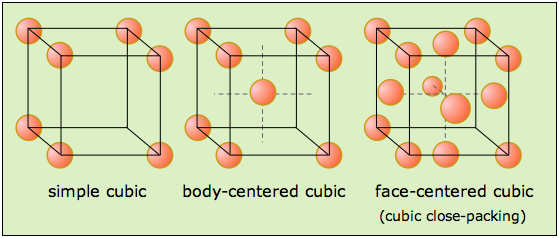
\includegraphics[width=\textwidth]{pic/fccbcc.png}
%   \end{center}

%   \begin{center}
%     crystals structure = basis + lattice
%   \end{center}

% \end{frame}


\begin{frame}
  \frametitle{Crystal Orientation}

  \begin{Definition}
    Let
    \begin{itemize}
    \item $\vec X$, $\vec Y$, $\vec Z$ - specimen fixed orthonormal coordinate
      system
    \item $\vec x$, $\vec y$, $\vec z$ - crystal fixed orthonormal coordinate
      system
    \end{itemize}
    Then the basis transformation or passive rotation $\mat O$ that translates
    crystal coordinates $(a,b,c)^{T}$ of a direction
    \begin{equation*}
      \vec v = a \vec x + b \vec y + c \vec z
    \end{equation*}
    into specimen coordinates $(A,B,C)^{T} = \mat O (a,b,c)^{T}$ satisfying
    \begin{equation*}
      \vec v = A \vec X + B \vec Y + C \vec Z
    \end{equation*}
    is called \structure{\textbf{orientation}} of the crystal lattice.

    % In matrix notation it is given explicitly as

    % \begin{equation*}
    %   \mat O =
    %   \begin{pmatrix}
    %     \text{---}\; \vec X^{t}\;\text{---}\\
    %     \text{---}\;\vec Y^{t}\;\text{---}\\
    %     \text{---}\;\vec Z^{t}\;\text{---}
    %   \end{pmatrix}
    %   \begin{pmatrix}
    %     | & | & | \\
    %     \vec x & \vec y & \vec z \\
    %     | & | & |
    %   \end{pmatrix}
    %   =
    %   \begin{pmatrix}
    %     \vec x \cdot \vec X & \vec y \cdot \vec X  & \vec z \cdot \vec X\\
    %     \vec x \cdot \vec Y & \vec y \cdot \vec Y  & \vec z \cdot \vec Y\\
    %     \vec x \cdot \vec Z & \vec y \cdot \vec Z  & \vec z \cdot \vec Z
    %   \end{pmatrix}
    % \end{equation*}

  \end{Definition}

\end{frame}

 \begin{frame}[fragile,fragile]
   \frametitle{Defining Orientations}

   by Euler angles:
      \vspace{-0.2cm}
\begin{lstlisting}[style=input]
ori = orientation.byEuler(10*degree,20*degree,30*degree,cs)
\end{lstlisting}

\medskip

by specific directions
   \vspace{-0.2cm}
\begin{lstlisting}[style=input]
n = Miller(1,1,1,'hkl',cs)
d = Miller(1,-1,0,'uvw',cs)
ori = orientation.map(n, vector3d.Z, d, vector3d.X)
\end{lstlisting}

\medskip

   by Miller indices $(hkl)[uvw]$:
   \vspace{-0.2cm}
\begin{lstlisting}[style=input]
ori = orientation.byMiller(n,d)
\end{lstlisting}

   \medskip

   by rotation matrix
   \vspace{-0.2cm}
\begin{lstlisting}[style=input]
ori = orientation.byMatrix(eye(3),cs)
\end{lstlisting}

   \medskip

   import from file
   \vspace{-0.2cm}
\begin{lstlisting}[style=input]
ori = orientation.load(fname,'Columns',{'phi1','Phi','phi2'},cs)
\end{lstlisting}


 \end{frame}


 \begin{frame}[fragile]
   \frametitle{Crystal Orientations as Coordinate Transforms}

   \begin{columns}
    \begin{column}{0.6\textwidth}
      \begin{overlayarea}{\textwidth}{0.95\textheight}
\begin{lstlisting}[style=input]
cs  = crystalSymmetry('622')
euler = [10,20,30]*degree;  
ori = orientation.byEuler(euler,cs)
h   = Miller(1,1,-2,0,cs)
\end{lstlisting}
        \vspace{-0.3cm}
        \begin{onlyenv}<1|handout:0>
\begin{lstlisting}[style=output]
ori = /+orientation+/ (/+622+/ -> xyz)

  Bunge Euler angles in degree
  phi1  Phi phi2 Inv.
    10   20   30    0

h = /+Miller+/ (/+622+/)
  h  k  i  l
  1  1 -2  0
\end{lstlisting}
        \end{onlyenv}
        \begin{onlyenv}<2->
\begin{lstlisting}[style=input]
ori * h
\end{lstlisting}
        \end{onlyenv}
        \vspace{-0.3cm}
        \begin{onlyenv}<2|handout:0>
\begin{lstlisting}[style=output]
ans = /+vector3d+/
         x        y        z
  0.702179  1.77652 0.592396
\end{lstlisting}
        \end{onlyenv}
        \begin{onlyenv}<3|handout:0>
\begin{lstlisting}[style=input]
inv(ori)
\end{lstlisting}
          \vspace{-0.3cm}
\begin{lstlisting}[style=output]
ans = /+orientation+/ (xyz -> /+622+/)

  Bunge Euler angles in degree
  phi1  Phi phi2 Inv.
   150   20  170    0
\end{lstlisting}
        \end{onlyenv}

        \begin{onlyenv}<4->
\begin{lstlisting}[style=input]
inv(ori) * vector3d.Z
\end{lstlisting}
        \end{onlyenv}
        \vspace{-0.3cm}
        \begin{onlyenv}<4|handout:0>
          \begin{lstlisting}[style=output]
ans = /+Miller+/ (/+622+/)
  h      k       i      l
  0 0.2962 -0.2962 0.9397
\end{lstlisting}
        \end{onlyenv}
        \begin{onlyenv}<5->
\begin{lstlisting}[style=input]
round(inv(ori) * vector3d.Z)
\end{lstlisting}
        \end{onlyenv}
        \begin{onlyenv}<5|handout:0>
          \vspace{-0.3cm}
\begin{lstlisting}[style=output]
ans = /+Miller+/ (/+622+/)
  h  k  i  l
  0  3 -3 10
\end{lstlisting}
        \end{onlyenv}

        \begin{onlyenv}<6->
          \begin{alertblock}{}
            Multiplication with an \texttt{\underline{orientation}} transforms an object from
            crystal into specimen coordinates. Multiplication with the inverse
            transforms it back.
          \end{alertblock}

          \begin{itemize}
          \item \texttt{vector3d, Miller}
          \item \texttt{slipSystem, dislocationSystem}
          \item \texttt{tensor}
          \end{itemize}

        \end{onlyenv}

      \end{overlayarea}
    \end{column}
    \begin{column}{0.35\textwidth}

    \end{column}
  \end{columns}
 \end{frame}




 \begin{frame}
   %\frametitle{MTEX vs. Bunge Orientation Convention}

   \begin{table}
     \centering
     \renewcommand{\arraystretch}{1.8}

     \begin{tabular}{>{\textbf}m{2.5cm}>{\centering}m{0.4\textwidth}
       >{\centering\arraybackslash}m{0.4\textwidth}}
       & \textbf{MTEX Orientations}
       & \textbf{Bunge Orientations} \\
       \midrule
       orientation
       & crystal to specimen coordinates
       & specimen to crystal coordinates\\
       Euler angles &
       $\textcolor{darkgreen}{(\varphi_{1},\Phi,\varphi_{2})}
      = \mathbf R_{\vec Z,\varphi_{1}} \mathbf R_{\vec X,\Phi}  \mathbf
       R_{\vec Z,\varphi_{2}}$
       & $\textcolor{darkgreen}{(\varphi_{1},\Phi,\varphi_{2})}
      = \mathbf R_{\vec Z'',\varphi_{2}} \mathbf R_{\vec X',\Phi}  \mathbf
         R_{\vec Z,\varphi_{1}}$\\
       Miller indices & \checked & \checked \\
       matrix
       & $\mathbf{M}^{-1}$
       & $\mathbf{M}$\\
       misorientation
       & $\mathtt{ori}_{1}^{-1} * \mathtt{ori}_{2}$
       & $\mathtt{ori}_{1} * \mathtt{ori}_{2}^{-1}$ \\
       pole figure & \checked & \checked \\
       ODF section & \checked & \checked \\
       Import & \checked & \checked \\
    \end{tabular}
\end{table}

 \end{frame}


\begin{frame}
  \frametitle{An Orthogonal Reference System}

  \begin{overlayarea}{\textwidth}{7cm}
  We will describe the orientation of a crystal lattice within a specimen by
  a basis transformation from a crystal fixed coordinate system to a specimen
  fixed coordinate system.

  \bigskip
  \pause

  \begin{columns}
    \begin{column}{0.6\textwidth}
      What do we have so far:
      \begin{itemize}
      \item<+-> a direct crystal  coordinate system $\vec a, \vec b, \vec c$
      \item<+-> a reciprocal coordinate system $\vec a^{*}, \vec b^{*}, \vec c^{*}$
      \end{itemize}

      \medskip

      \begin{block}<4->{}
        In order that the basis transformation is an orthogonal matrix we
         need  an orthogonal coordinate system $(\vec x, \vec y,
        \vec z)$ fixed to the crystal lattice.
      \end{block}

      \medskip

      \begin{uncoverenv}<4->
        There are different conventions:
        \begin{itemize}
        \item<+-> $\vec x || \vec a$, $\vec z || \vec c^{*}$
          \only<5->{\paraitem $\vec y || \vec b$, $\vec z || \vec c^{*}$}
          \only<6->{\paraitem $\vec x || \vec a^{*}$, $\vec z || \vec c$}
        \end{itemize}
      \end{uncoverenv}

  \end{column}

    \begin{column}{0.35\textwidth}
      \begin{tikzpicture}[x  = {(-0.5cm,-0.5cm)},
        y  = {(0.9659cm,-0.25882cm)},
        z  = {(0cm,1cm)},
        scale = 2]

\draw[draw=green, dashed] (0,0,0) -- (1.2,0,0) -- (1,1,0) -- (-0.2,1,0) --
(0,1.2,1) -- (0.2,0.2,1) --  (1.4,0.2,1) -- (1.2,0,0);

\draw[draw=green, dashed] (0,1.2,1) -- (1.2,1.2,1) -- (1,1,0);
\draw[draw=green, dashed] (1.2,1.2,1) -- (1.4,0.2,1);


\draw[draw=green,very thick] (0,0,0) -- (1.2,0,0) node [anchor=north,color=green!70!black] {$\vec a$};
\draw[draw=green,very thick] (0,0,0) -- (-0.2,1,0) node [anchor=west,color=green!70!black] {$\vec b$};
\draw[draw=green,very thick] (0,0,0) -- (0.2,0.2,1) node[anchor=south,color=green!70!black] {$\vec c$};

\only<1-2>{
\draw[draw=green] (0.3,0,0) arc (250:329:0.3cm);% node {$\alpha$};
\draw[draw=green] (-0.03,0.2,0) arc (0:68:0.3cm);% node {$\alpha$};
\draw[draw=green] (0.3,0,0) arc (200:112:0.3cm);% node {$\alpha$};
\node at (0.15,0.01,0.1)[color=green!70!black]{$\beta$};
\node at (0.01,0.15,0.1)[color=green!70!black]{$\alpha$};
\node at (0.15,0.1,0)[color=green!70!black]{$\gamma$};
}


\only<3->{
\draw[->,draw=red,very thick] (0,0,0) -- (0,0,1.2) node [anchor=west,color=red!70!black] {$\vec c^{*}$};
\draw[->,draw=red,very thick] (0,0,0) -- (1,0.2,-0.24) node [anchor=west,color=red!70!black] {$\vec a^{*}$};
\draw[->,draw=red,very thick] (0,0,0) -- (0,1.2,-0.24) node [anchor=north,color=red!70!black] {$\vec b^{*}$};
}

\only<4|handout>{
\draw[->,draw=black,ultra thick] (0,0,0) -- (1,0,0) node
[anchor=north,color=black] {$\vec{\mathbf x}$};
\draw[->,draw=black,ultra thick] (0,0,0) -- (0,1,0) node
[anchor=north,color=black] {$\vec{\mathbf y}$};
\draw[->,draw=black,ultra thick] (0,0,0) -- (0,0,1) node
[anchor=east,color=black] {$\vec{\mathbf z}$};
}

\only<5|handout=0>{
\draw[->,draw=black,ultra thick] (0,0,0) -- (1,0.2,0) node
[anchor=north,color=black] {$\vec{\mathbf x}$};
\draw[->,draw=black,ultra thick] (0,0,0) -- (-0.2,1,0) node
[anchor=north,color=black] {$\vec{\mathbf y}$};
\draw[->,draw=black,ultra thick] (0,0,0) -- (0,0,1) node
[anchor=east,color=black] {$\vec{\mathbf z}$};
}

\only<6-7|handout=0>{
\draw[->,draw=black,ultra thick] (0,0,0) -- (0.8,0.16,-0.192) node
[anchor=north,color=black] {$\vec{\mathbf x}$};
\draw[->,draw=black,ultra thick] (0,0,0) -- (-0.16,0.8,0.192) node
[anchor=north,color=black] {$\vec{\mathbf y}$};
\draw[->,draw=black,ultra thick] (0,0,0) -- (0.16,0.16,0.8) node
[anchor=east,color=black] {$\vec{\mathbf z}$};
}

\end{tikzpicture}

\end{column}
\end{columns}

\medskip

\begin{onlyenv}<7> \alert{The used conventions effects orientations and
    tensorial properties and should always be reported!}
\end{onlyenv}


\end{overlayarea}

\end{frame}


\begin{frame}[fragile,fragile]
  \frametitle{Defining the Orthogonal Reference Frame in MTEX}

  \begin{columns}
    \begin{column}{0.6\textwidth}
      \begin{overlayarea}{\textwidth}{0.95\textheight}
\begin{lstlisting}[style=input]
cs1 = crystalSymmetry('622')
\end{lstlisting}
        \vspace{-0.3cm}
        \begin{onlyenv}<1|handout:0>
\begin{lstlisting}[style=output]
cs1 = /+crystalSymmetry+/
  symmetry       : 622
  elements       : 12
  a, b, c        : 1, 1, 1
  reference frame: X||a*, Y||b, Z||c*
\end{lstlisting}
        \end{onlyenv}
        \begin{onlyenv}<2->
\begin{lstlisting}[style=input]
ori = orientation.rand(cs1)
\end{lstlisting}
        \end{onlyenv}
        \vspace{-0.3cm}
        \begin{onlyenv}<2|handout:0>
\begin{lstlisting}[style=output]
ori = /+orientation+/ (/+622+/ -> xyz)
  crystal symmetry : 622, X||a*, Y||b, Z||c*

  Bunge Euler angles in degree
     phi1     Phi    phi2    Inv.
  131.348 74.3274 347.732       0
\end{lstlisting}
        \end{onlyenv}
        \begin{onlyenv}<3->
\begin{lstlisting}[style=input]
cs2 = crystalSymmetry('622','x||a')
ori.CS = cs2
\end{lstlisting}
        \end{onlyenv}
        \vspace{-0.3cm}
        \begin{onlyenv}<3|handout:0>
          \begin{lstlisting}[style=output]
ori = /+orientation+/ (/+622+/ -> xyz)
  crystal symmetry : 622, X||a, Y||b*, Z||c

  Bunge Euler angles in degree
     phi1     Phi    phi2    Inv.
  131.348 74.3274 347.732       0
\end{lstlisting}
        \end{onlyenv}
        \begin{onlyenv}<4->
\begin{lstlisting}[style=input]
ori2 = ori.transformReferenceFrame(cs2)
\end{lstlisting}
        \end{onlyenv}
        \begin{onlyenv}<4|handout:0>
          \vspace{-0.3cm}
\begin{lstlisting}[style=output]
ori = /+orientation+/ (/+622+/ -> xyz)
  crystal symmetry : 622, X||a, Y||b*, Z||c

  Bunge Euler angles in degree
     phi1     Phi    phi2    Inv.
  131.348 74.3274 317.732       0
\end{lstlisting}
        \end{onlyenv}

        \medskip

        \begin{onlyenv}<5->
          the command \texttt{transformReferenceFrame}
          \begin{itemize}
          \item is available for objects of type \texttt{Miller, tensor,
              slipSystem, dislocationSystem, ODF}
          \item does not change orientation
          \item is automatically called if an operation incorporates different
            setups
        \end{itemize}
        \end{onlyenv}

      \end{overlayarea}
    \end{column}
    \begin{column}{0.25\textwidth}
      \begin{overlayarea}{\textwidth}{0.95\textheight}
        \begin{onlyenv}<1->
          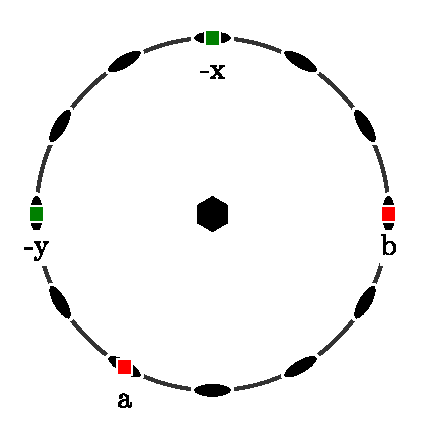
\includegraphics[width=\textwidth]{pic/622xastar}
        \end{onlyenv}
        \begin{onlyenv}<3->
          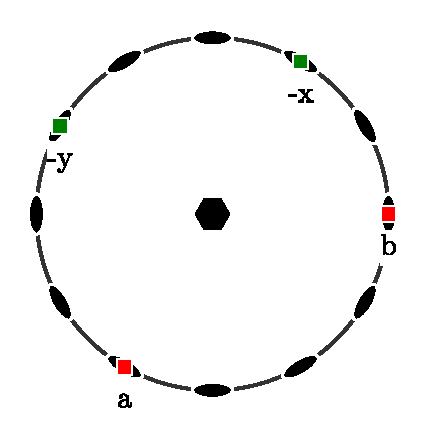
\includegraphics[width=\textwidth]{pic/622xa}
        \end{onlyenv}
      \end{overlayarea}

    \end{column}
  \end{columns}
\end{frame}






\begin{frame}[fragile]
  \frametitle{Symmetrically Equivalent Orientations}

  \begin{columns}
    \begin{column}{0.5\textwidth}
      \begin{overlayarea}{\textwidth}{0.95\textheight}
        \begin{block}{}
          Two orientations $\mat O_{1}$, $\mat O_{2}$ are
          \structure{symmetrically equivalent} if there is a symmetry
           $\mat S \in \mathcal S$ with
          \begin{equation*}
            \mat O_{2} = \mat O_{1} \mat S.
          \end{equation*}
        \end{block}

        \begin{itemize}
        \item<2-> We may either symmetrise crystal directions or orientations.
        \item<3-> The misorientation angle between symmetrically equivalent
          orientations is $0$.
        \item<4-> The crystallographic equivalent orientations form a regular
          body in $\R^{4}$.
        \item<5-> We may restrict the class of symmetrically equivalent
          orientations to a unique representative.
        \end{itemize}
      \end{overlayarea}

    \end{column}
    \begin{column}{0.45\textwidth}
      \vspace{-0.5cm}
      \begin{overlayarea}{\textwidth}{0.95\textheight}
        \begin{onlyenv}<1->
\begin{lstlisting}[style=input]
ori.symmetrise
\end{lstlisting}
        \end{onlyenv}
        \vspace{-0.3cm}
        \begin{onlyenv}<1|handout:0>
\begin{lstlisting}[style=output]
ans = /+orientation+/ (/+622+/ -> xyz)
  size: 12 x 1

  Bunge Euler angles in degree
  phi1  Phi phi2 Inv.
    10   20   30    0
   190  160  210    0
    10   20   90    0
   190  160  270    0
    10   20  150    0
   190  160  330    0
    10   20  210    0
   190  160   30    0
    10   20  270    0
   190  160   90    0
    10   20  330    0
   190  160  150    0
\end{lstlisting}
        \end{onlyenv}
        \begin{onlyenv}<2->
\begin{lstlisting}[style=input]
ori.symmetrise * h
ori * h.symmetrise
ori * cs * h
\end{lstlisting}
        \end{onlyenv}
        \vspace{-0.3cm}
        \begin{onlyenv}<2|handout:0>
\begin{lstlisting}[style=output]
ans = /+vector3d+/
 size: 12 x 1
         x        y       z
   0.89058  0.70798  0.1974
   0.89058  0.70798  0.1974
  -0.18849   1.0688  0.3949
    1.0792 -0.36061 -0.1974
   -1.0792  0.36061  0.1974
   0.18849  -1.0688 -0.3949
  -0.89058 -0.70798 -0.1974
  -0.89058 -0.70798 -0.1974
   0.18849  -1.0688 -0.3949
   -1.0792  0.36061  0.1974
    1.0792 -0.36061 -0.1974
  -0.18849   1.0688  0.3949
\end{lstlisting}
        \end{onlyenv}
        \begin{onlyenv}<3->
\begin{lstlisting}[style=input]
angle(ori, ori * cs)
\end{lstlisting}
        \end{onlyenv}
        \vspace{-0.3cm}
        \begin{onlyenv}<3|handout:0>
\begin{lstlisting}[style=output]
ans =
  0
  0
  0
  0
  0
  0
  0
  0
  0
  0
  0
  0
\end{lstlisting}
        \end{onlyenv}
        \begin{onlyenv}<4->
\begin{lstlisting}[style=input]
angle(ori, ori * cs,...
  'noSymmetry')./degree
\end{lstlisting}
        \end{onlyenv}
        \vspace{-0.3cm}
        \begin{onlyenv}<4|handout:0>
\begin{lstlisting}[style=output]
ans =
    0.0000
  180.0000
   60.0000
  180.0000
  120.0000
  180.0000
  180.0000
  180.0000
  120.0000
  180.0000
   60.0000
  180.0000
\end{lstlisting}
        \end{onlyenv}
        \begin{onlyenv}<5->
\begin{lstlisting}[style=input]
ori.project2FundamentalRegion
\end{lstlisting}
\begin{lstlisting}[style=output]
ans = /+orientation+/ (/+622+/ -> xyz)

  Bunge Euler angles in degree
  phi1  Phi phi2 Inv.
    10   20  330    0
\end{lstlisting}
        \end{onlyenv}
      \end{overlayarea}
    \end{column}
  \end{columns}

\end{frame}


\begin{frame}
  \frametitle{Fundamental Regions of the Orientation Space}

  \begin{Definition}
    The \structure{fundamental region} is a region in the space of all
    rotations which contains from each class of symmetrically equivalent
    rotations exactly one.
  \end{Definition}

  \begin{itemize}
  \item The fundamental region is no uniquely defined.
  \item Its volume is always $\frac{1}{|\mathcal S|}$ of the entire rotation
    space.
  \end{itemize}



  \begin{exampleblock}{The fundermental region in Euler angle space}
    \centering
    \begin{tabular}{lccccccccccc}
      symmetry
      & $1$ & $112$ & $222$ & $3$ & $321$ & $4$ & $422$ & $6$ & $622$ & $23$ & $432$ \\
      \midrule
      $\varphi_{1}$ & $360$ & $360$ &$360$ &$360$ &$360$ &$360$ &$360$ &$360$ &$360$ &\tikzmark{left}{$360$} & $360$\\
      $\Phi$ & $180$ & $180$ & $90$ &  $180$& $90$ & $180$& $90$ & $180$& $90$ & $90$& $90$ \\
      $\varphi_{2}$ & $360$ & $180$ & $180$ & $120$ & $120$ & $90$ &  $90$ &$60$& $60$ & $180$ & \tikzmark{right}{$90$}
    \end{tabular}
    \Highlight[first]

    \medskip

    \alert{In cubic symmetry the three fold axis is not respected.}
  \end{exampleblock}


\end{frame}



\begin{frame}
  \frametitle{Fundamental Regions as Voronoi Cells}

  We may use the rotational angle $\omega(\mat O,\tilde{\mat O})$ to define
  Voronoi cells in orientation space.

  \begin{Definition}
    Let $\mat O$ be an arbitrary orientation with symmetry group $\mathcal
    S$. The Voronoi cell $\mathcal V_{\mat O}$ is defined as all orientations
    $\tilde{\mat O}$ which have smaller distance to $\mat O$ then to any of
    its symmetrically equivalent orientations $\mat O \mat S$, $\mat S \in
    \mathcal S$, i.e.,
    \begin{equation*}
      \mathcal V_{\mat O}
      = \left\{ \tilde{\mat O} \text{ such that for all $\mat S \in \mathcal S$ }
        \omega(\tilde{\mat O},\mat O)
        \le  \omega(\tilde{\mat O},\mat O \mat S) \right\}
    \end{equation*}
  \end{Definition}

  \begin{Theorem}
    The Voronoi cell $\mathcal V_{\mat O}$ is a fundamental region which is
    bounded by the midplanes between $\mat O$ and all its symmetrically
    equivalent orientations $\mat O \mat S$, $\mat S \in \mathcal S$.
  \end{Theorem}
  % \begin{proof}

  % \end{proof}


\end{frame}

\begin{frame}
  \frametitle{Fundamental Regions in Rodrigues Space}

  Since in Rodrigues Frank space the midplanes between two orientations are
  ``real'' Euclidean planes the bounded Voronoi cells are regular polyhedrons.


  \begin{center}
    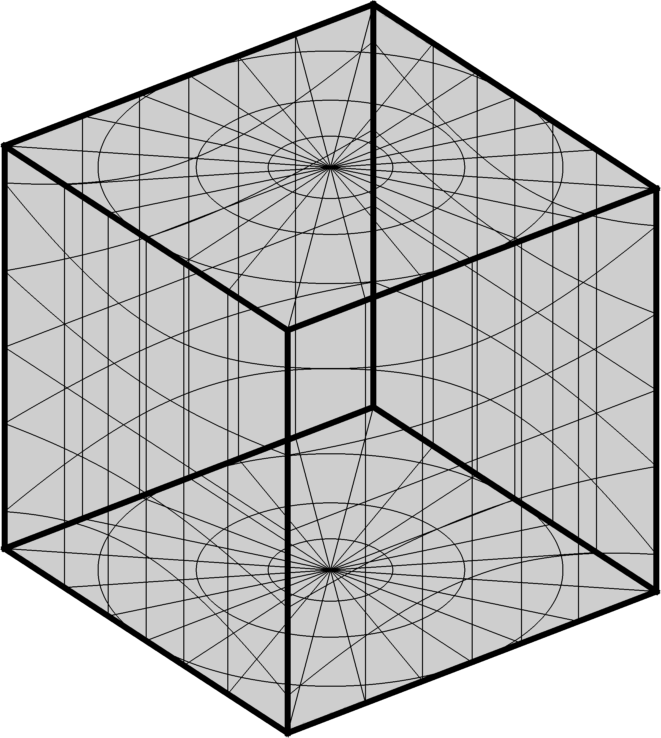
\includegraphics[width=2.8cm]{oR/Rod222} \qquad
    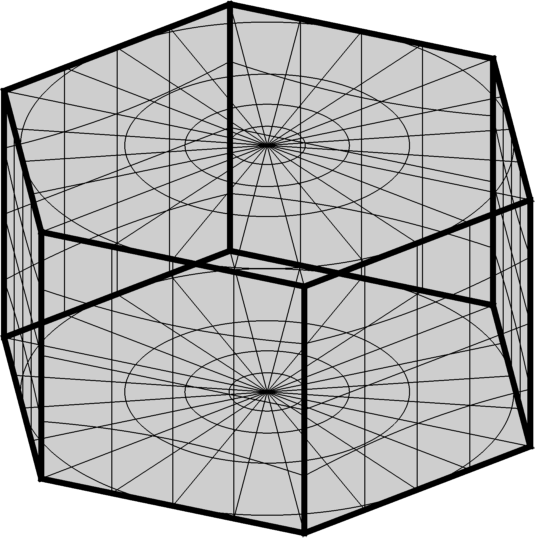
\includegraphics[width=2.8cm]{oR/Rod321} \qquad
    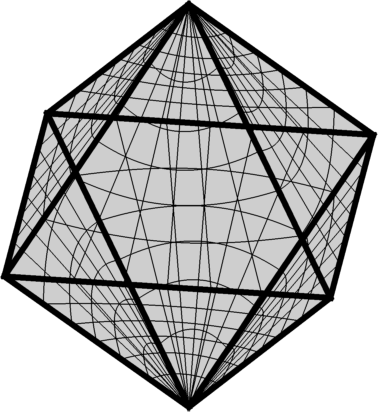
\includegraphics[width=2.8cm]{oR/Rod23} \\
    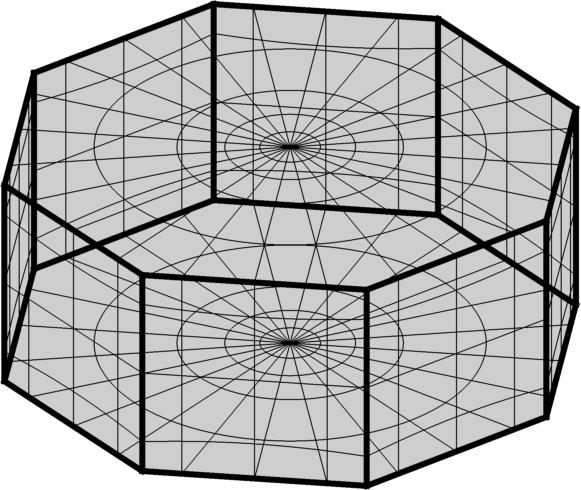
\includegraphics[width=2.8cm]{oR/Rod422} \qquad
     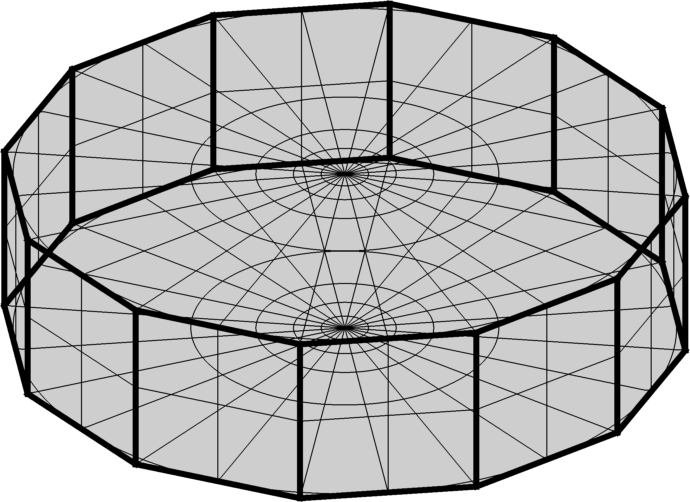
\includegraphics[width=2.8cm]{oR/Rod622} \qquad
    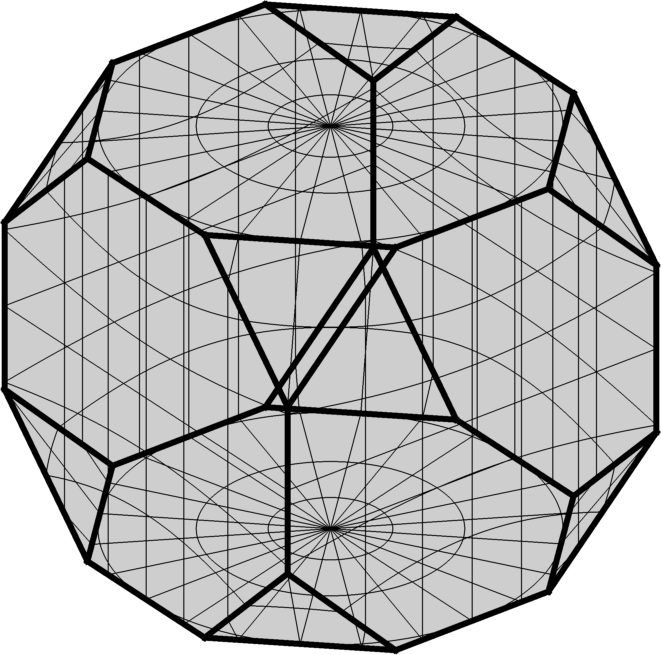
\includegraphics[width=2.8cm]{oR/Rod432}
  \end{center}

\end{frame}

\begin{frame}
  \frametitle{Fundamental Regions in Axis Angle Space}

  \begin{minipage}[c]{0.19\linewidth}
    \centering
    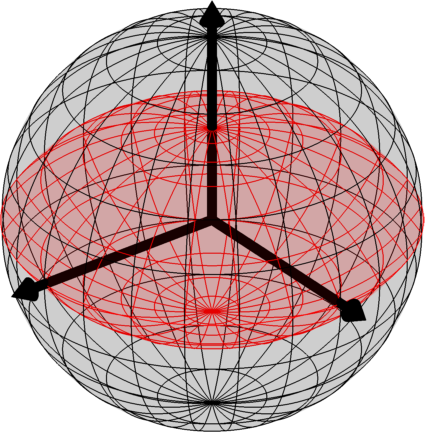
\includegraphics[width=\textwidth]{oR/oR112}
    2
  \end{minipage}
  \begin{minipage}[c]{0.19\linewidth}
    \centering
    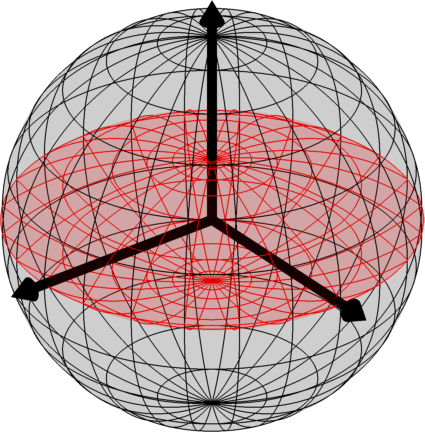
\includegraphics[width=\textwidth]{oR/oR3}
    3
  \end{minipage}
  \begin{minipage}[c]{0.19\linewidth}
    \centering
    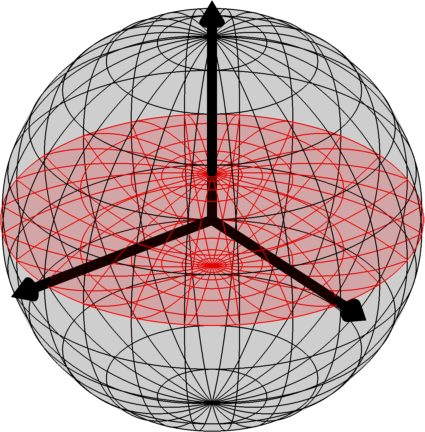
\includegraphics[width=\textwidth]{oR/oR4}
    4
  \end{minipage}
  \begin{minipage}[c]{0.19\linewidth}
    \centering
    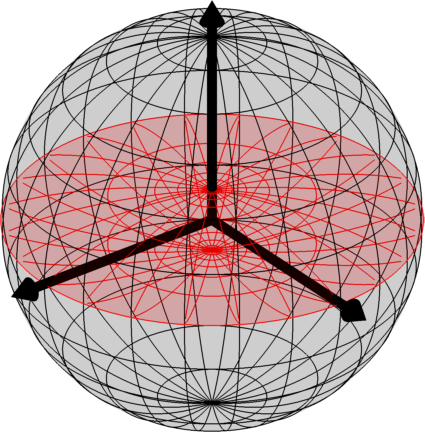
\includegraphics[width=\textwidth]{oR/oR6}
    6
  \end{minipage}
  \begin{minipage}[c]{0.19\linewidth}
    \centering
    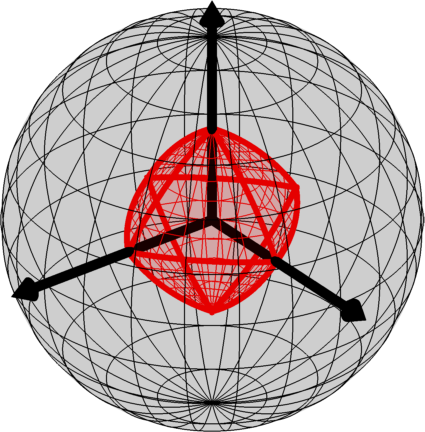
\includegraphics[width=\textwidth]{oR/oR23}
    23
  \end{minipage}

  \bigskip

  \begin{minipage}[c]{0.19\linewidth}
    \centering
    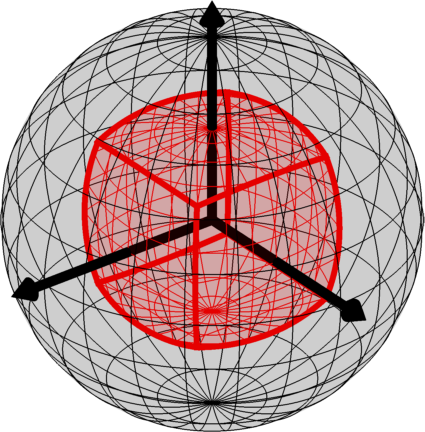
\includegraphics[width=\textwidth]{oR/oR222}
    222
  \end{minipage}
  \begin{minipage}[c]{0.19\linewidth}
    \centering
    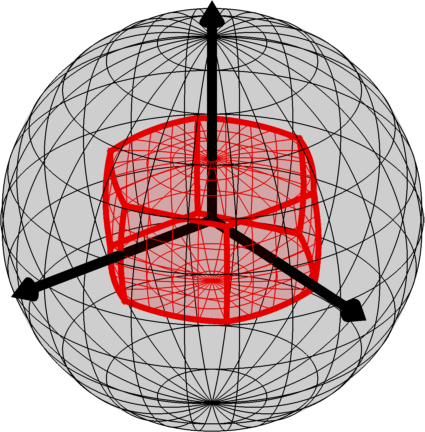
\includegraphics[width=\textwidth]{oR/oR321}
    321
  \end{minipage}
  \begin{minipage}[c]{0.19\linewidth}
    \centering
    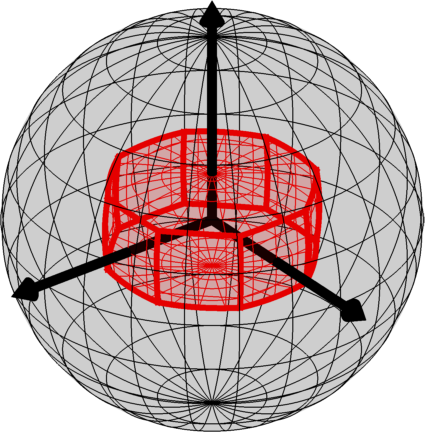
\includegraphics[width=\textwidth]{oR/oR422}
    422
  \end{minipage}
  \begin{minipage}[c]{0.19\linewidth}
    \centering
    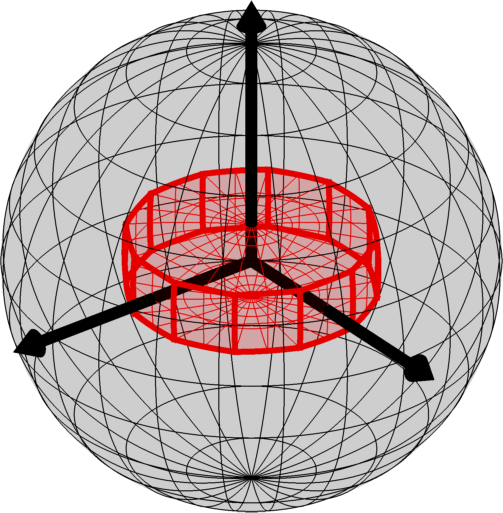
\includegraphics[width=\textwidth]{oR/oR622}
    622
  \end{minipage}
  \begin{minipage}[c]{0.19\linewidth}
    \centering
    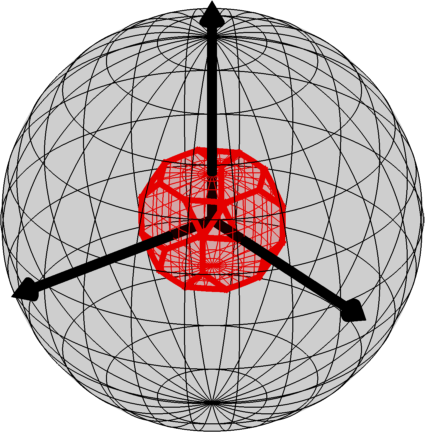
\includegraphics[width=\textwidth]{oR/oR432}
    432
  \end{minipage}
\end{frame}






\begin{frame}
  \frametitle{Pole Figures  (crystal directions in specimen coordinates)}

  \begin{overlayarea}{\textwidth}{7.8cm}
    \begin{itemize}
    \item $\vec h$ - crystal direction
    \paraitem $\mat S \vec h$ - crystallographic equivalent
    directions
    \paraitem $\mat O$ - orientation
  \end{itemize}

  
  \begin{block}{}
    $\implies$ crystallographic equivalent directions in specimen coordinates:
    $\ds \mat O \mat S \vec h, \quad \mat S \in \mathcal S $
  \end{block}

  \medskip
  
    Spherical plots of these directions are called \structure{pole figures}.

    \begin{itemize}
    \item every orientation appears $|\mathcal S \vec h|$ times
    \item if $\vec h$ and $-\vec h$ are symmetric only the upper hemisphere
      needs to be plotted
    \item pole figures reflects the macroscopic symmetries of the specimen
    \end{itemize}

    \medskip
    
    \only<1|handout=0>{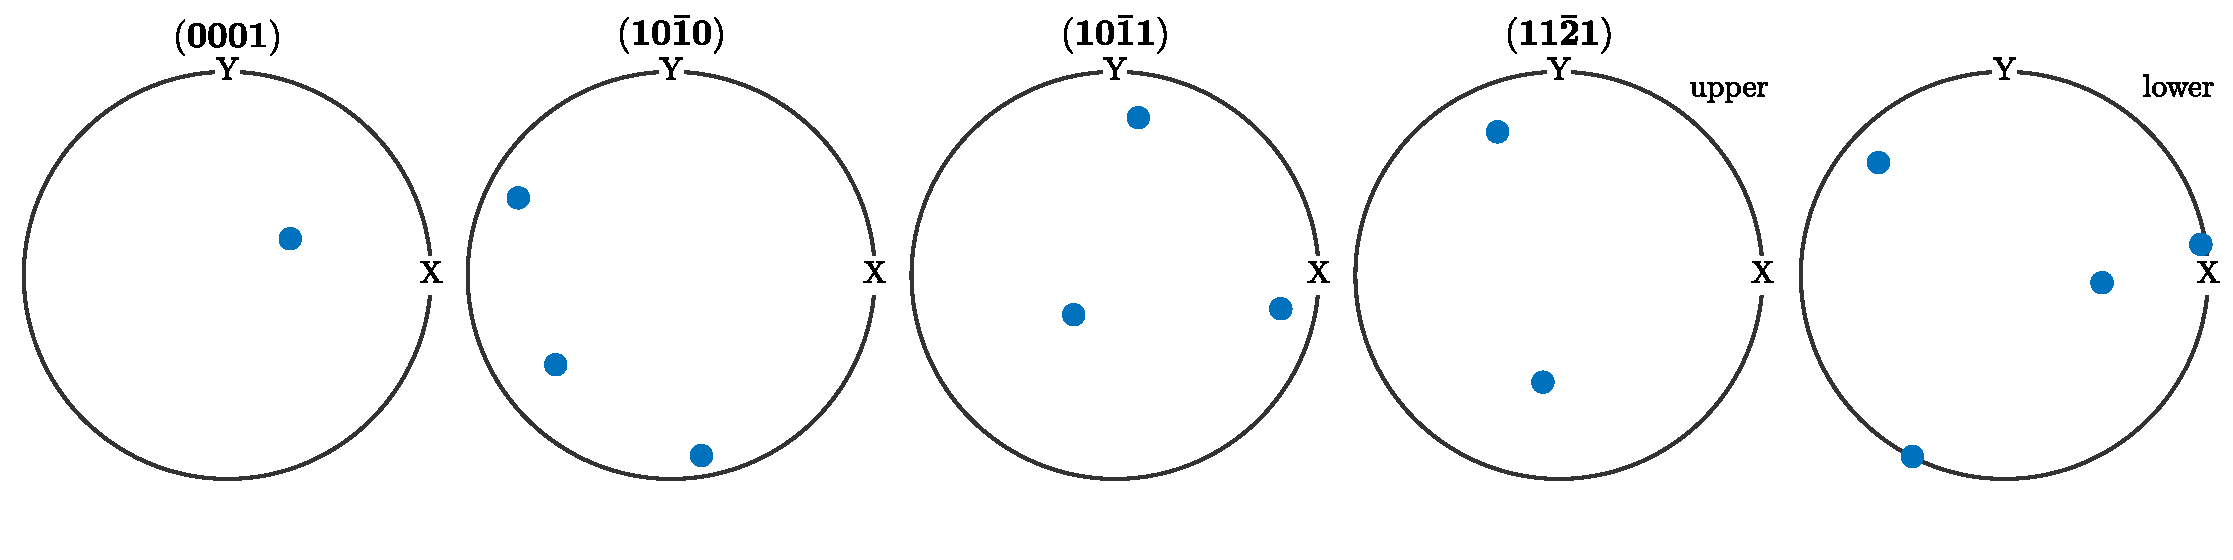
\includegraphics[width=\textwidth]{pic/pf_ori}}
    \only<2>{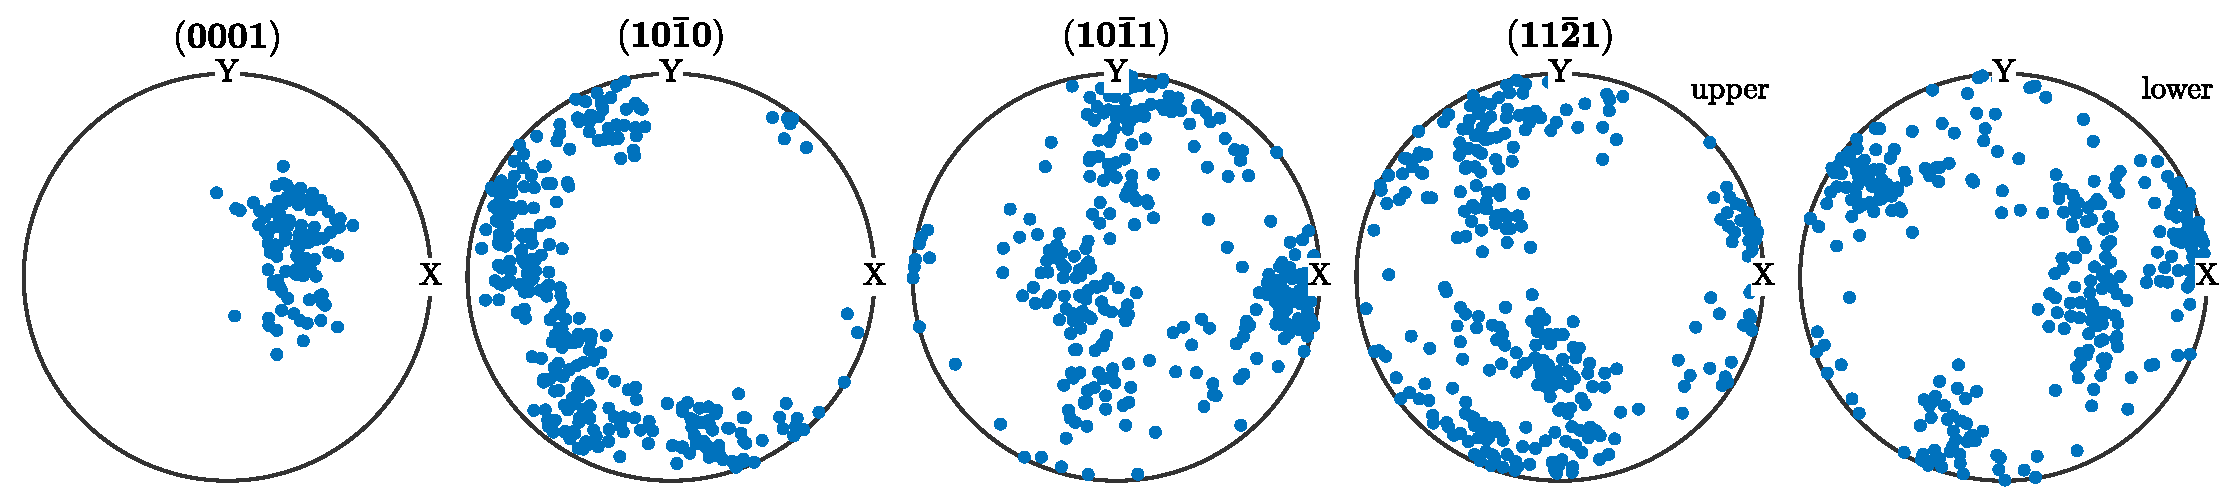
\includegraphics[width=\textwidth]{pic/pf_ori_dubna}}
  \end{overlayarea}
\end{frame}

\begin{frame}
  \frametitle{Inverse Pole Figures (specimen directions in crystal coordinates)}

    \begin{overlayarea}{\textwidth}{7.8cm}
    \begin{itemize}
    \item $\vec r$ - specimen direction
    \paraitem $\mat O$ - orientation
  \end{itemize}

  \begin{block}{}
    $\implies$ crystal directions pointing in direction $\vec r$:
    $\ds \mat S \mat O^{-1}  \vec r, \quad \mat S \in \mathcal S $
  \end{block}

      \medskip
  
    Spherical plots of these directions are called \structure{inverse pole figures}.

        \medskip
    
    \begin{itemize}
    \item every orientation appears $|\mathcal S|$ times
      \only<3>{\paraitem only the fundamental sector needs to be plotted}
    \end{itemize}

    \only<1|handout=0>{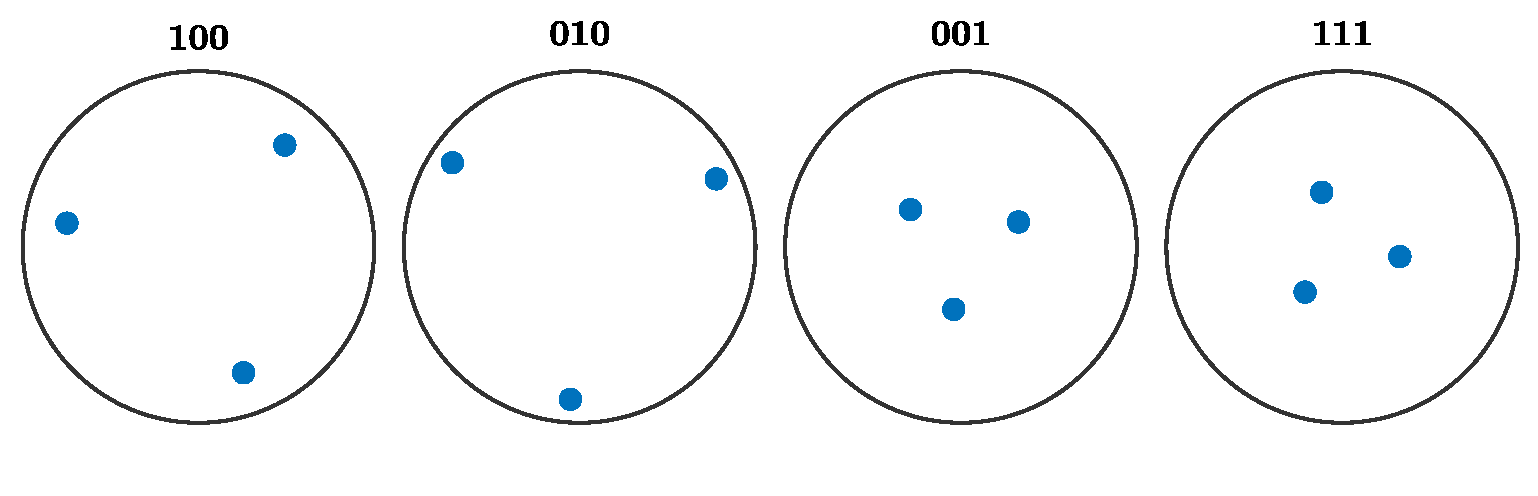
\includegraphics[width=\textwidth]{pic/ipf_ori}}
    \only<2|handout=0>{\centering 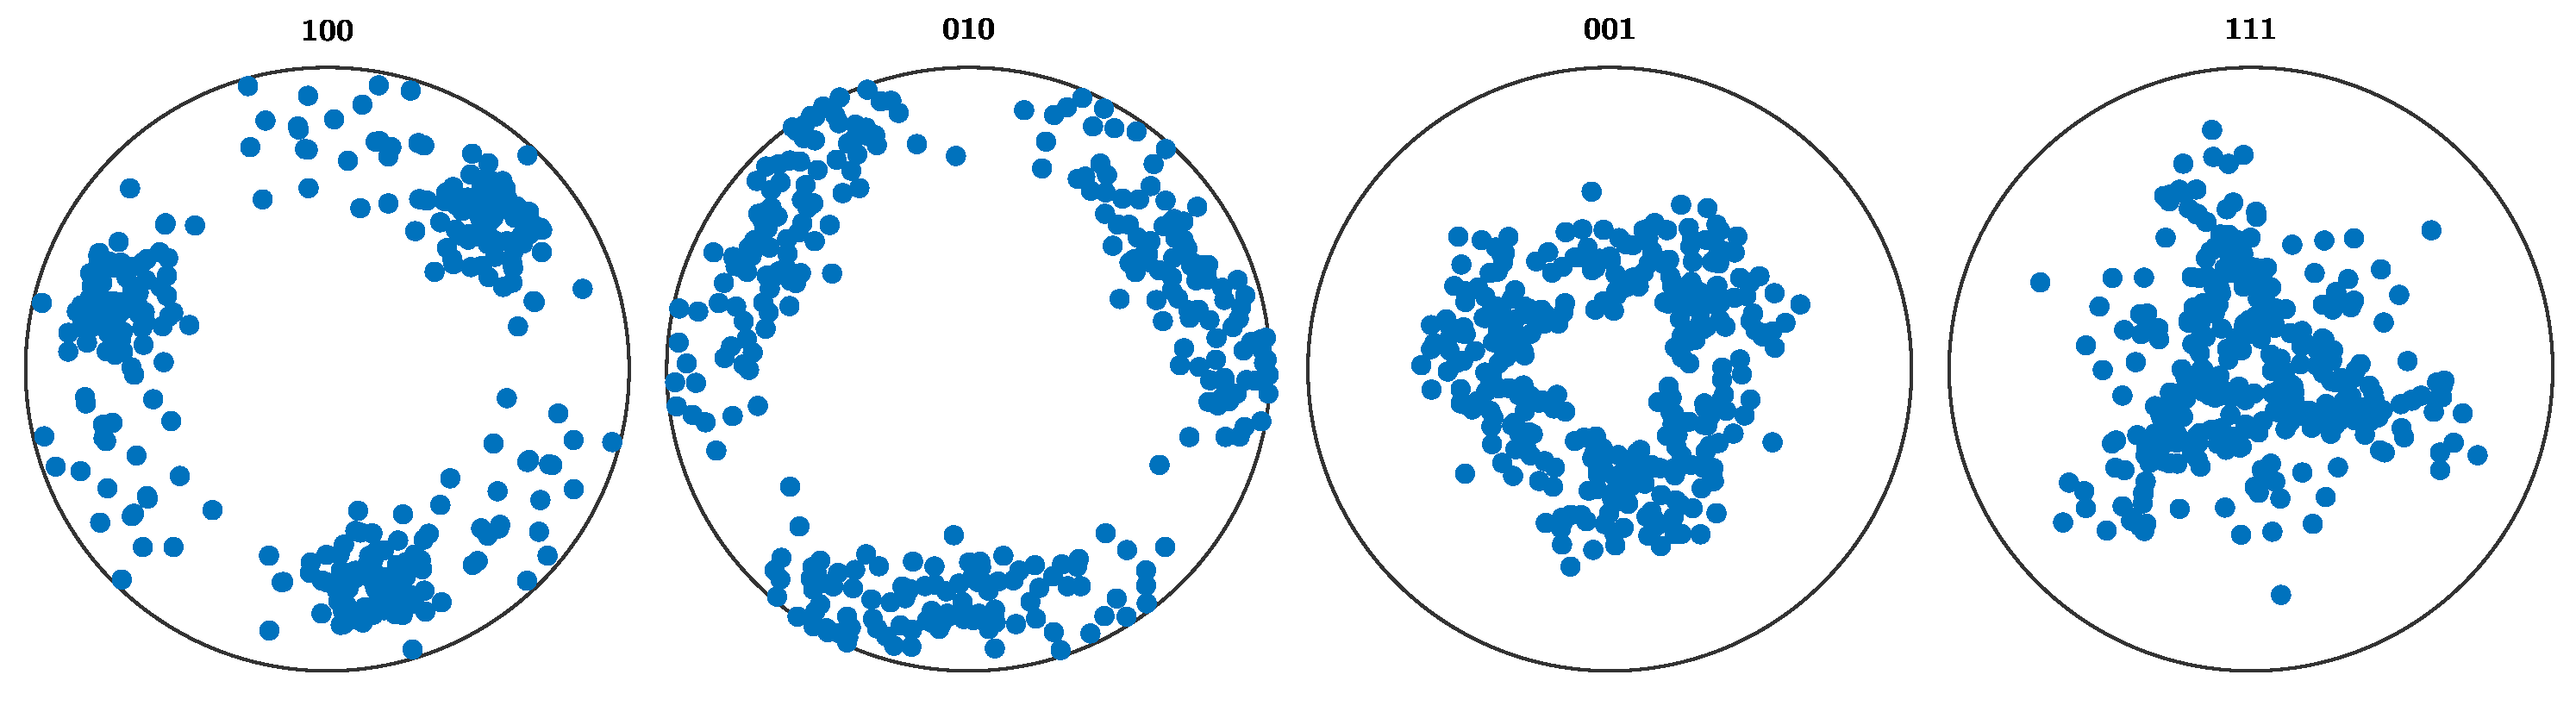
\includegraphics[width=\textwidth]{pic/ipf_ori_dubna_complete}}
    \only<3>{\centering 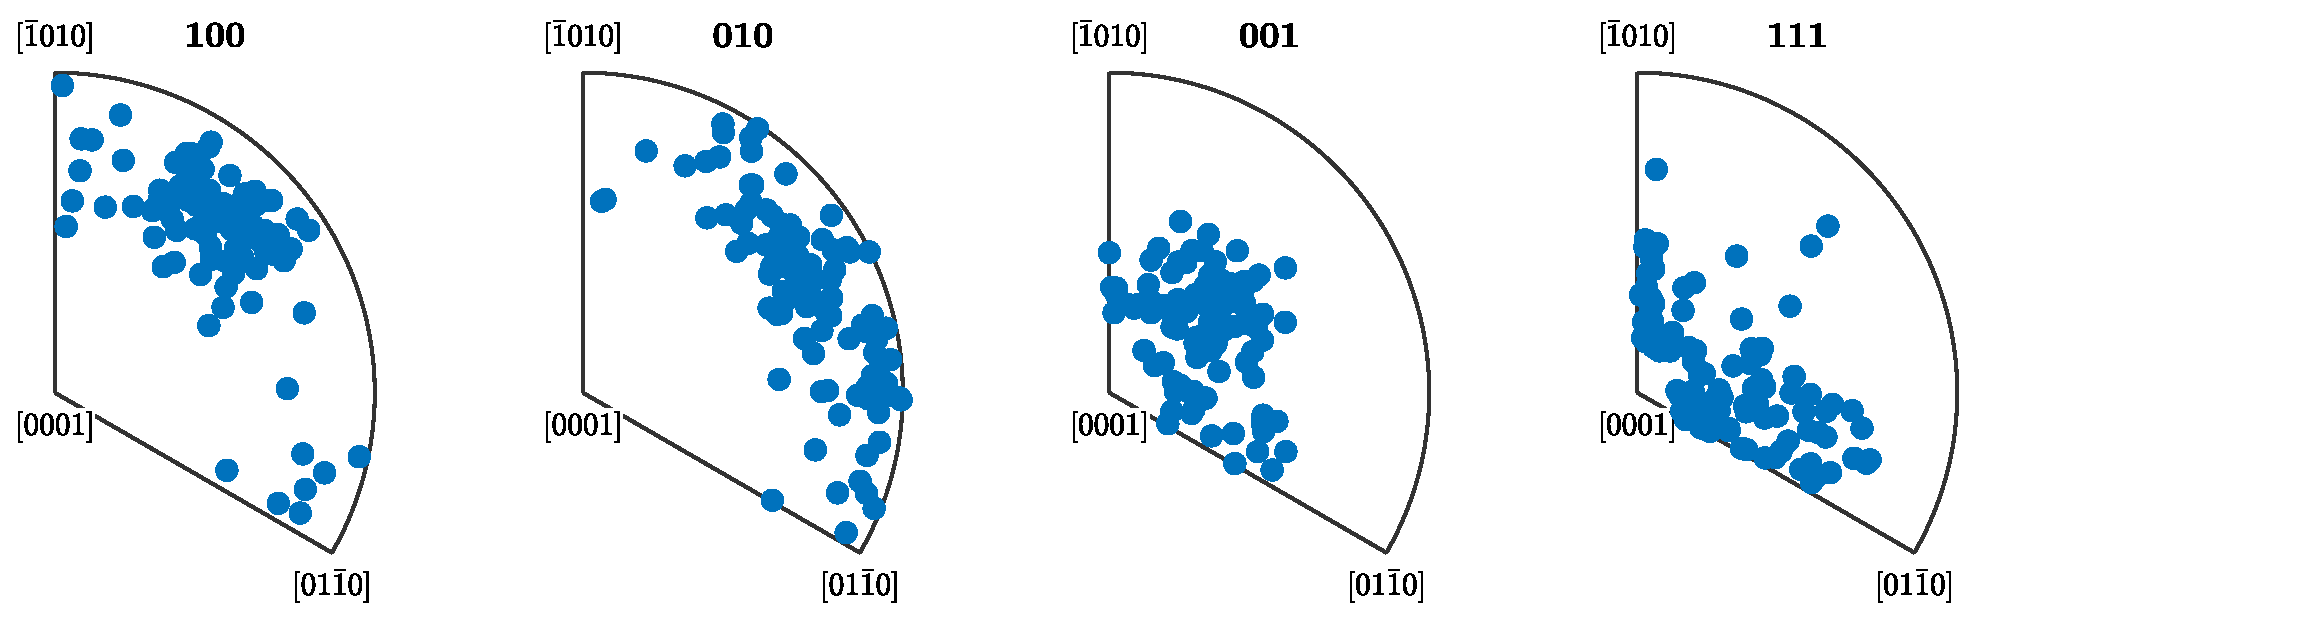
\includegraphics[height=4.5cm]{pic/ipf_ori_dubna}}
  \end{overlayarea}
\end{frame}

\begin{frame}[fragile]
  \frametitle{MTEX}

\begin{lstlisting}[style=input]
cs = crystalSymmetry.load('quartz');
ori = orientation.rand(100,cs);

% pole figure plots
h = Miller(1,1,-2,0,cs)
plot(ori * h.symmetrise)
plotPDF(ori,h)

% inverse pole figure plots
r = vector3d.Z
plot(inv(ori.symmetrise) * r)
plotIPDF(ori,r)
\end{lstlisting}


\end{frame}



\begin{frame}
  \frametitle{Visualizing Orientations}

  \begin{columns}
    \begin{column}{0.26\textwidth}
      \vspace{-0.5cm}
      \begin{block}{3d plots}
        \begin{itemize}
        \item<+-> Euler angle space
        \item<+-> axis angle space
        \item<+-> Rodrigues space
        \end{itemize}
      \end{block}

      \begin{block}{section plots}
        \begin{itemize}
        \item<+-> Euler angle sections
        \item<+-> axis angle sections
        \item<+-> sigma sections
        \end{itemize}
      \end{block}

      \begin{block}{projection plots}
        \begin{itemize}
        \item<+-> pole figures
        \item<+-> inverse pole figures
        \end{itemize}
      \end{block}
    \end{column}
    \begin{column}{0.7\textwidth}
      \begin{overlayarea}{\textwidth}{0.95\textheight}
          \begin{onlyenv}<1|handout:0>
            \vspace{0.75cm}
            \centerline{
              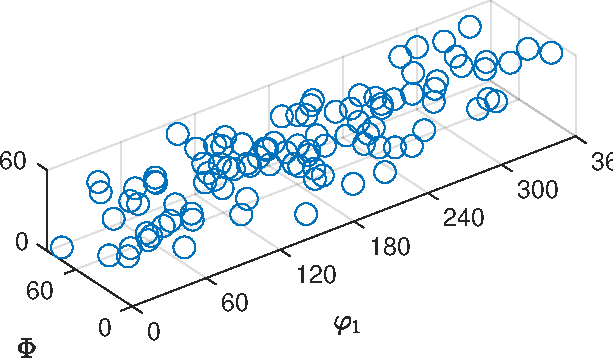
\includegraphics[width=0.9\textwidth]{pic/Euler3d}}
          \end{onlyenv}
          \begin{onlyenv}<2|handout:0>
            \vspace{0.5cm}
            \centerline{
              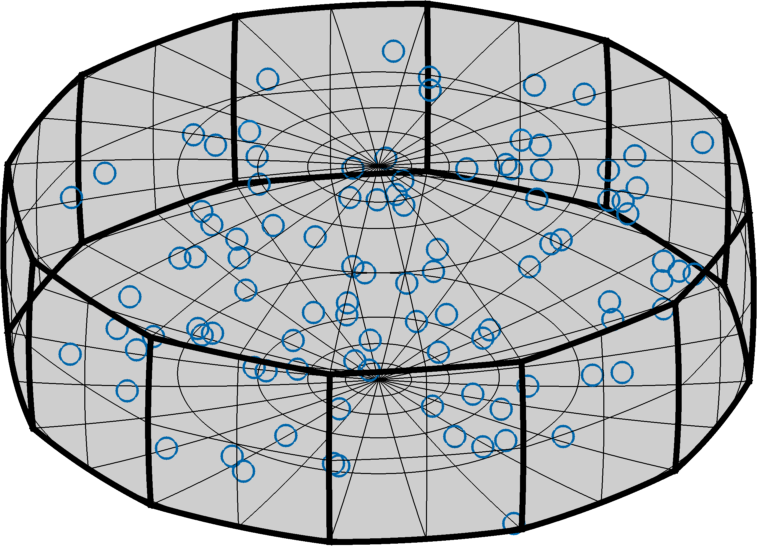
\includegraphics[width=0.8\textwidth]{pic/AxisAngle3d.png}}
          \end{onlyenv}
          \begin{onlyenv}<3|handout:0>
            \vspace{0.5cm}
            \centerline{
              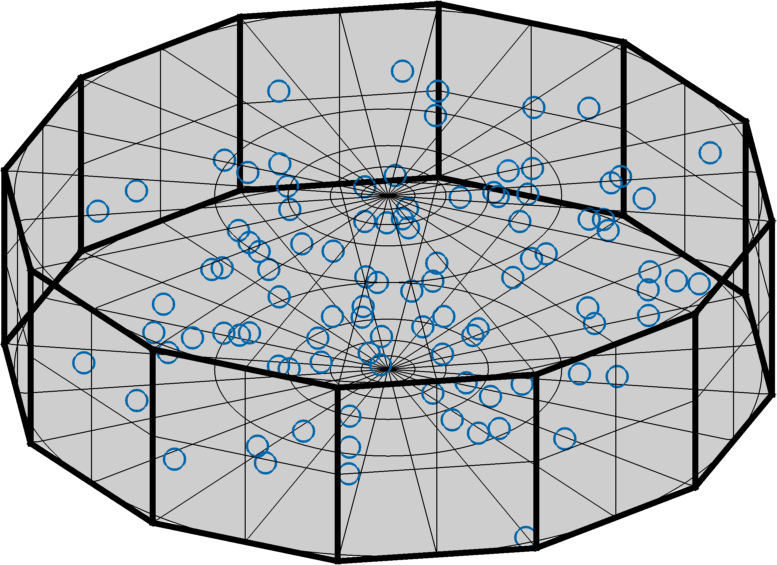
\includegraphics[width=0.8\textwidth]{pic/rodrigues3d}}
          \end{onlyenv}
          \begin{onlyenv}<4|handout:0>
            \centerline{
              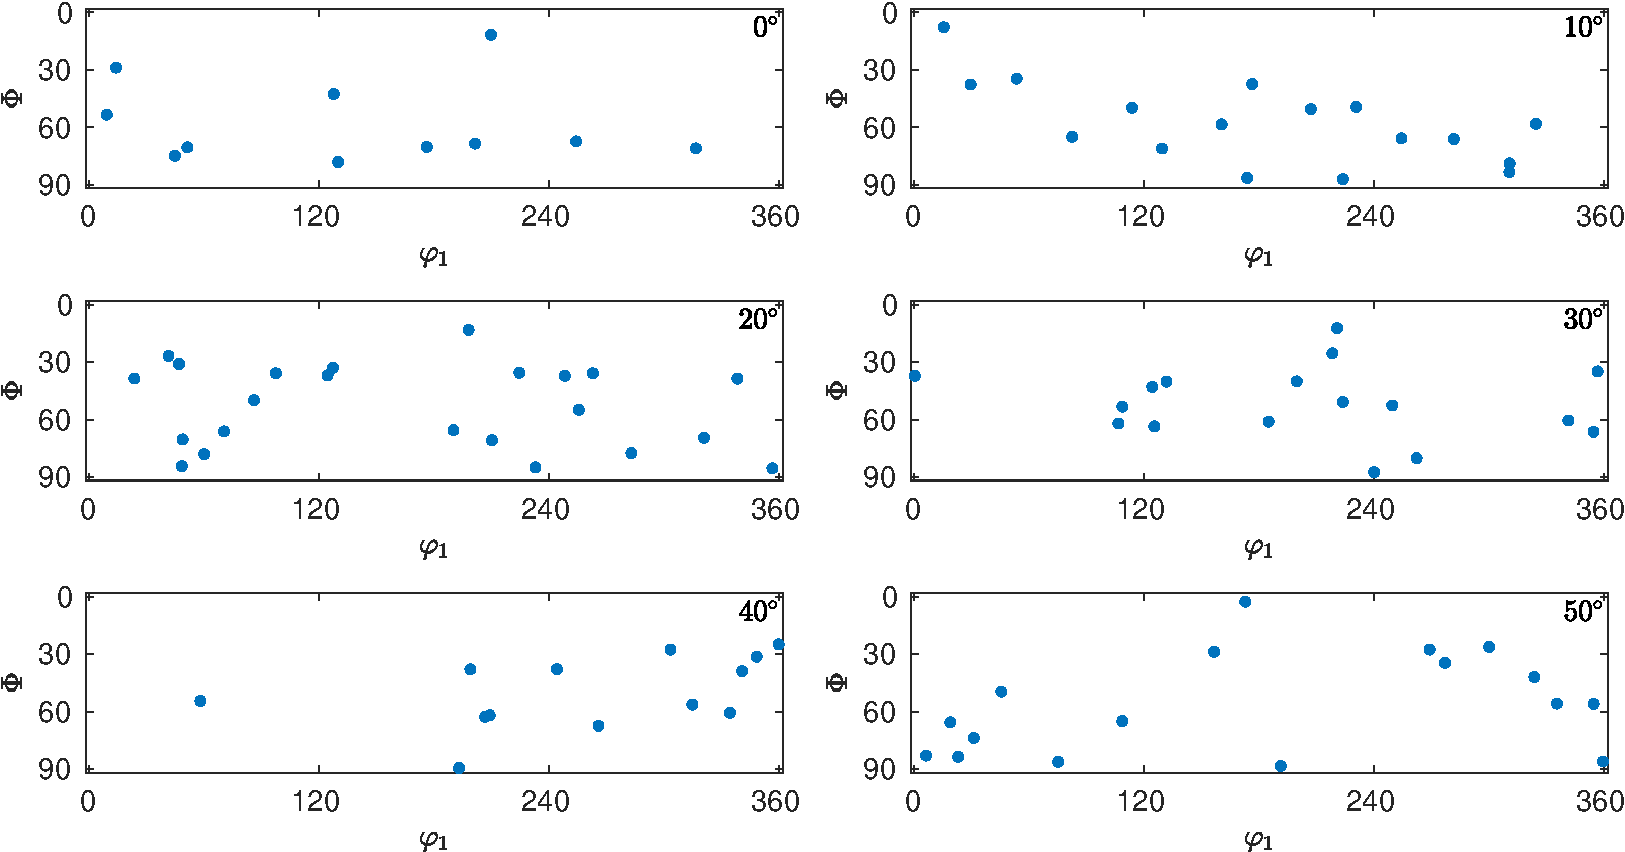
\includegraphics[width=\textwidth]{pic/EulerSection}}
          \end{onlyenv}
          \begin{onlyenv}<5|handout:0>
            \centerline{
              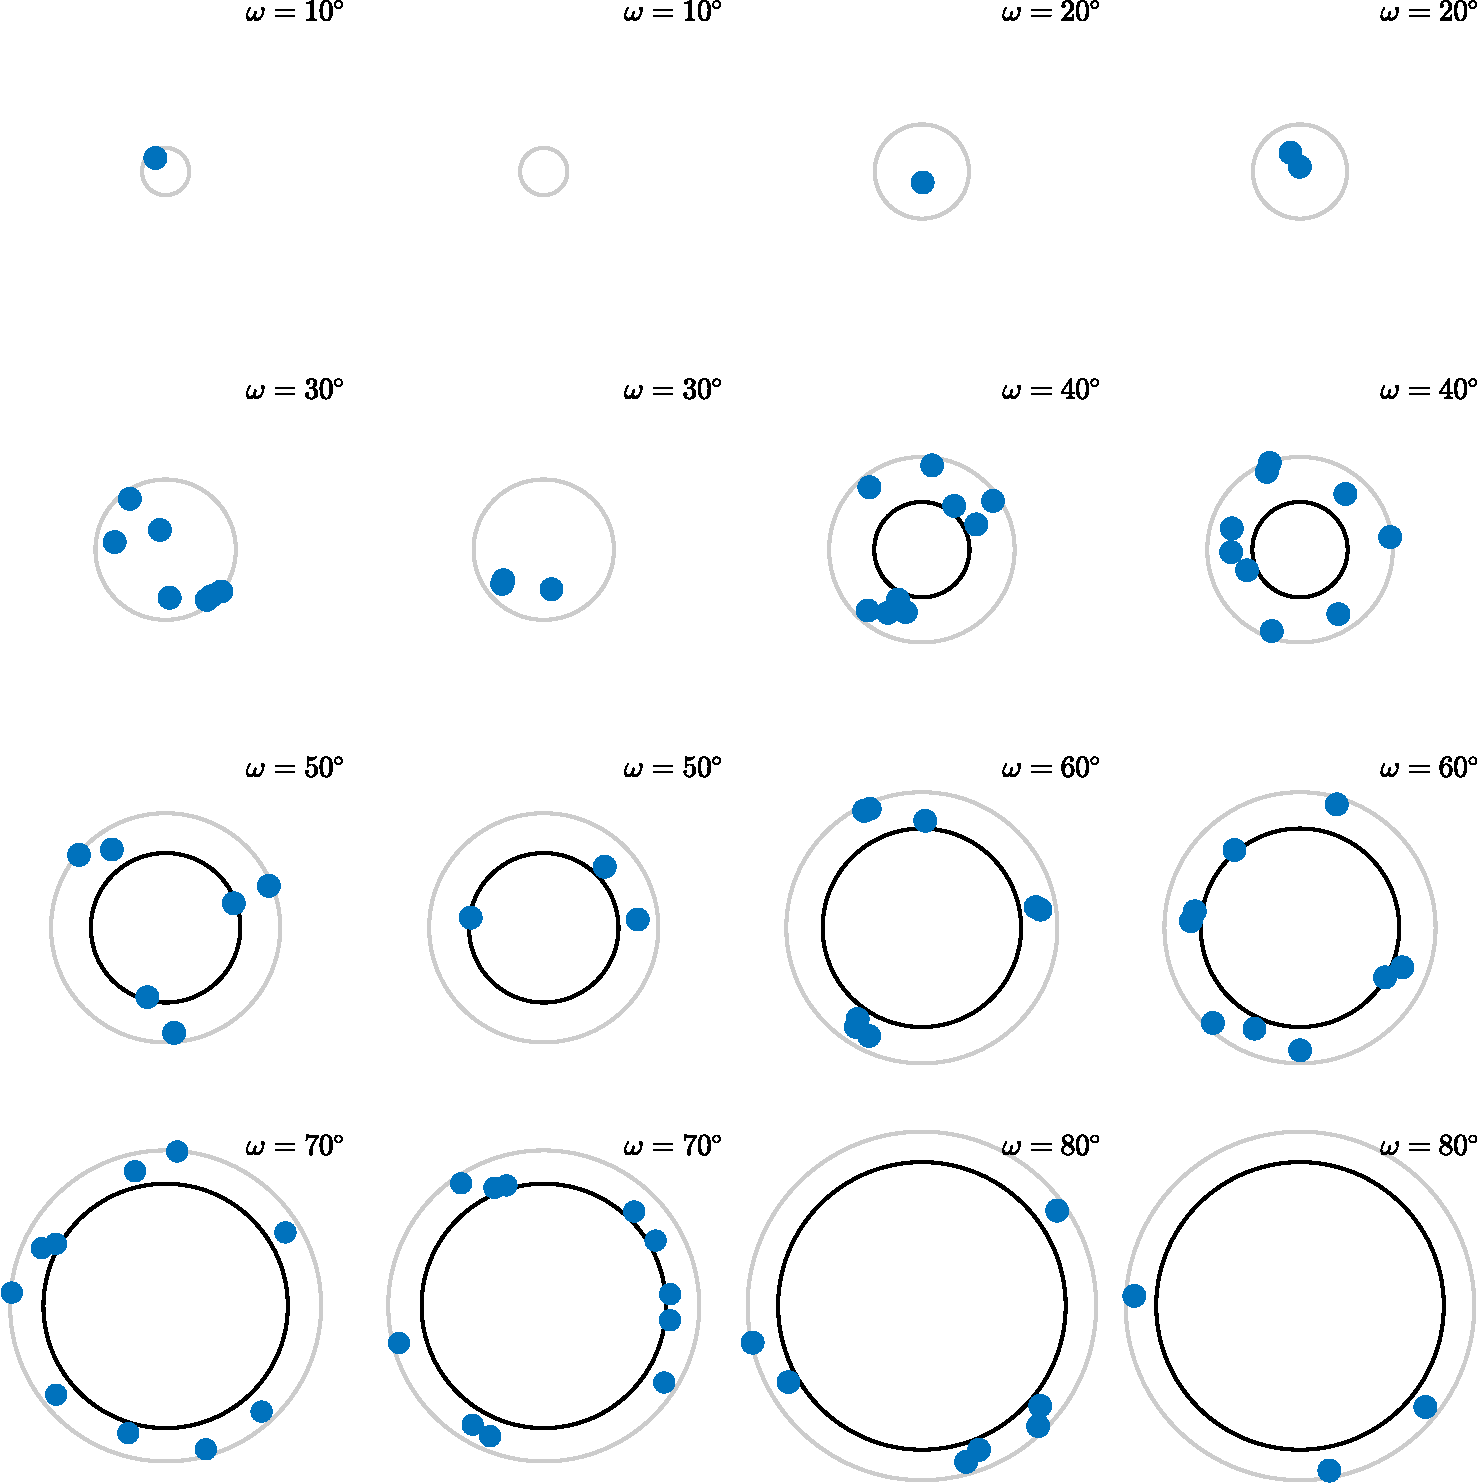
\includegraphics[height=0.9\textheight]{pic/AxisAngleSection}}
          \end{onlyenv}
          \begin{onlyenv}<6>
            \centerline{
              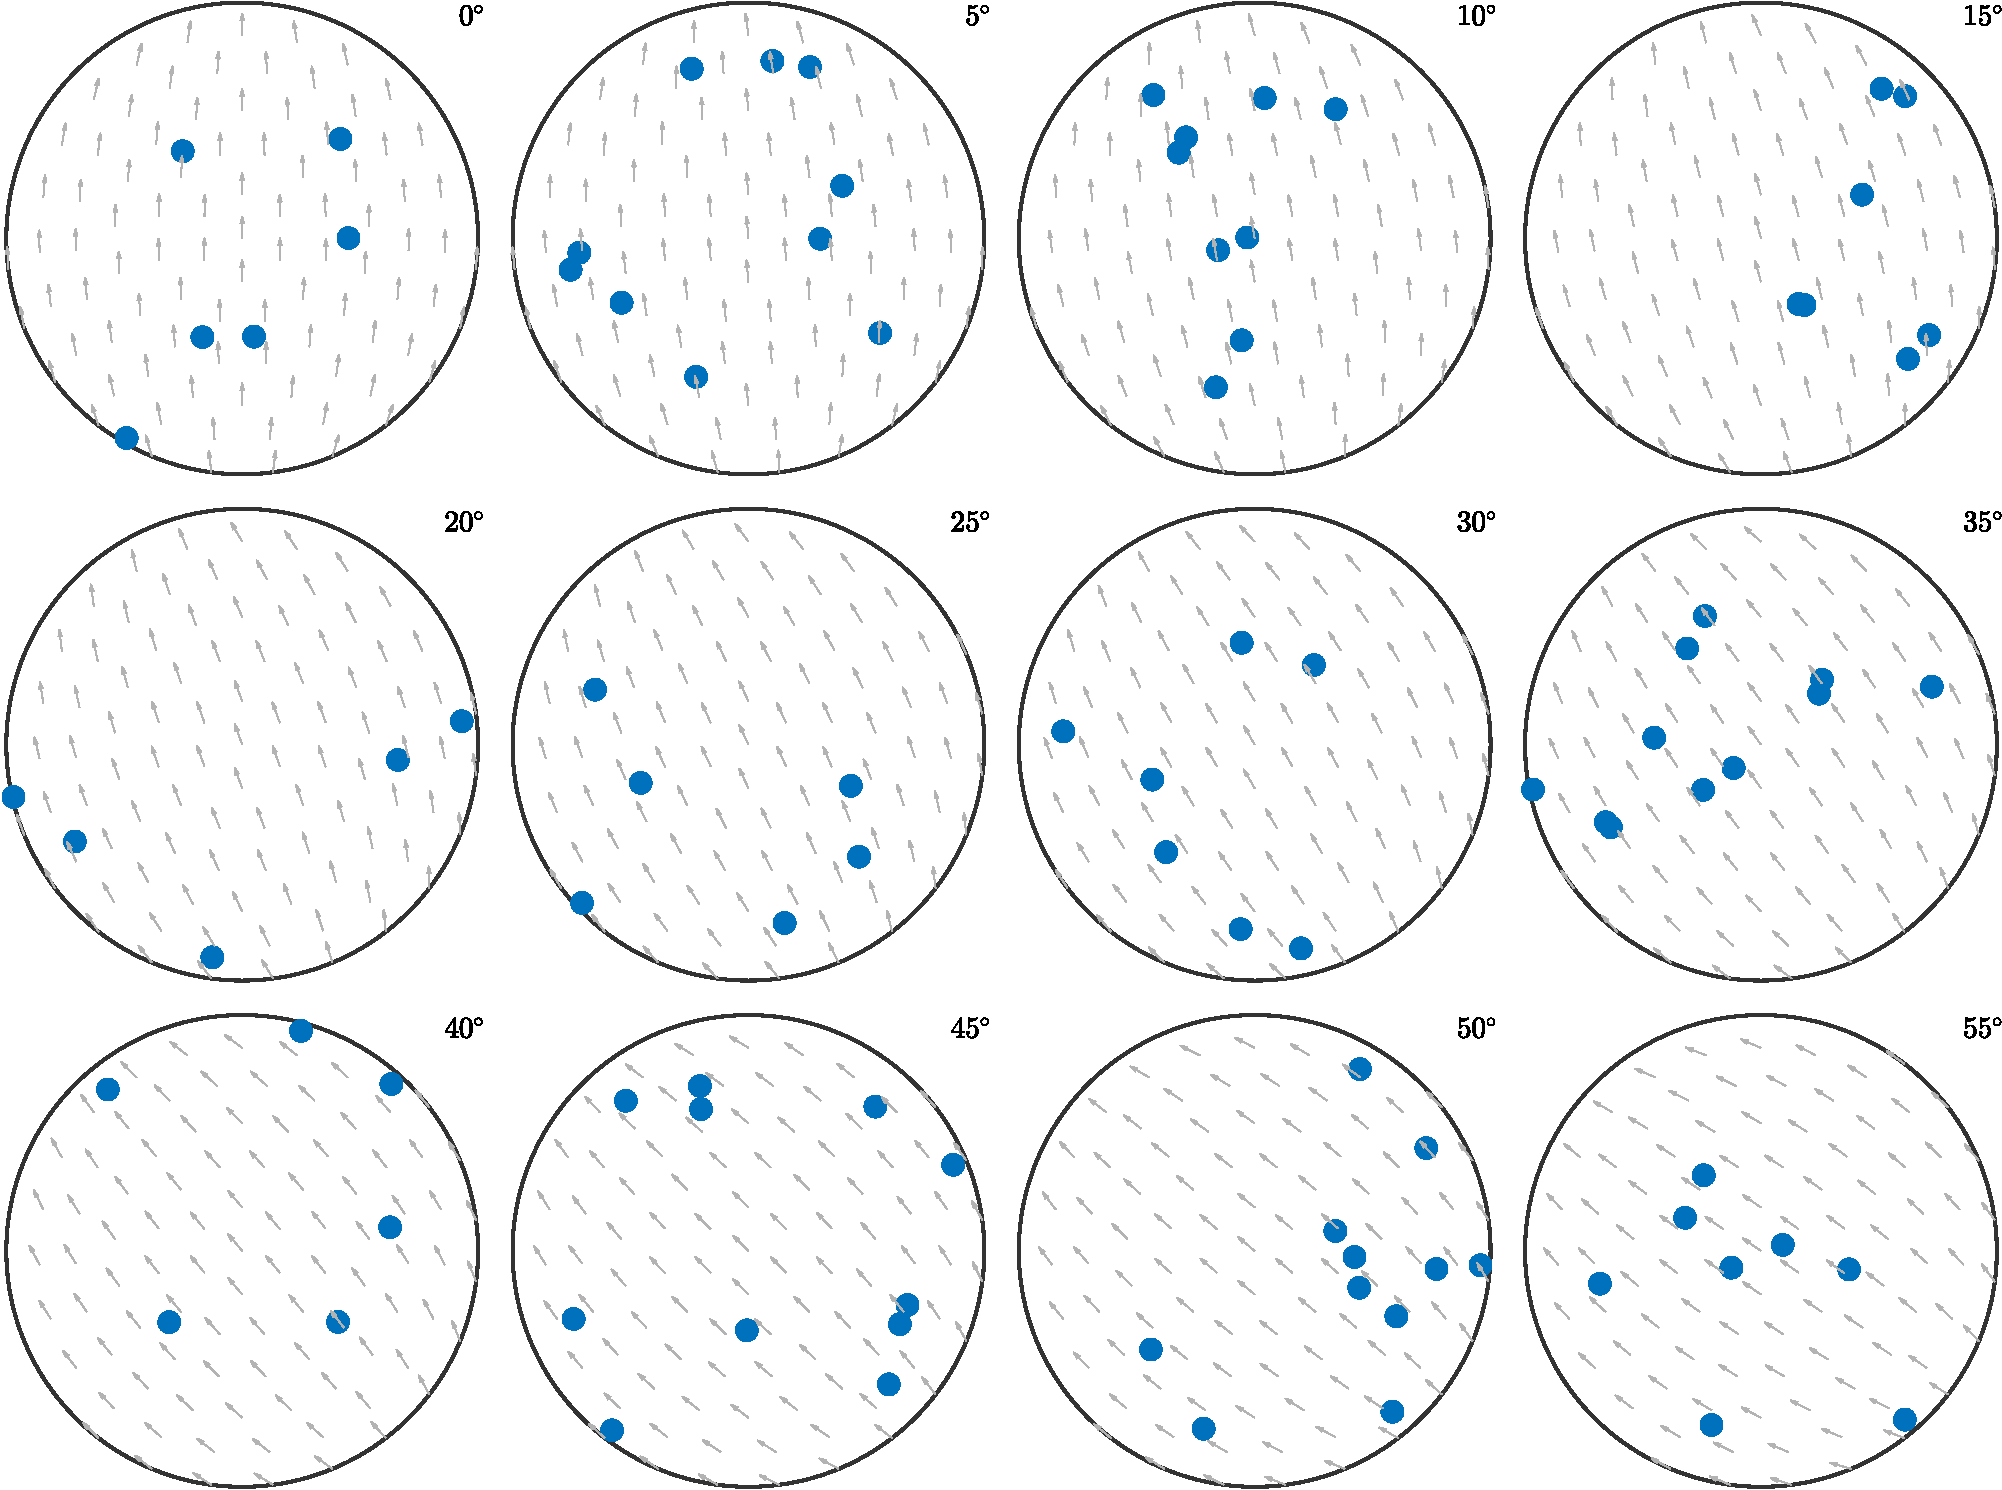
\includegraphics[width=\textwidth]{pic/SigmaSection}}
          \end{onlyenv}
          \begin{onlyenv}<7|handout:0>
            \centerline{
              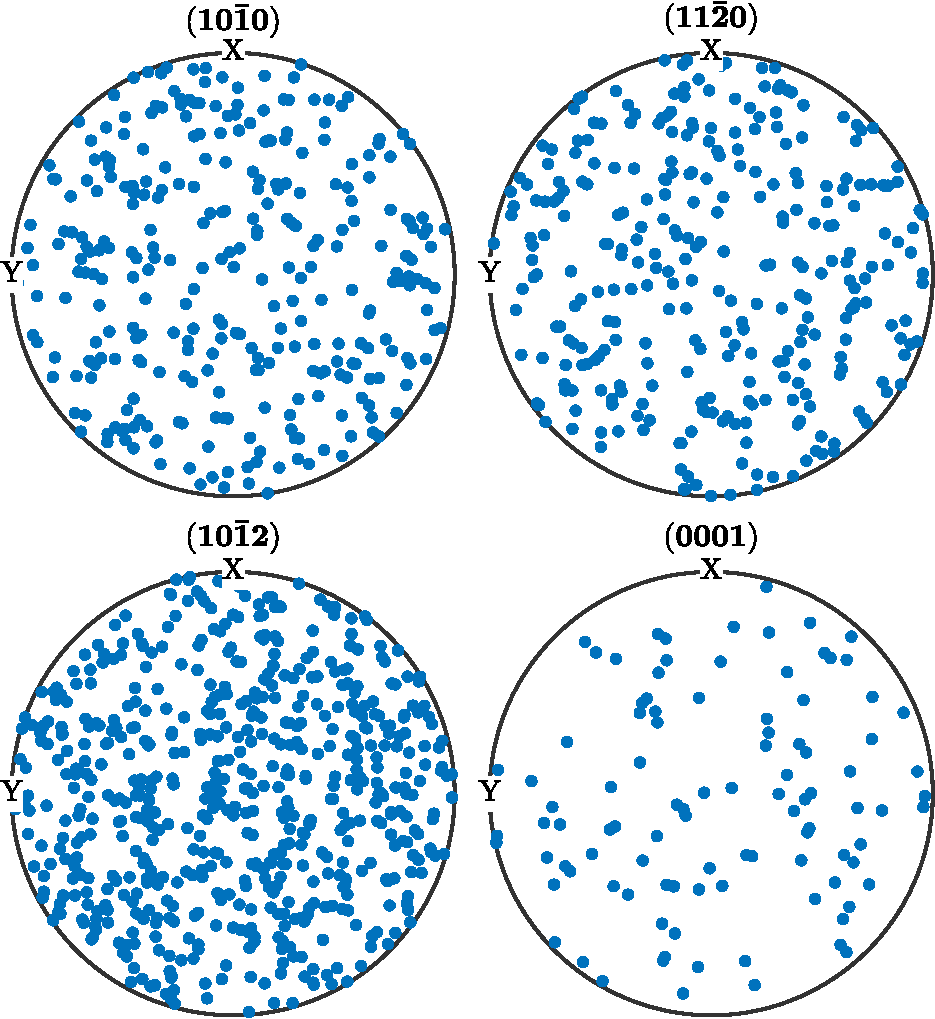
\includegraphics[height=0.9\textheight]{pic/PFRandom}}
          \end{onlyenv}
          \begin{onlyenv}<8|handout:0>
            \centerline{
              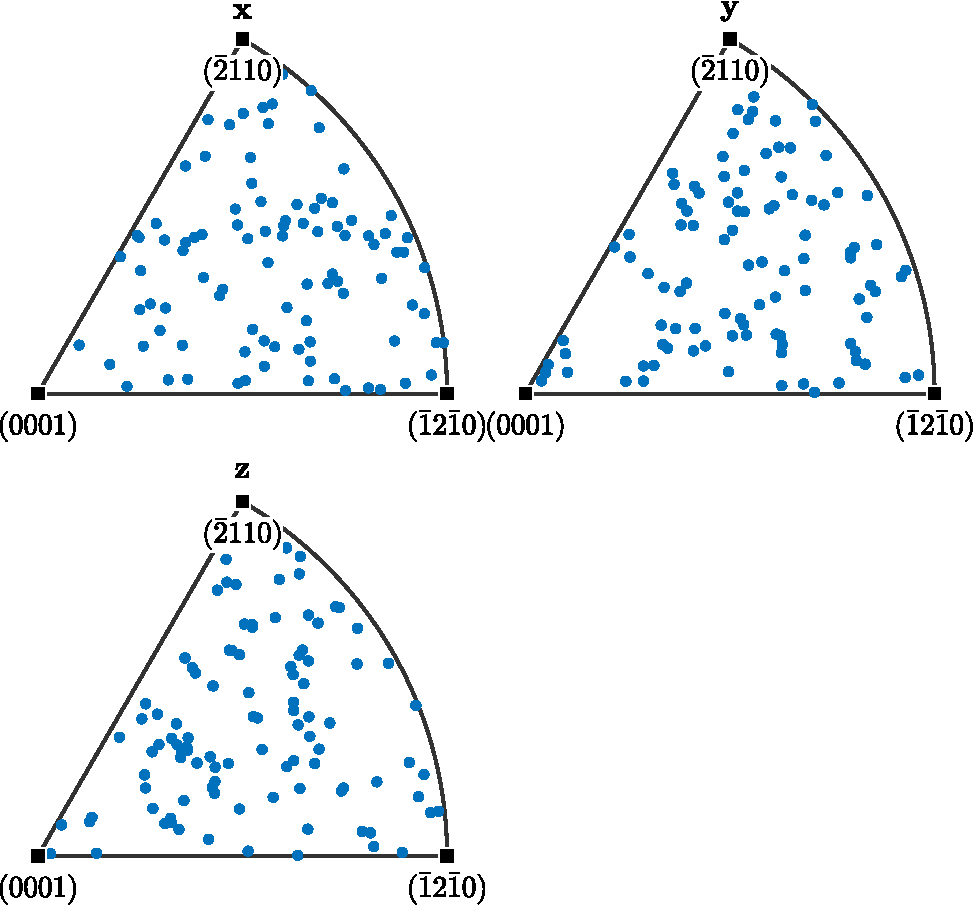
\includegraphics[height=0.9\textheight]{pic/IPFRandom}}
          \end{onlyenv}
      \end{overlayarea}
    \end{column}
  \end{columns}

\end{frame}


\begin{frame}[fragile]
  \frametitle{MTEX}

\begin{lstlisting}[style=input]
% some random orientations
cs = crystalSymmetry('cubic')
ori = orientation.rand(100,cs)

% 3d plots
plot(ori) % Euler angle plots
plot(ori,'axisAngle')
plot(ori,'Rodrigues')

% sections
plotSection(ori,'phi2',(0:10:50)*degree)
plotSection(ori,'sigma','sections',12)
plotSection(ori,'axisAngle')
\end{lstlisting}



\end{frame}


\begin{frame}[fragile]
  \frametitle{Fibers of Orientations}

  \begin{columns}
    \begin{column}{0.5\textwidth}
      \begin{overlayarea}{\textwidth}{0.93\textheight}

        The shortest line between two orientations \texttt{ori1} and
        \texttt{ori2} is called fibre.

        \begin{onlyenv}<3|handout:0>
\begin{lstlisting}[style=input]
f = fibre(o1,o2)
\end{lstlisting}
  \vspace{-0.3cm}
  \begin{lstlisting}[style=output]
f = /+fibre+/ (/+432+/ -> xyz (222))

 h || r: (011) || (0,0,1)
 o1 -> o2: (0°,45°,0°) -> (35°,45°,0°)
  \end{lstlisting}
\end{onlyenv}
%
\begin{onlyenv}<4->
\begin{lstlisting}[style=input]
f = fibre(o1,o2,'full')
\end{lstlisting}
\end{onlyenv}
  \vspace{-0.3cm}
\begin{onlyenv}<4|handout:0>
  \begin{lstlisting}[style=output]
f = /+fibre+/ (/+432+/ -> xyz (222))

 h || r: (011) || (0,0,1)
\end{lstlisting}
\end{onlyenv}
%
\begin{onlyenv}<5->
\begin{lstlisting}[style=input]
f.symmetrise
\end{lstlisting}
\end{onlyenv}
\vspace{-0.3cm}
\begin{onlyenv}<5|handout:0>
\begin{lstlisting}[style=output]
f = /+fibre+/ (show methods, plot)
  size: 12 x 1
  crystal symmetry: 432 specimen
  symmetry: 222
\end{lstlisting}
\end{onlyenv}
%
\begin{onlyenv}<6->
\begin{lstlisting}[style=input]
f = fibre.beta(cs,ss)
\end{lstlisting}
\end{onlyenv}
%
\begin{onlyenv}<7->

  The full fiber is characterized by a crystal direction $(hk\ell)$ and a
  specimen direction $(xyz)$ as all orientations \texttt{ori} satisfying

  \begin{equation*}
    \mathtt{ori} * (hk\ell) = (xyz)
  \end{equation*}

\begin{lstlisting}[style=input]
fibre(Miller(1,1,1,cs),zvector)
\end{lstlisting}
\end{onlyenv}
\begin{onlyenv}<8-> \vspace{-0.1cm}
\begin{lstlisting}[style=input]
f = fibre.fit(ori)
\end{lstlisting}
\end{onlyenv}
\vspace{-0.1cm}
\begin{onlyenv}<9->
\begin{lstlisting}[style=input]
angle(ori,f)
\end{lstlisting}
\end{onlyenv}
\end{overlayarea}
\end{column}
\begin{column}{0.44\textwidth}
  \begin{overlayarea}{\textwidth}{0.95\textheight}
     \vspace{-0.5cm}
    \begin{onlyenv}<1->
\begin{lstlisting}[style=input]
cs = crystalSymmetry('432')
ss = specimenSymmetry('222')
o1 = orientation.goss(cs,ss)
\end{lstlisting}
    \end{onlyenv}
        %
    \begin{onlyenv}<2->
      \vspace{-0.3cm}
\begin{lstlisting}[style=input]
o2 = orientation.brass(cs,ss)
\end{lstlisting}
    \end{onlyenv}
        \begin{onlyenv}<1|handout:0>
      \begin{center}
        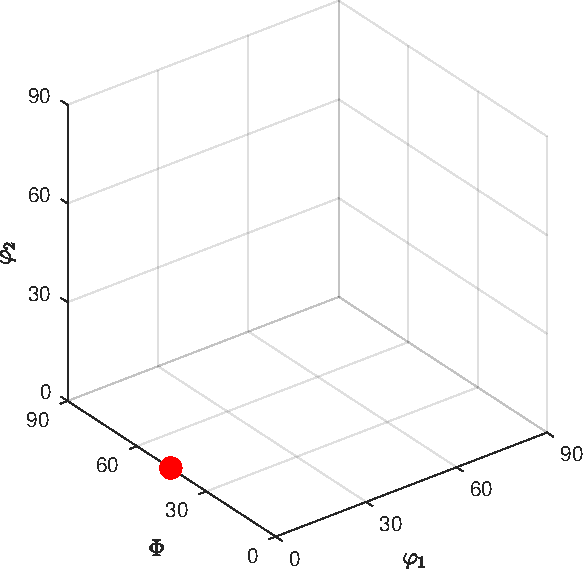
\includegraphics[width=0.8\textwidth]{pic/o1.pdf}
    \end{center}
    \end{onlyenv}
        \begin{onlyenv}<2|handout:0>
      \begin{center}
        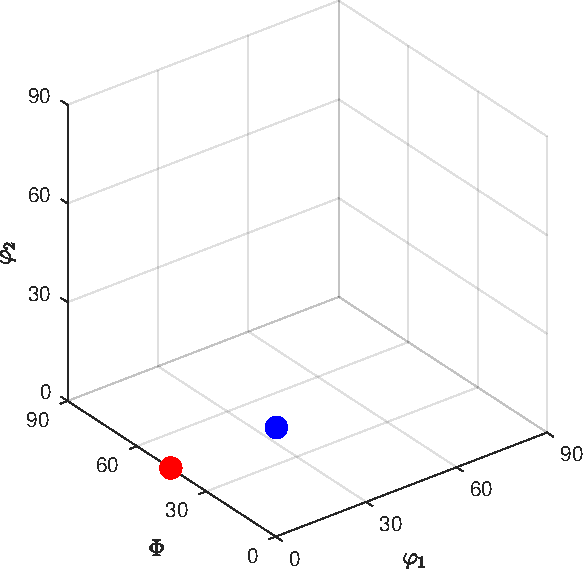
\includegraphics[width=0.8\textwidth]{pic/o2.pdf}
      \end{center}
    \end{onlyenv}
    \begin{onlyenv}<3|handout:0>
      \begin{center}
        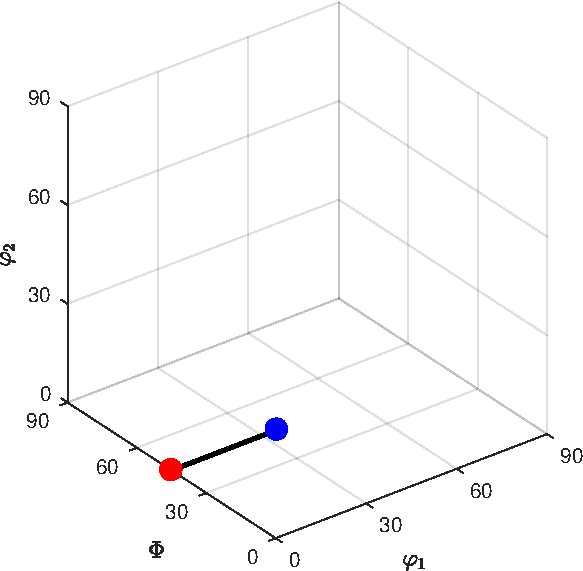
\includegraphics[width=0.8\textwidth]{pic/fibre1.pdf}
      \end{center}
    \end{onlyenv}
    \begin{onlyenv}<4|handout:0>
      \begin{center}
        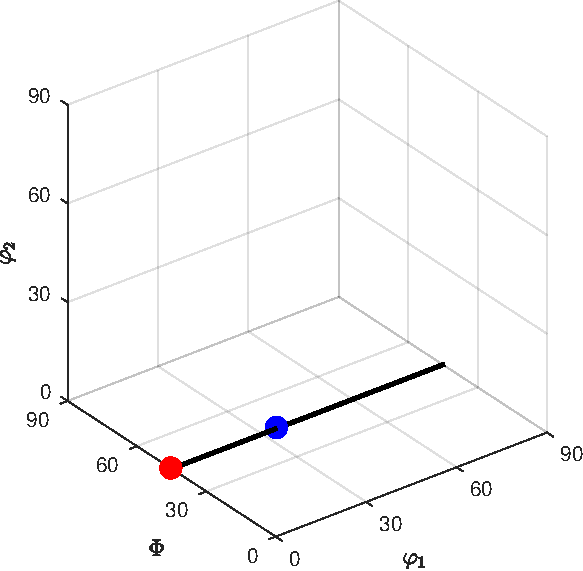
\includegraphics[width=0.8\textwidth]{pic/fibreFull.pdf}
      \end{center}
    \end{onlyenv}
    \begin{onlyenv}<5|handout:0>
      \begin{center}
        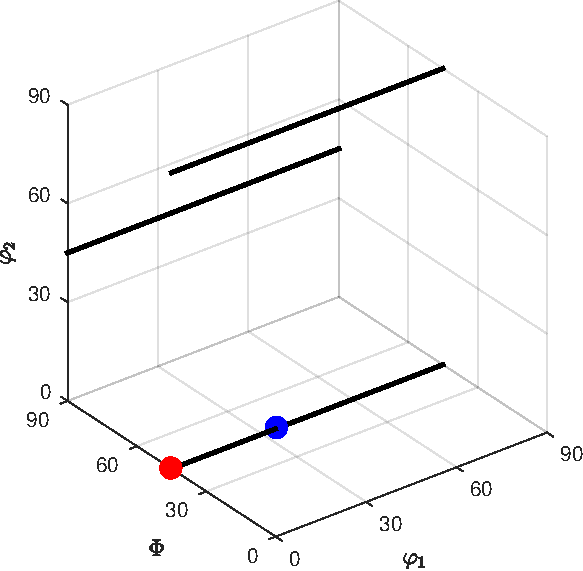
\includegraphics[width=0.8\textwidth]{pic/fibreSym.pdf}
      \end{center}
    \end{onlyenv}
    \begin{onlyenv}<6|handout:0>
      \begin{center}
        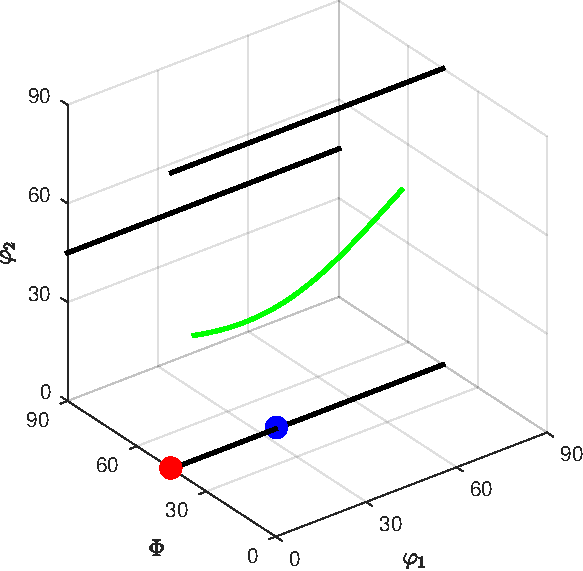
\includegraphics[width=0.8\textwidth]{pic/fibreBeta.pdf}
      \end{center}
    \end{onlyenv}
    \begin{onlyenv}<7->
      \begin{center}
        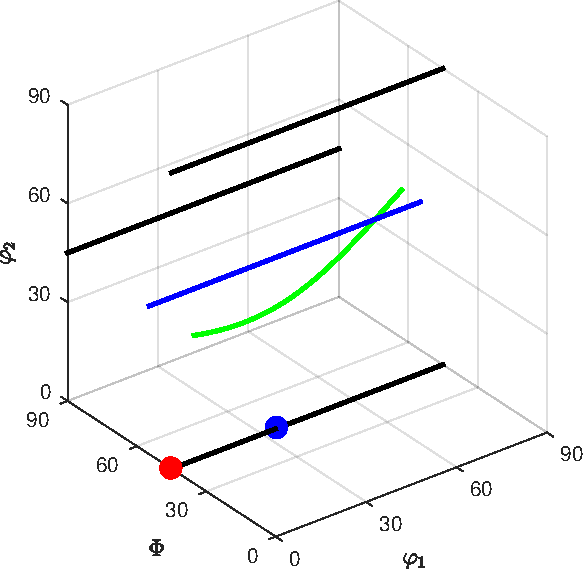
\includegraphics[width=0.8\textwidth]{pic/fibre2.pdf}
      \end{center}
    \end{onlyenv}
  \end{overlayarea}

\end{column}

\end{columns}
\end{frame}

\end{document}

\begin{frame}
  \frametitle{Colorizing Orientations}

  An \structure{orientation color key} is a map $\mathcal K$ that associates to
  each orientation $\mat O$ a color
  \begin{equation*}
    \mathcal K(\mat O) = (R,G,B).
  \end{equation*}

  \pause

  \begin{exampleblock}{The Euler angle color key}
    Let $\mat O = \mat O(\varphi_{1}, \Phi,\varphi_{2})$ an orientation with
    Euler angles $\varphi_{1}$, $\Phi$, $\varphi_{2}$ in the fundamental region
    $[0,\tilde \varphi_{1}]
    \times [0,\tilde \Phi] \times [0,\tilde \varphi_{2}]$. Then
    \begin{equation*}
      \mathcal K(\mat O) = \left( \frac{\varphi_{1}}{\tilde \varphi_{1}},
      \frac{\Phi}{\tilde \Phi},\frac{\varphi_{2}}{\tilde \varphi_{2}}\right)
    \end{equation*}
    defines the so called \emph{Euler angle color key}.
  \end{exampleblock}

  \bigskip
  \pause

    \structure{Properties of the Euler angle color key:}
  \begin{itemize}
  \item Different orientations have different colors.
  \item Different colors do not indicate different orientations, since the representation by Euler angles is not unique.
  \item For cubic symmetries the fundamental region is not of the form
    $[0,\tilde \varphi_{1}] \times [0,\tilde \Phi] \times [0,\tilde
    \varphi_{2}]$.

  \end{itemize}



\end{frame}

\begin{frame}
  \frametitle{Nice Color Keys}

  Requirements for a nice color key
  \begin{enumerate}
    \item<+-> similar orientations should have similar colors
    \item<+-> different orientations should have different colors
    \item<+-> important orientations should have simple colors
    \item<+-> contrast should indicate misorientation angle
  \end{enumerate}

  \begin{alertblock}{}<5->
    \alert{Theorem:} There is no such mapping.
  \end{alertblock}

  \medskip

  \pause

  We will drop requirement 2.


\end{frame}


\begin{frame}
  \frametitle{Inverse Pole Figure Color Keys}

  \structure{Idea:}
  \begin{itemize}
  \item<+-> fix a specimen direction, e.g., $\vec r = \vec Z$
  \item<+-> for an orientation $\mat O$ compute the inverse pole figure
    direction $\vec h = \mat O^{-1} \vec r$
  \item<+-> project $\vec h$ onto the fundamental sector $\mathbb
    S^{2}_{\mathcal S}$ corresponding to the symmetry group $\mathcal S$
  \item<+-> define a color key for the fundamental sector
    \begin{equation*}
      \mathcal K_{\mathbb
    S^{2}_{\mathcal S}}(\vec h) = (R,G,B)
    \end{equation*}
  \item<+-> set
    \begin{equation*}
      \mathcal K(\mat O)
      = \mathcal K_{\mathbb S^{2}_{\mathcal S}}(\vec h)
    \end{equation*}
  \end{itemize}




  \structure{Requirement:} The inverse pole figure color key needs to extent
  continuously to the whole sphere when applying symmetry operations.

\end{frame}

\begin{frame}
  \frametitle{IPF Color Keys for the Enantiomorphic Point Groups}

\begin{center}
    \setlength{\tabcolsep}{2pt}
    \begin{tabular}{c|c|c|c|c|c|}
      \hline
      \multicolumn{1}{|c|}{triclinic}
      & monoclinic
      & trigonal
      & tetragonal
      & hexagonal
      & cubic\\
      \multicolumn{1}{|c|}{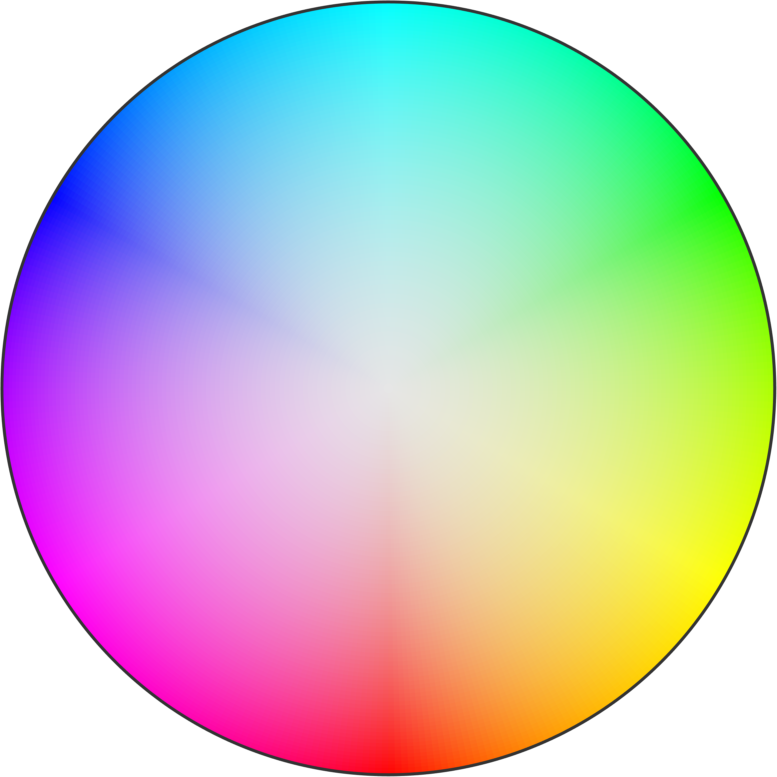
\includegraphics[width=0.155\textwidth]{ipfkeys/1}}
      &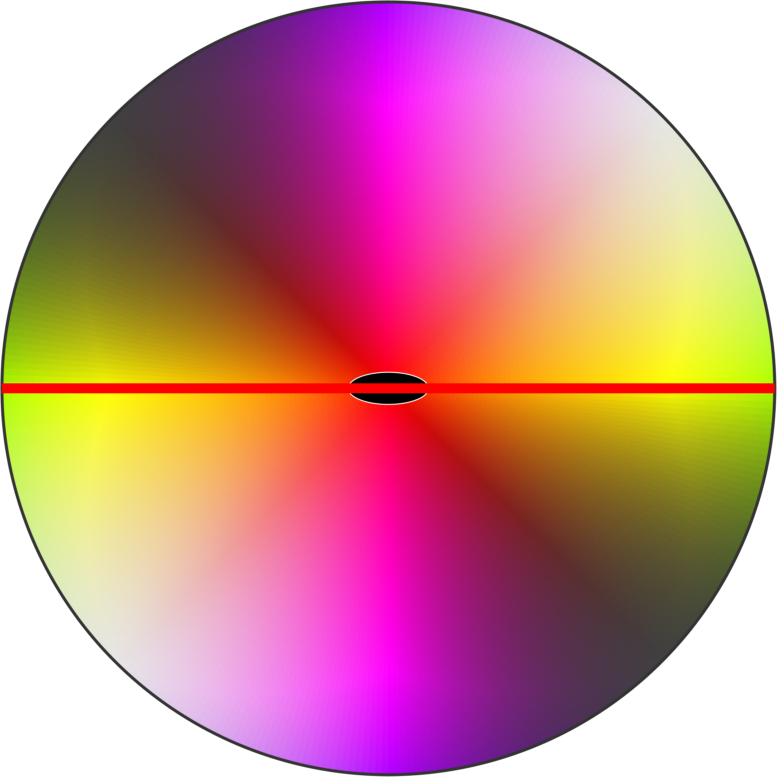
\includegraphics[width=0.155\textwidth]{ipfkeys/112}
      &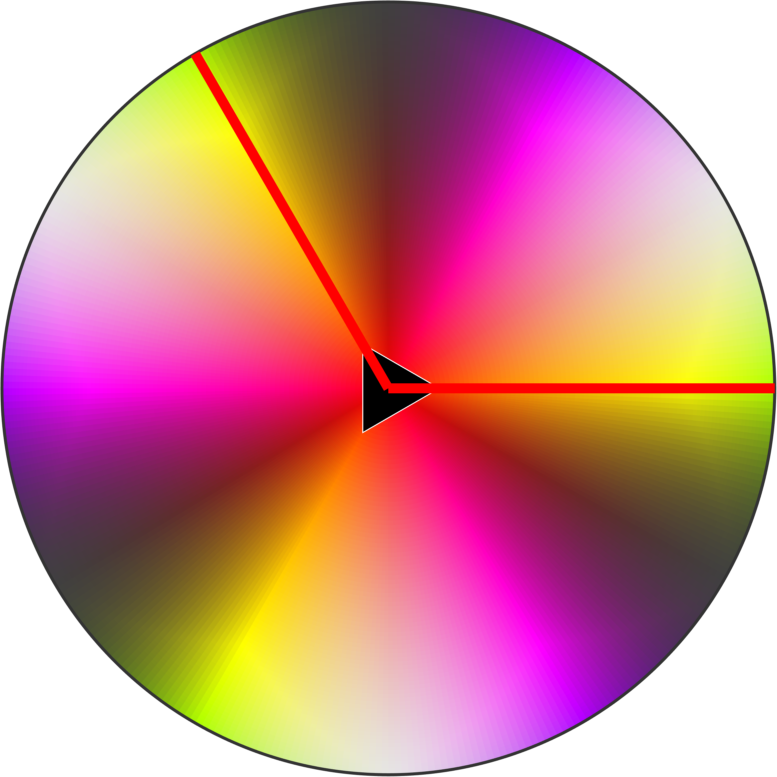
\includegraphics[width=0.155\textwidth]{ipfkeys/3}
      &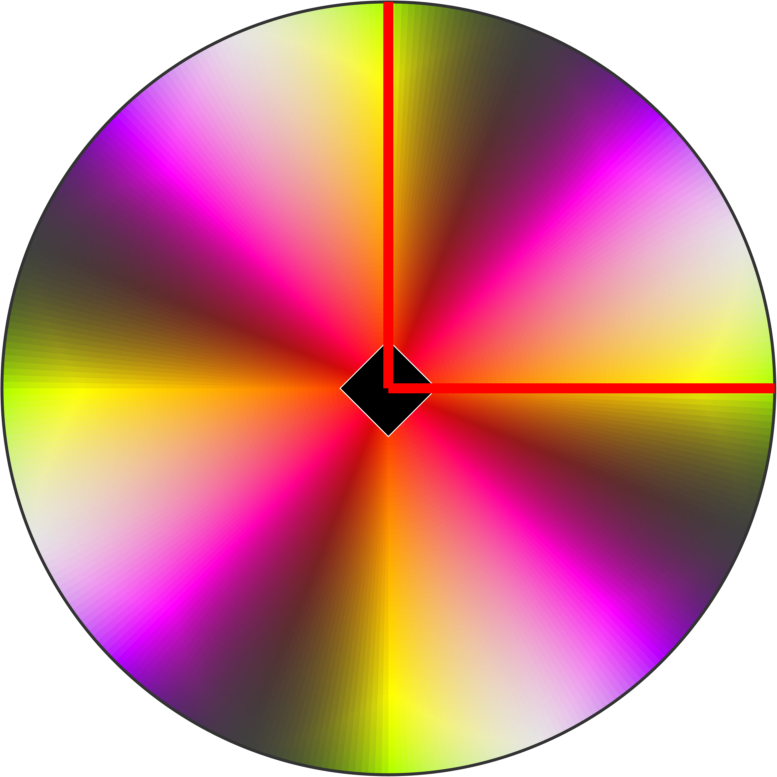
\includegraphics[width=0.155\textwidth]{ipfkeys/4}
      &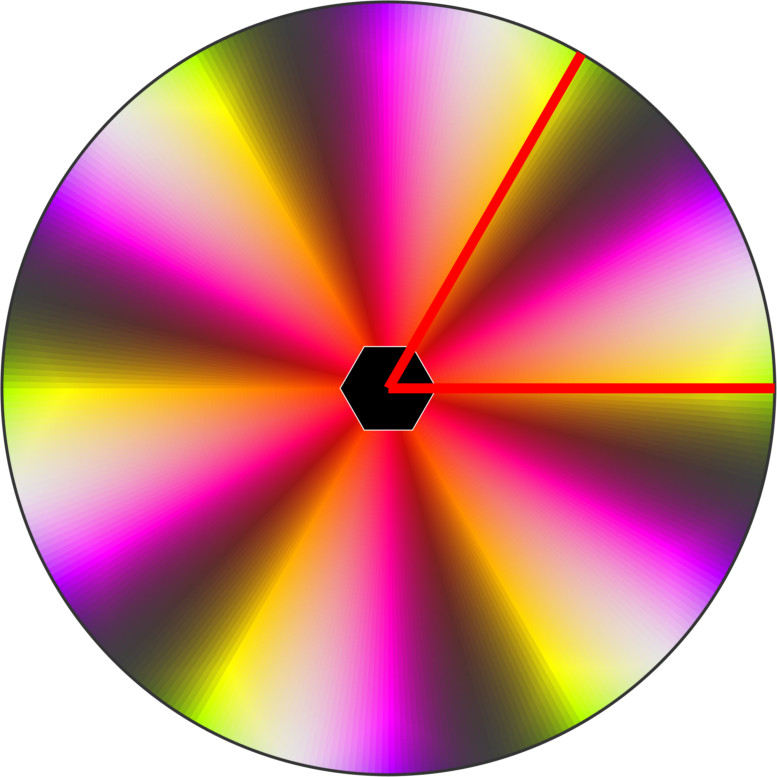
\includegraphics[width=0.155\textwidth]{ipfkeys/6}
      &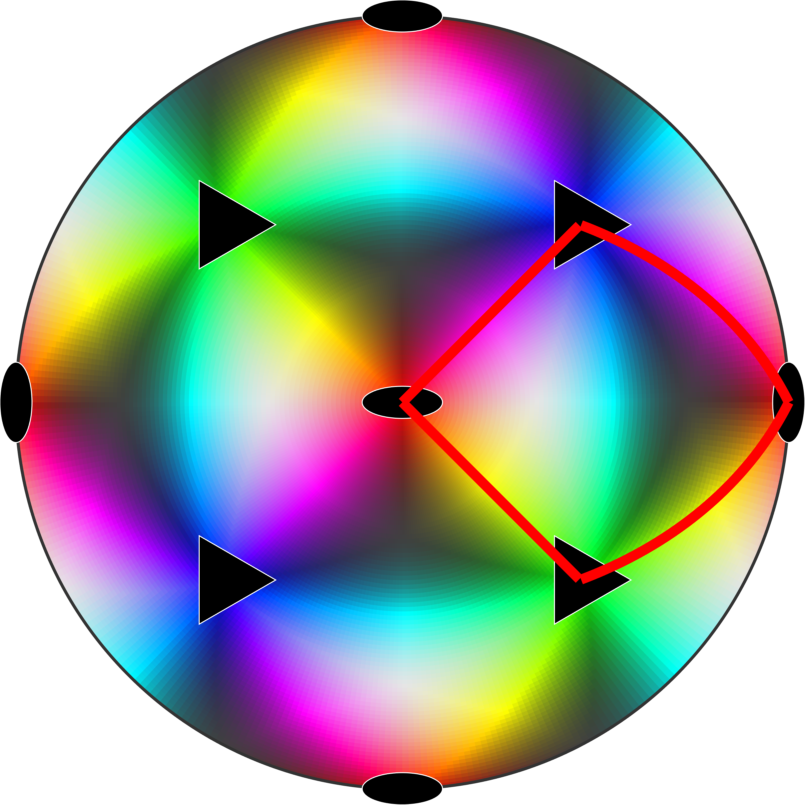
\includegraphics[width=0.155\textwidth]{ipfkeys/23}\\
      \multicolumn{1}{|c|}{1 $(\mathrm C_{1})$}
      & 2 $(\mathrm C_{2})$
      & 3 $(\mathrm C_{3})$
      & 4 $(\mathrm C_{4})$
      & 6 $(\mathrm C_{6})$
      & 23 $(\mathrm T)$ \\[1ex]
      \cline{1-2} %& 1 & 1 & & &\\
      &  orthorhombic & & & &\\
      &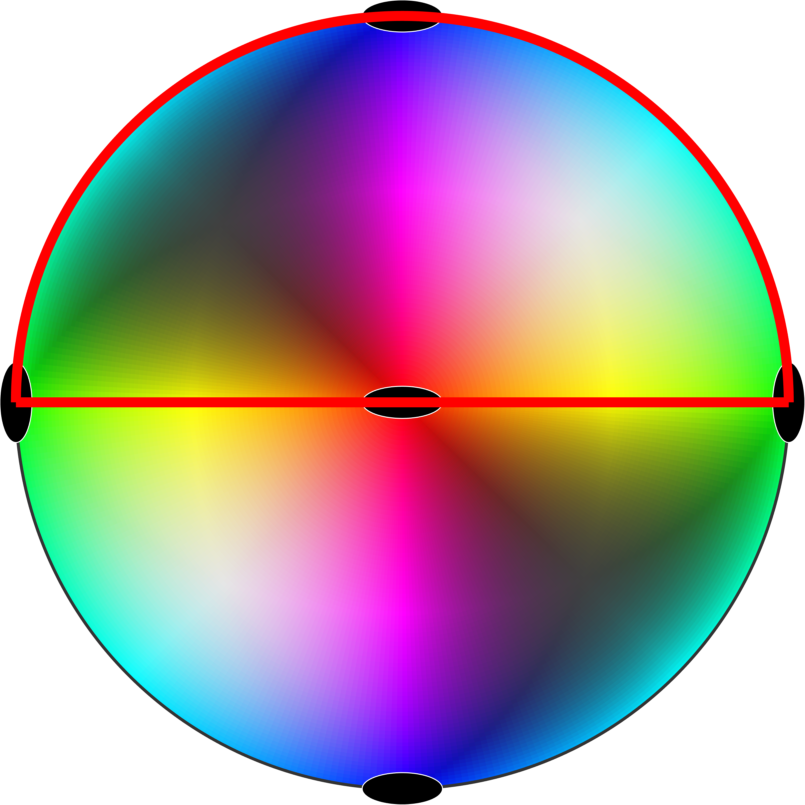
\includegraphics[width=0.155\textwidth]{ipfkeys/222}
      &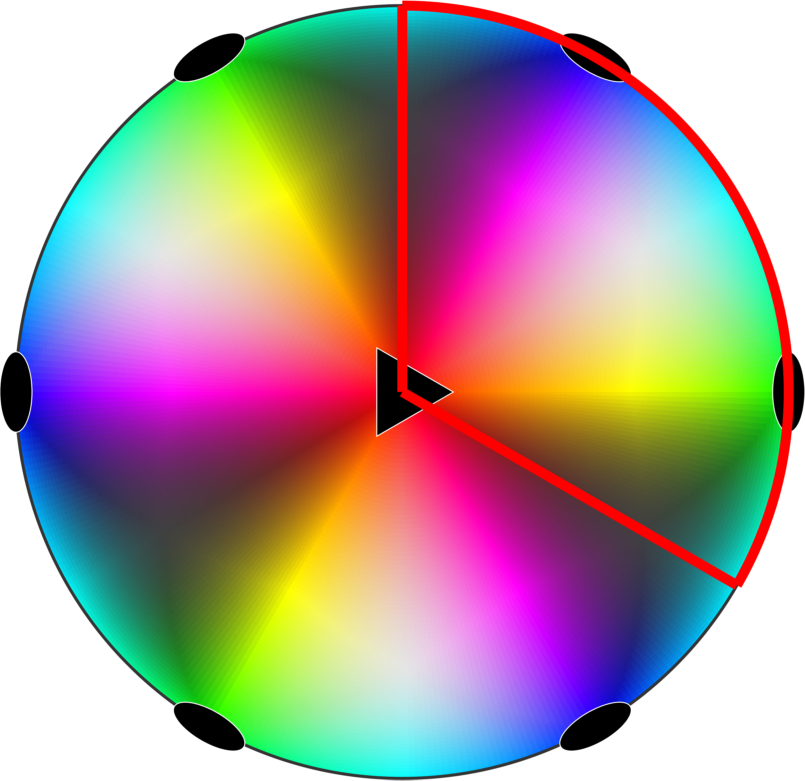
\includegraphics[width=0.155\textwidth]{ipfkeys/321}
      &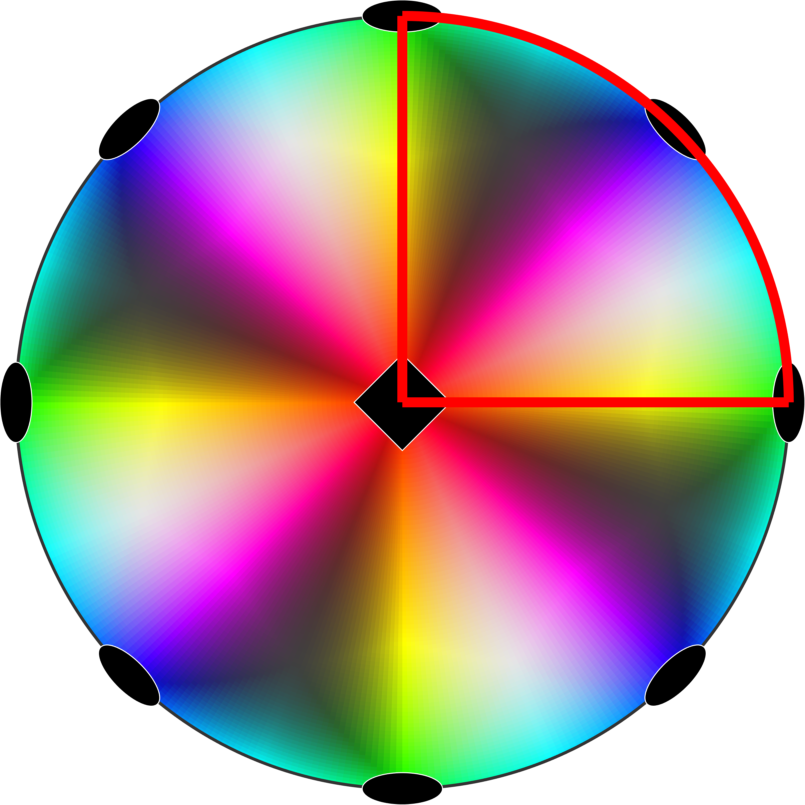
\includegraphics[width=0.155\textwidth]{ipfkeys/422}
      &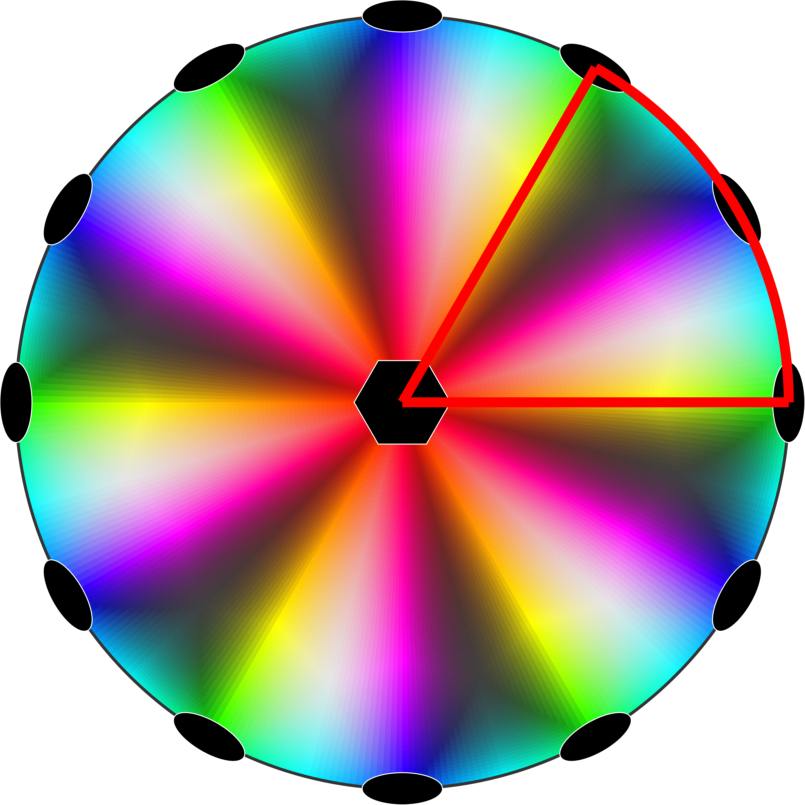
\includegraphics[width=0.155\textwidth]{ipfkeys/622}
      &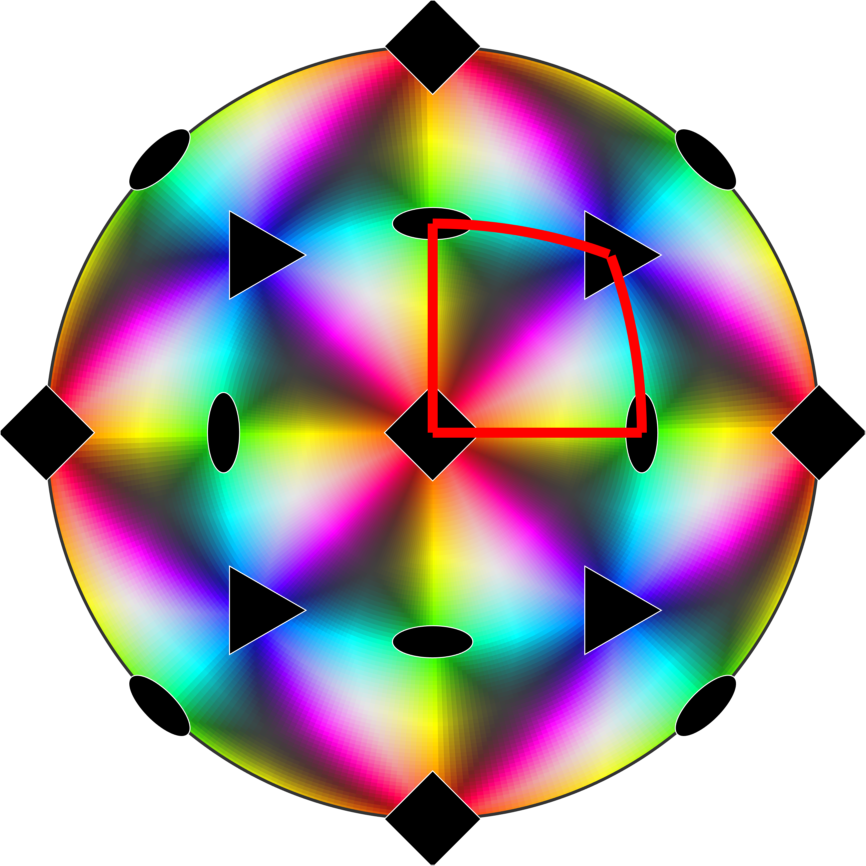
\includegraphics[width=0.155\textwidth]{ipfkeys/432}\\
      & 222 $(\mathrm D_{2})$
      & 321 $(\mathrm D_{3})$
      & 422 $(\mathrm D_{4})$
      & 622 $(\mathrm D_{6})$
      & 432 $(\mathrm O)$\\
      \cline{2-6}
    \end{tabular}
  \end{center}
\end{frame}


\begin{frame}
  \frametitle{IPF Color Keys for the Laue Groups}

  \begin{center}
    \setlength{\tabcolsep}{2pt}
    \begin{tabular}{c|c|c|c|c|c|}
      \hline
      \multicolumn{1}{|c|}{triclinic}
      & monoclinic
      & trigonal
      & tetragonal
      & hexagonal
      & cubic\\
      \multicolumn{1}{|c|}{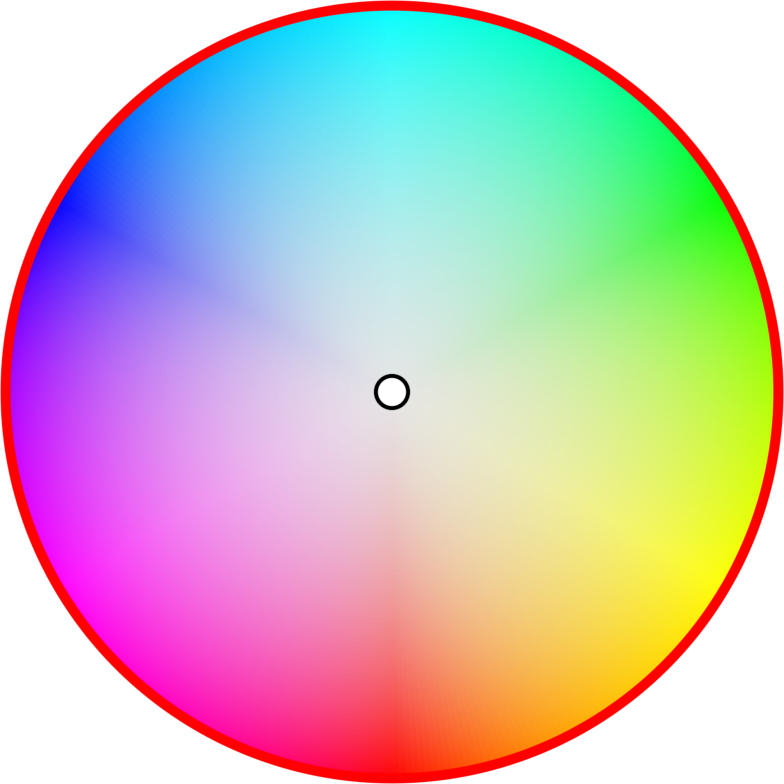
\includegraphics[width=0.155\textwidth]{ipfkeys/-1}}
      &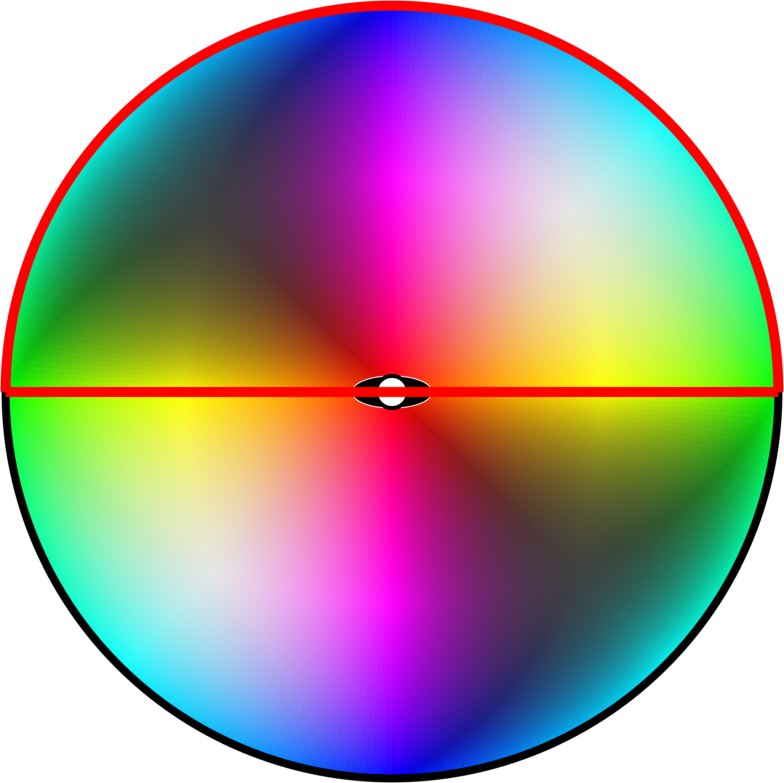
\includegraphics[width=0.155\textwidth]{ipfkeys/112_m}
      &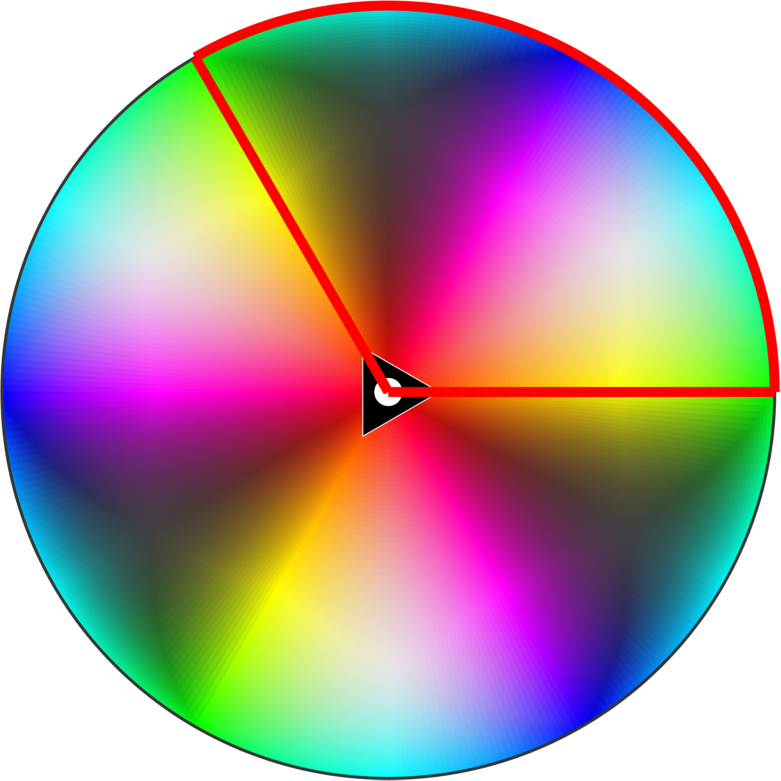
\includegraphics[width=0.155\textwidth]{ipfkeys/-3}
      &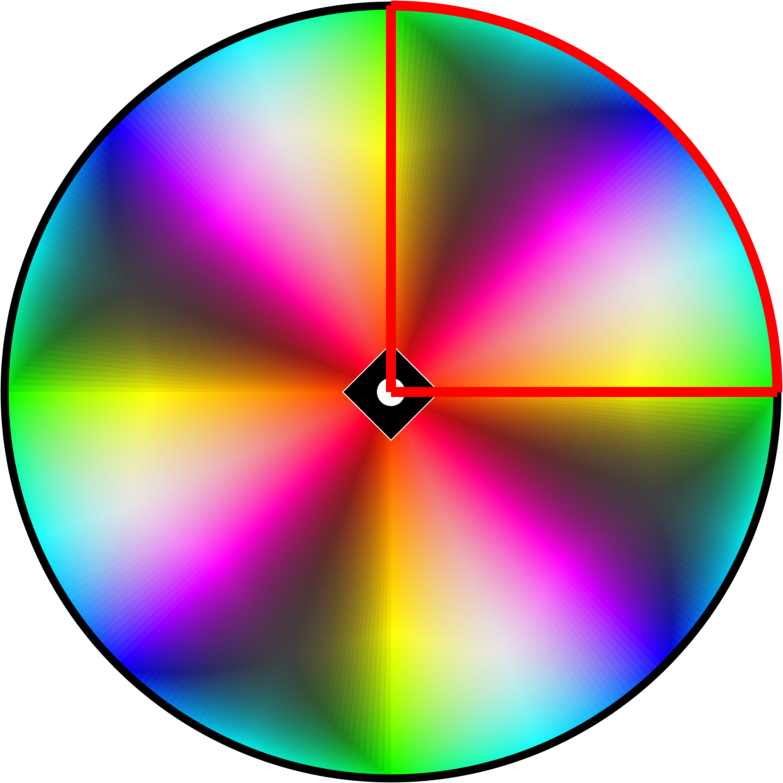
\includegraphics[width=0.155\textwidth]{ipfkeys/4_m}
      &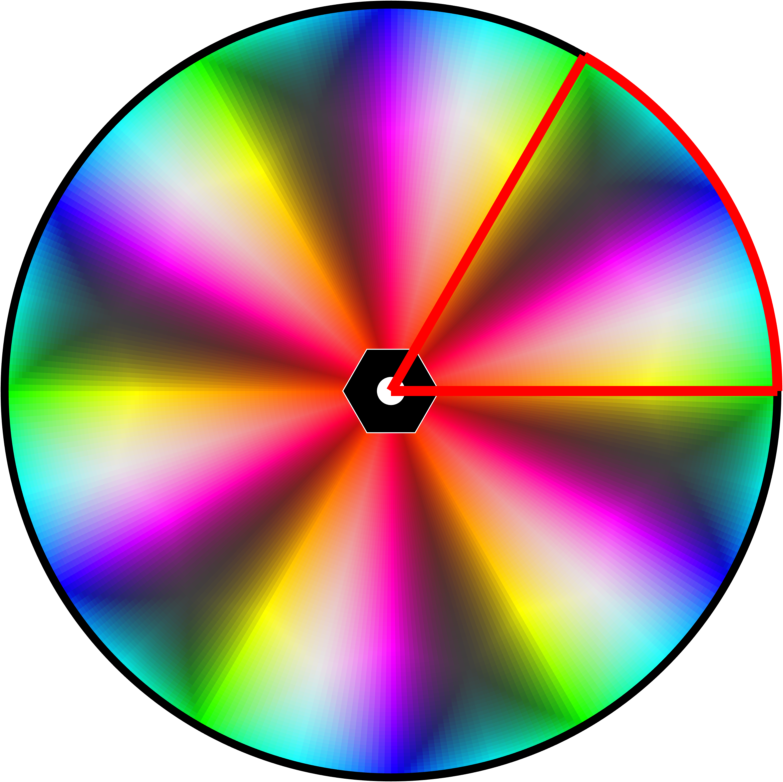
\includegraphics[width=0.155\textwidth]{ipfkeys/6_m}
      &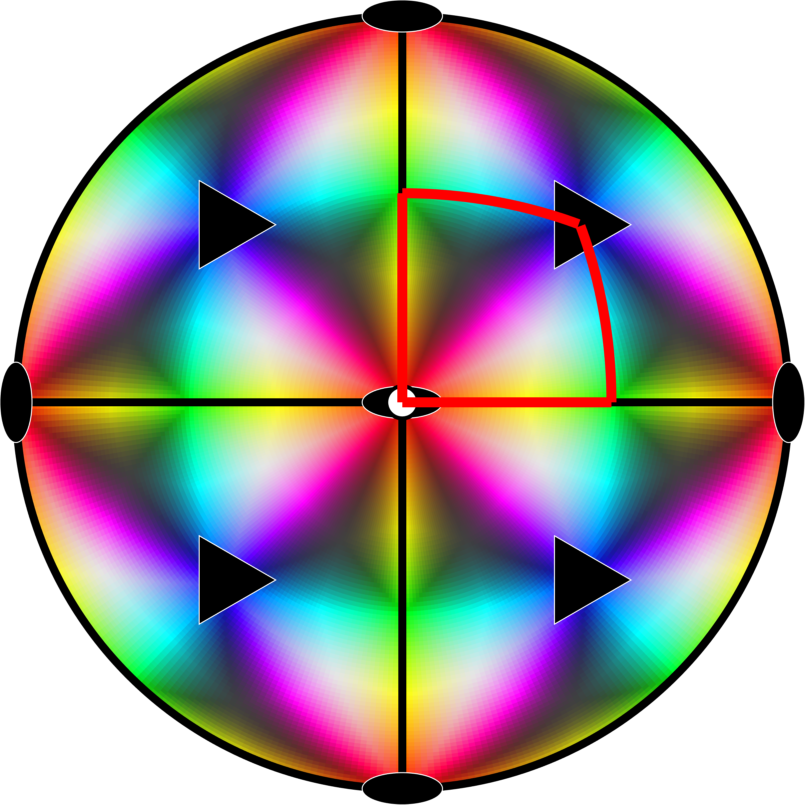
\includegraphics[width=0.155\textwidth]{ipfkeys/m-3}\\
      \multicolumn{1}{|c|}{\alert{$\overline{1}$ $(\mathrm C_{\mathrm i})$}}
      & $\frac{2}{\mathrm m}$ $(\mathrm C_{2\mathrm h})$
      & \alert{$\overline{3}$ $(\mathrm C_{3\mathrm i})$}
      & $\frac{4}{\mathrm m}$ $(\mathrm C_{4\mathrm h})$
      & $\frac{6}{\mathrm m}$ $(\mathrm C_{6\mathrm h})$
      & $\mathrm m\overline{3}$ $(\mathrm T_{\mathrm h})$ \\[1ex]
      \cline{1-2} %& 1 & 1 & & &\\
      &  orthorhombic & & & &\\
      &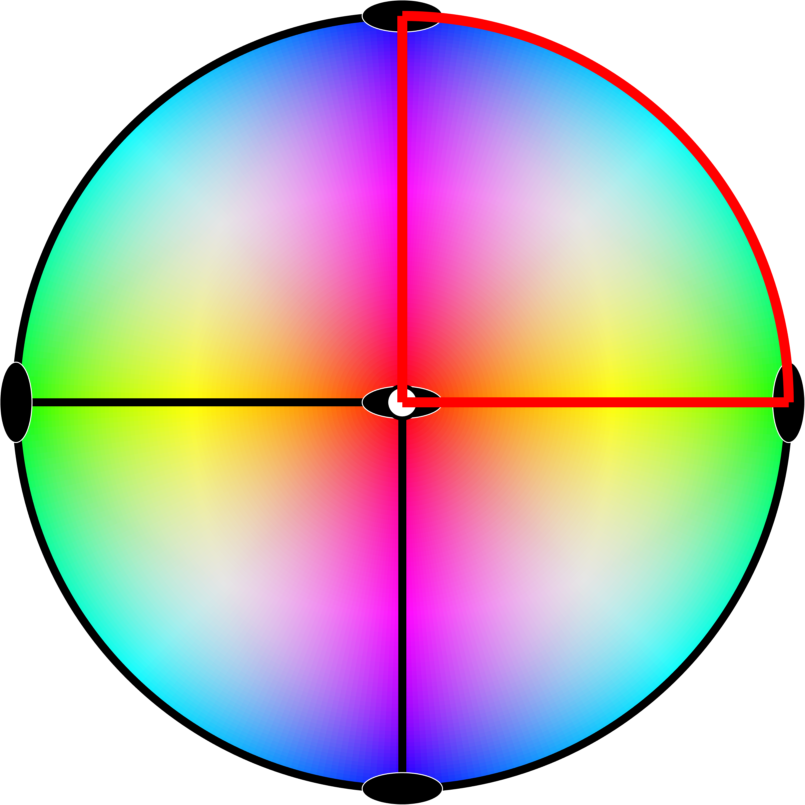
\includegraphics[width=0.155\textwidth]{ipfkeys/mmm}
      &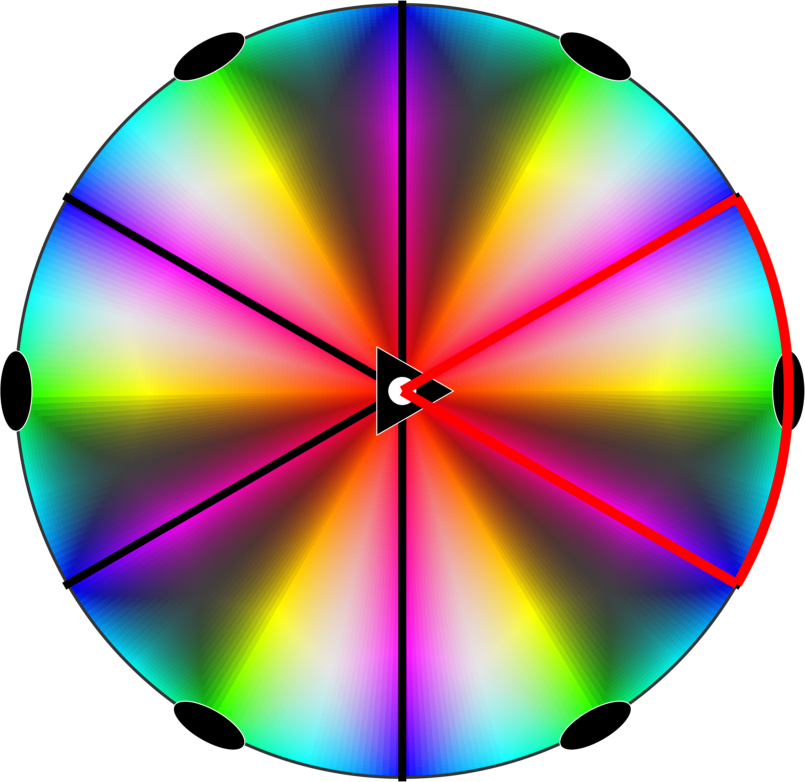
\includegraphics[width=0.155\textwidth]{ipfkeys/-3m1}
      &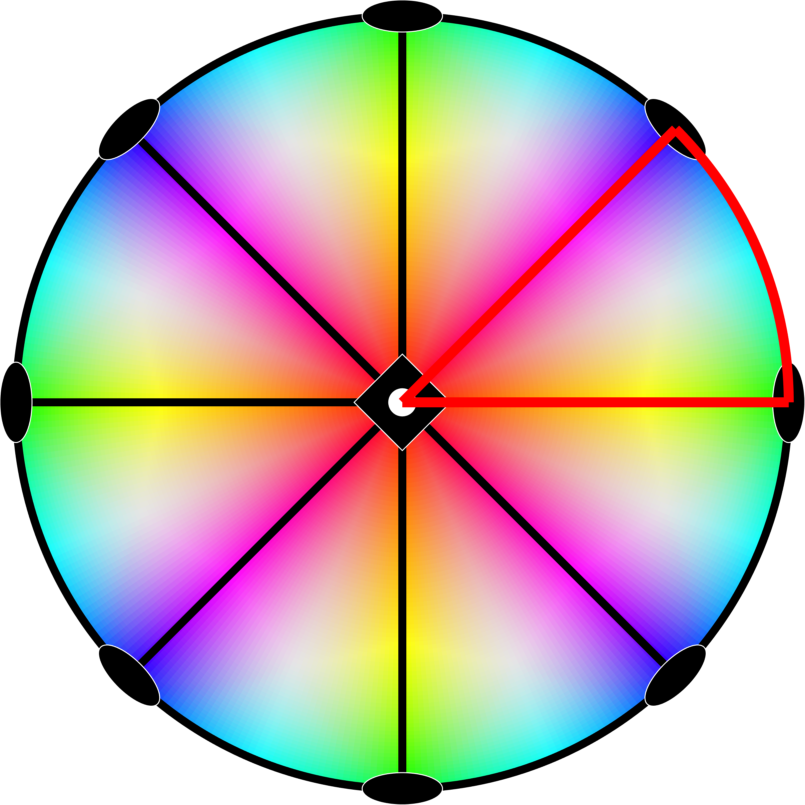
\includegraphics[width=0.155\textwidth]{ipfkeys/4_mmm}
      &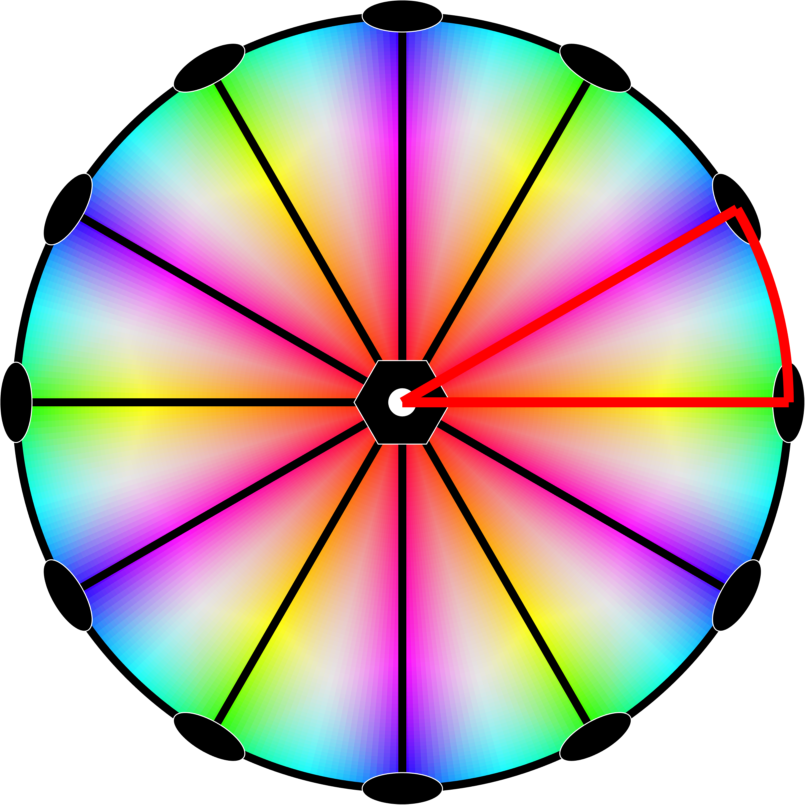
\includegraphics[width=0.155\textwidth]{ipfkeys/6_mmm}
      &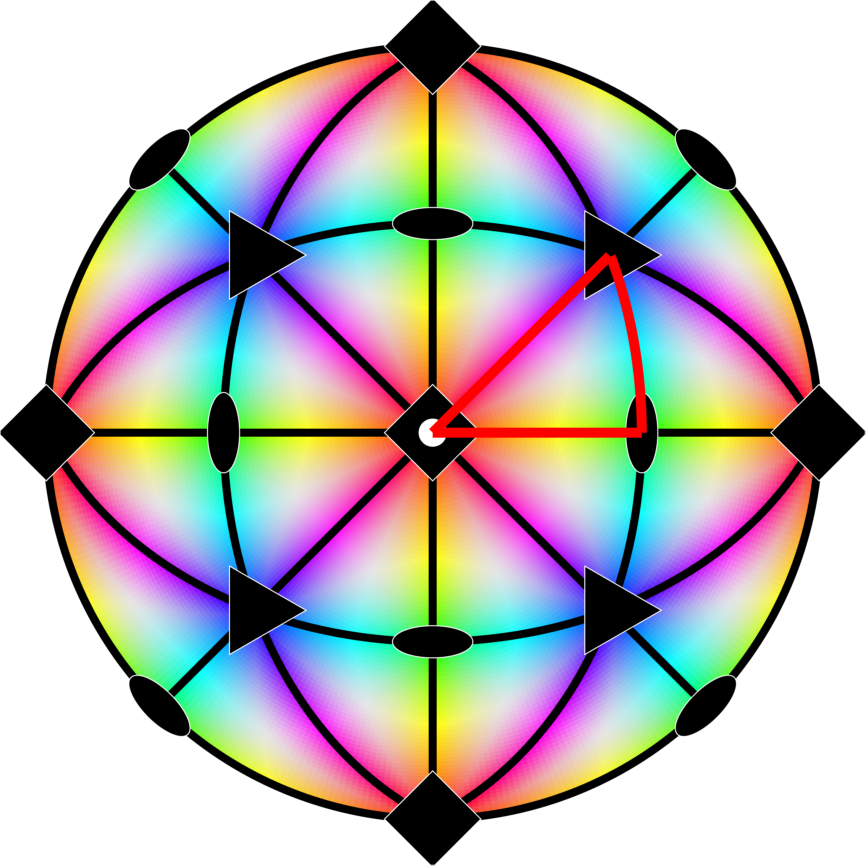
\includegraphics[width=0.155\textwidth]{ipfkeys/m-3m}\\
      & mmm $(\mathrm D_{2\mathrm h})$
      & $\overline{3}\mathrm m$ $(\mathrm D_{3\mathrm d})$
      & 4/mmm $(\mathrm D_{2\mathrm h})$
      & 6/mmm $(\mathrm D_{6\mathrm h})$
      & m$\overline{3}$m $(\mathrm O_{\mathrm h})$\\
      \cline{2-6}
    \end{tabular}
  \end{center}
\end{frame}


\begin{frame}
  \frametitle{IPF Color Keys for the Mixed groups}

\begin{center}
    \setlength{\tabcolsep}{2pt}
    \begin{tabular}{cccccc}
      \hline
      \multicolumn{1}{|c}{monoclinic}
      & \multicolumn{1}{|c}{orthorhombic}
      & \multicolumn{1}{|c}{trigonal}
      & \multicolumn{1}{|c}{tetragonal}
      & \multicolumn{1}{|c}{hexagonal}
      & \multicolumn{1}{|c|}{cubic}\\
      \multicolumn{1}{|c}{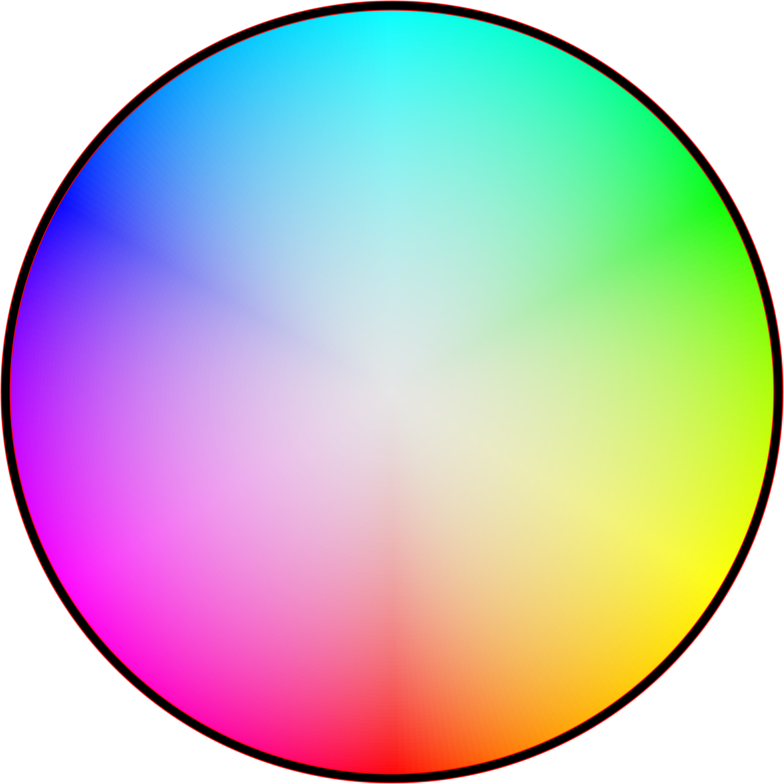
\includegraphics[width=0.155\textwidth]{ipfkeys/11m}}
      &\multicolumn{1}{|c}{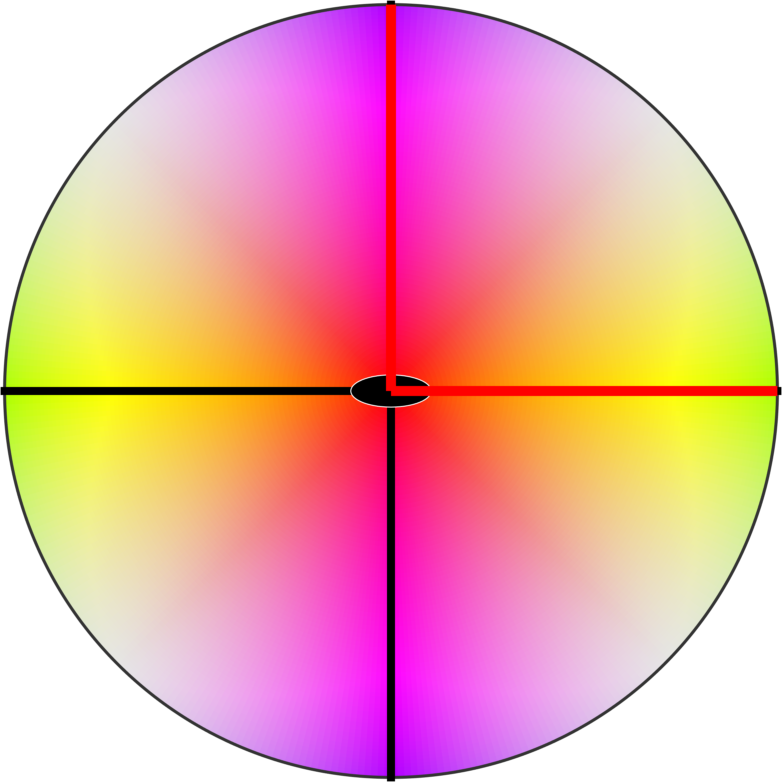
\includegraphics[width=0.155\textwidth]{ipfkeys/mm2}}
      &\multicolumn{1}{|c}{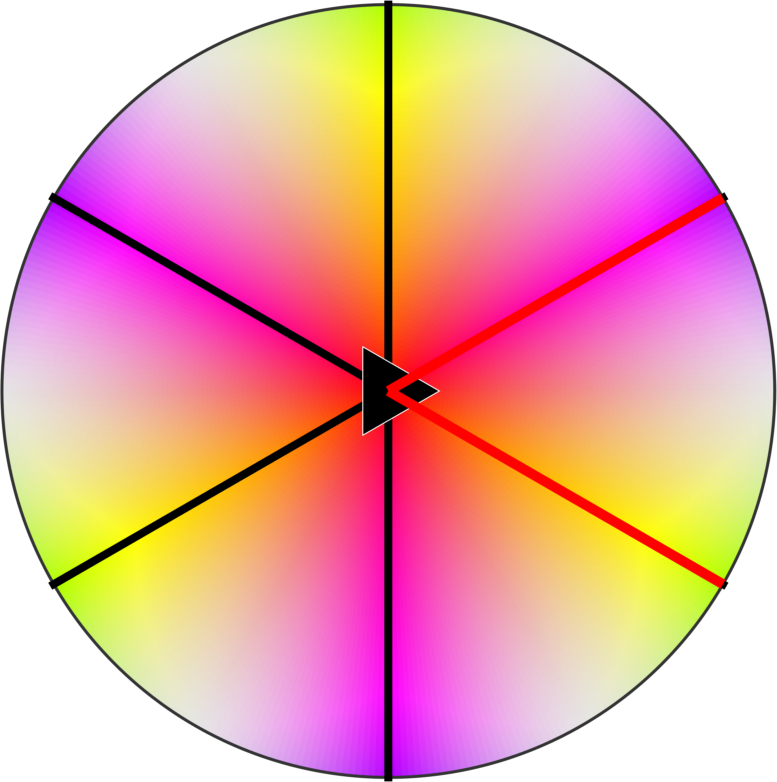
\includegraphics[width=0.155\textwidth]{ipfkeys/3m1}}
      &\multicolumn{1}{|c}{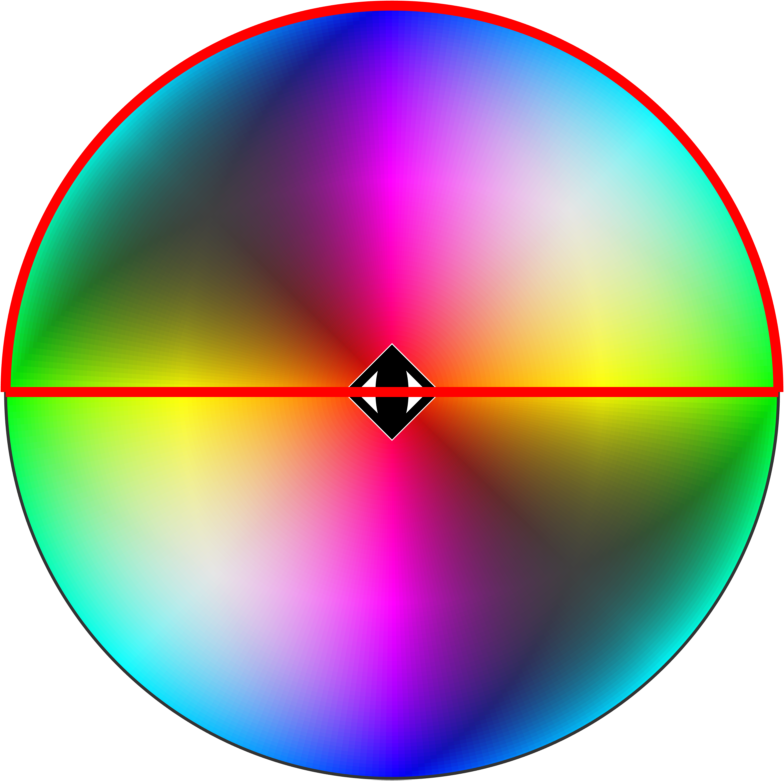
\includegraphics[width=0.155\textwidth]{ipfkeys/-4}}
      &\multicolumn{1}{|c}{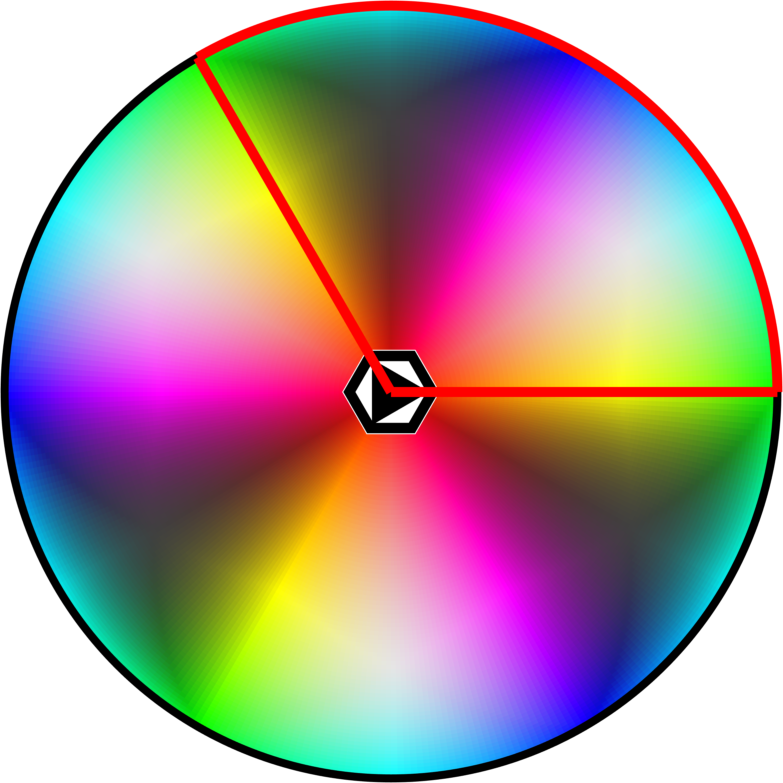
\includegraphics[width=0.155\textwidth]{ipfkeys/-6}}
      &\multicolumn{1}{|c|}{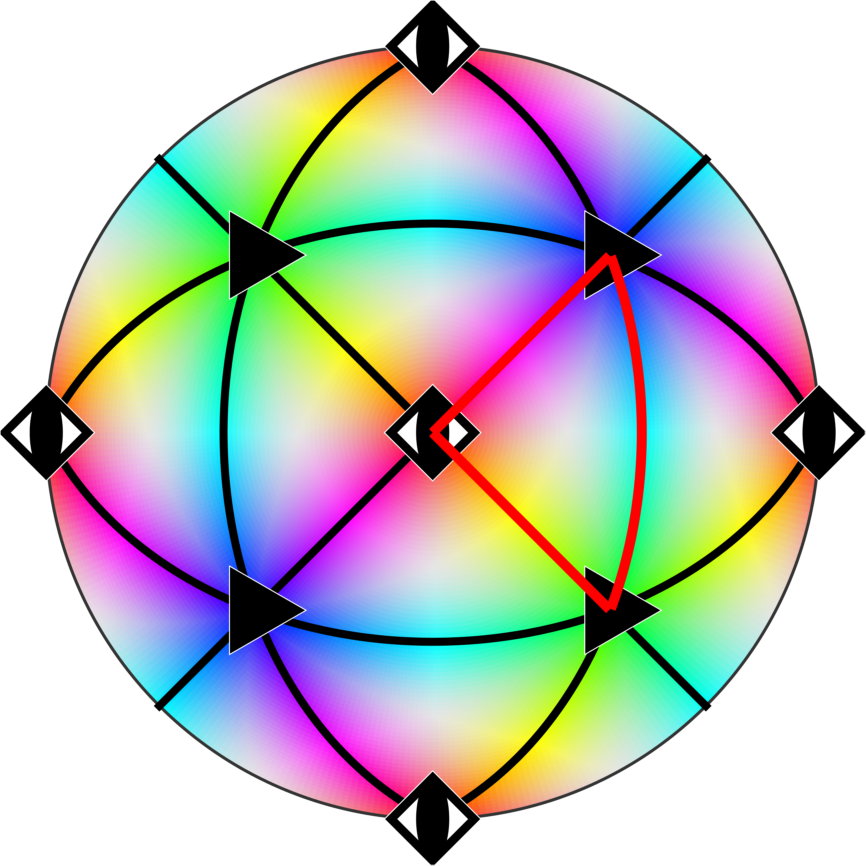
\includegraphics[width=0.155\textwidth]{ipfkeys/-43m}}\\
      \multicolumn{1}{|c}{$\overline{2}=\mathrm m$ $(\mathrm C_{\mathrm s})$}
      & \multicolumn{1}{|c}{$\mathrm m \mathrm m 2$ $(\mathrm C_{2\mathrm v})$}
      & \multicolumn{1}{|c}{$3 \mathrm m$ $(\mathrm C_{3\mathrm v})$}
      & \multicolumn{1}{|c}{\alert{$\overline{4}$ $(\mathrm S_{4})$}}
      &  \multicolumn{1}{|c}{$\overline{6}$ $(\mathrm C_{3\mathrm h})$}
      &  \multicolumn{1}{|c|}{
        $\overline{4}3\mathrm m$ $(\mathrm
        T_{\mathrm d})$} \\[1ex]
      \cline{1-3}\cline{6-6}
      & &
      \multicolumn{1}{|c}{} & & \multicolumn{1}{|c}{} & \multicolumn{1}{c|}{}\\
      &
      & \multicolumn{1}{|c}{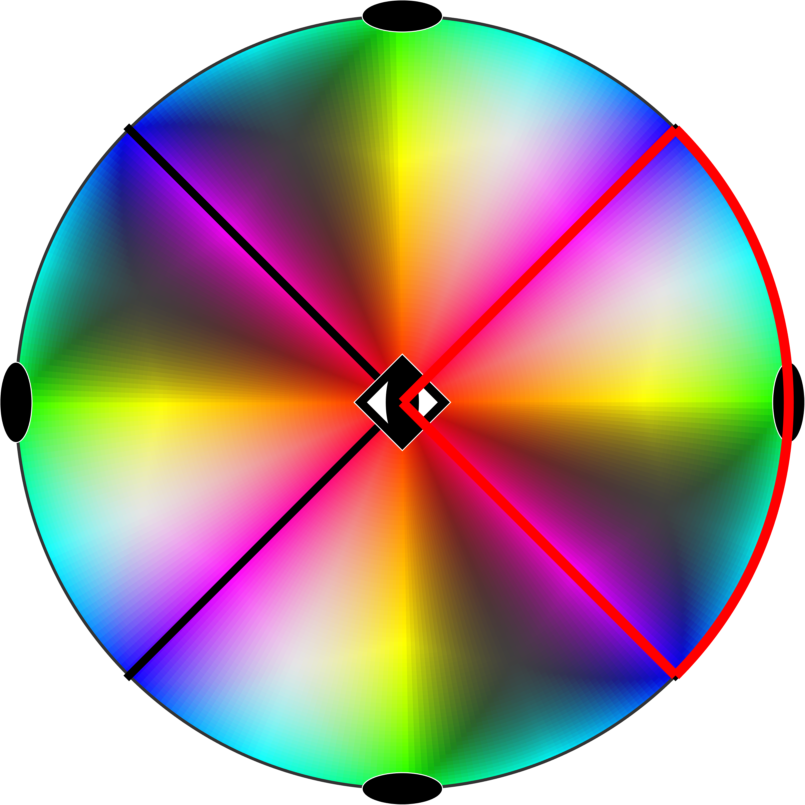
\includegraphics[width=0.155\textwidth]{ipfkeys/-42m}}
      & 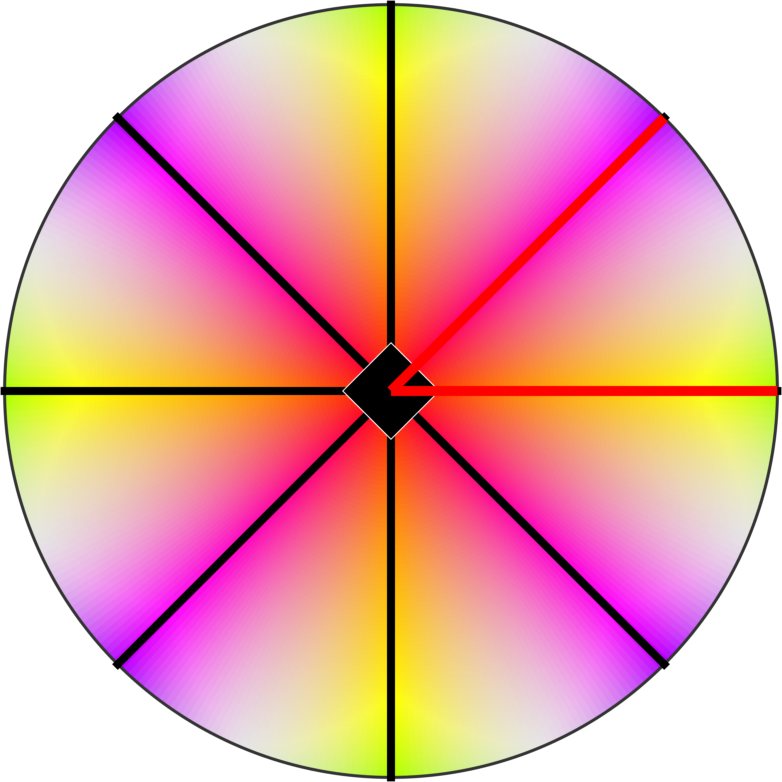
\includegraphics[width=0.155\textwidth]{ipfkeys/4mm}
      & \multicolumn{1}{|c}{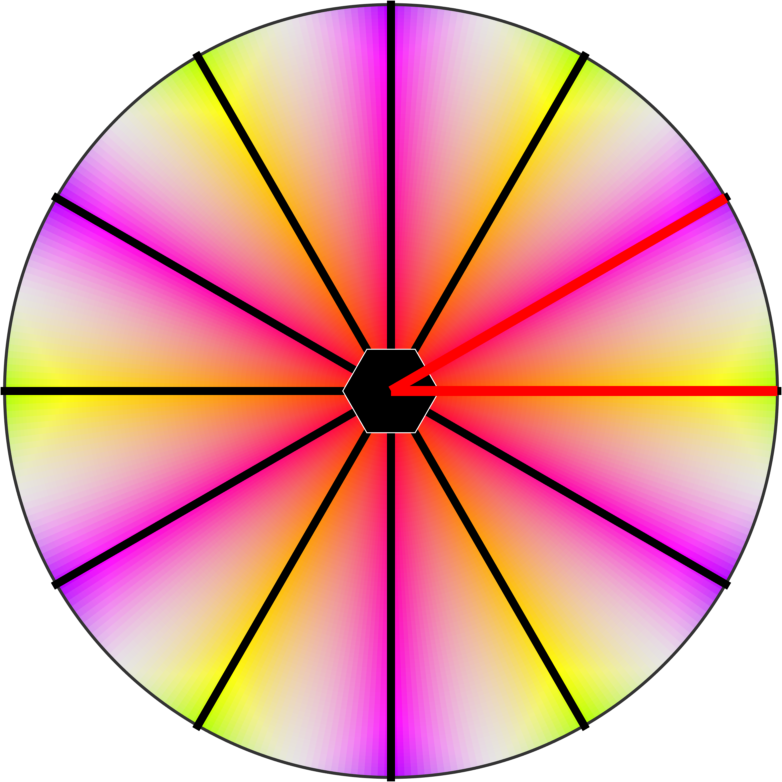
\includegraphics[width=0.155\textwidth]{ipfkeys/6mm}}
      & \multicolumn{1}{c|}{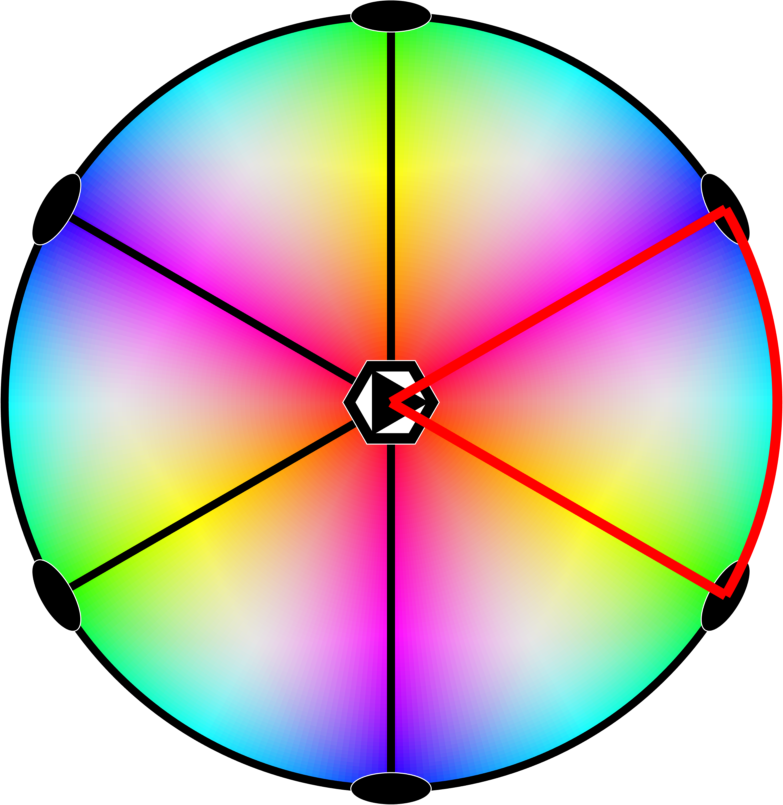
\includegraphics[width=0.155\textwidth]{ipfkeys/-6m2}}\\
      &
      & \multicolumn{1}{|c}{$\overline{4}2\mathrm m$ $(\mathrm D_{2\mathrm d})$}
      & 4mm $(\mathrm C_{4\mathrm v})$
      & \multicolumn{1}{|c}{6mm $(\mathrm C_{6\mathrm v})$}
      & \multicolumn{1}{c|}{$\overline{6}$m2 $(\mathrm D_{3\mathrm h})$}\\
      \cline{3-6}
    \end{tabular}
  \end{center}

\end{frame}




\end{document}
